%\documentclass[10pt,final]{flbook12}
%\documentclass[10pt,draft]{flwide10}
\documentclass[10pt,final]{flwide10}


  %\usepackage[LY1]{fontenc}
  %\usepackage[LY1,mtbold]{pupfonts}
  \usepackage[LY1,mtbold]{}
  \usepackage{bm}
  \usepackage{epsfig}
  \usepackage{latexsym}
  \usepackage{makeidx}
  % Our own definitions
  \RequirePackage{subfigure}
\RequirePackage{graphicx}
\RequirePackage{color,graphics}
\RequirePackage{caption}
\RequirePackage{amsmath} % This is for numbering equations
\RequirePackage{listings}


% The scale for figures

\newcommand{\scale}{0.3}
\newcommand{\linescale}{0.6}
\newcommand{\smallscale}{0.5}

\captionsetup{margin=10pt,font=small,labelfont=bf}

% ------------------- Other definitions

\newcommand{\ejs}{\emph{EjsS}}
\newcommand{\Ejs}{\emph{Easy Java/JavaScript Simulations}}
\newcommand{\osp}{\emph{OSP}}
\newcommand{\Osp}{\emph{Open Source Physics}}

\newcommand{\file}[1]{\textbf{#1}} % the name of a file or directory
\newcommand{\code}[1]{{\ttfamily #1}} % a variable

\newcommand{\url}[1]{{\ttfamily #1}} % a variable
\newcommand{\lit}[1]{{\sl #1}}  % literal text
%\newcommand{\lit}[1]{``#1''}  % literal text
\newcommand{\link}[1]{\emph{$<$#1$>$}}  %URL Links
\newcommand{\note}[1]{\begin{quote}\small #1\end{quote}}  % a big note with color background

%Use special environments for listings, exercises, problems, and projects.
\newenvironment{listing} {\ttfamily\small}{}
%exerciseEnv is used to define the exercise environment
\newtheorem{exerciseEnv}{\hspace{-\parindent} Exercise}[chapter]
%The exercise environment adds a box at the end of the exercise narrative to indicate the end of the exercise.
\newenvironment{exercise}[1][]{\begin{exerciseEnv}{\textbf{#1}\newline}}{\boldmath $\Box$ \end{exerciseEnv}}
%problems and projects appear at the end of each chapter
\newtheorem{problem}{\hspace{-\parindent} Problem}[chapter]
\newtheorem{project}{\hspace{-\parindent} Project}[chapter]

% environments for long listings
\definecolor{background}{rgb}{1,1,1}
\definecolor{sepcolor}{rgb}{0.90,0.90,0.90}
\lstset{language=Java,
linewidth=30pc,
showstringspaces=false,
commentstyle=\upshape,
stringstyle=\ttfamily,
%basicstyle=\small,
basicstyle=\scriptsize\ttfamily\baselineskip10pt, breaklines=true, keywordstyle=\upshape,
breakatwhitespace=true, morecomment=[is]{/*}{*/}, moredelim=**[is][\hfill\bfseries]{/*+}{+*/},
moredelim=[is][\emph]{+-}{-+}, moredelim=[is][\emph]{/*-}{-*/}} 

  \makeindex

  %\includeonly{01Introduction/mainIntro,02ExplorationJava/mainJava}
  %\includeonly{01Introduction/mainIntro,03ExplorationJavascript/mainJS}
 % \includeonly{04JavatoJS/mainJavaToJS}
 % \includeonly{appendixA/mainEvents}

\begin{document}

  \frontmatter
  \title{\Ejs\ Manual}

    %\shorttitle{Modeling Science}
    %\subtitle{None}

  \author{\center Wolfgang Christian \linebreak and \linebreak Francisco Esquembre}

    %\makehalftitle
    \maketitle

% ------------------------------------------
  \frontmatter
    %\include{preface/foreword}
    %\tableofcontents

% ------------------------------------------
  \mainmatter
 
      % !TEX root = ../Guide de l'utilisateur de EjsS.tex

\chapter{Installation et ex�cution de \Ejs}\label{chapter:EjsIntro}

\begin{quote}
Les machines doivent travailler. Les personnes penser.  {\em Richard Hamming}
\end{quote}

Ce chapitre d'introduction nous offre une vue d'ensemble sur \Ejs\ -- Simulations Simples en Java/JavaScript -- (\ejs\ sous forme abr�g�e),  l'outil de mod�lisation et de cr�ation de haut niveau que nous utilisons pour enseigner la mod�lisation et la simulation. Nous allons premi�rement d�crire le processus d'installation et la structure de fichiers de notre programme et par la suite ex�cuter la console \ejs\  pour obtenir notre premier programme \ejs\  sur l'�cran. Nous d�crivons comment \Ejs\  supporte des diff�rents langages de programmation pour le processus de mod�lisation. Les chapitres ult�rieurs de ce document fournissent une introduction �tape par �tape des diff�rentes parties de l'interface graphique utilisateur. Finalement nous vous donnons les instructions pour t�l�charger les mod�les cr��s avec \ejs\ existants sur notre biblioth�ques num�riques en ligne.

% ------------------------
  \section{� propos d' \Ejs}
% ------------------------

La mod�lisation informatique est intimement li�e � la simulation informatique. Un mod�le est une repr�sentation conceptuelle d'un syst�me physique et de ses propri�t�s, la mod�lisation est le processus par lequel nous �laborons cette repr�sentation. La mod�lisation informatique n�cessite de (1) la description et de l'analyse d'un probl�me, (2) de l'identification des variables et des algorithmes, (3) de la mise en oeuvre sur une plate-forme de mat�riel et logiciel, (4) de l'ex�cution de l'impl�mentation et de l'analyse des r�sultats, (5) de l'affinage et de la g�n�ralisation et (6) de la pr�sentation des r�sultats. Une simulation informatique est une impl�mentation qui nous permet de tester le mod�le sous de diff�rentes conditions dans le but d'apprendre sur le comportement du mod�le. L'applicabilit� des r�sultats de la simulation � ceux du syst�me (physique) authentique d�pend de jusqu'� quel point le mod�le d�crit la r�alit�. La science consiste � mettre au point des mod�les plus g�n�raux ou plus pr�cis.  

 L'impl�mentation d'un mod�le et la visualisation des donn�es de sortie nous force � programmer un ordinateur. Programmer peut �tre amusant parce que cela nous donne un contr�le total de tous les d�tails visuels et num�riques du monde simul�. Mais programmer c'est aussi une t�che technique qui peut intimider. Cependant cette barri�re technique peut �tre r�duite  si vous utilisez un outil appropri�. \Ejs\  est un outil de mod�lisation qui a �t� con�u pour permettre aux scientifiques, et non seulement aux scientifiques d'informatique, de cr�er des simulations dans de diff�rents langages de programmation.~\footnote{Actuellement, \ejs\ supporte les langages de programmation Java et Javascript.}  \ejs\  simplifie cette t�che autant d'un point de vue technique comme conceptuel.  

 \ejs\  nous fournit une simple mais puissante structure conceptuelle pour �laborer des simulations. Cet outil fournit une s�quence de panneaux de travail pour impl�menter le mod�le et l'interface graphique utilisateur. \ejs\ automatise des t�ches telles que la r�solution num�rique d'�quations diff�rentielles ordinaires et l'animation (en utilisant des traits s�par�s, en cas n�cessaire). La  communication de bas niveau entre le programme et l'utilisateur final qui a lieu lors de l'ex�cution, qui inclut le traitement des actions de la souris dans l'interface graphique de simulation, s'accomplit sans une  programmation de bas niveau.

 �videmment une partie du travail d�pend toujours de nous. Vous devez fournir un mod�le pour le ph�nom�ne et concevoir et s�lectionner une visualisation des donn�es de sortie qui montre les principales caract�ristiques du mod�le. Ces t�ches de haut niveau sont plus li�es � la science qu'� la programmation. Nous vous encourageons de consacrer votre temps et �nergie � �tudier la science, t�che que l'ordinateur ne peut pas faire. L'objet de ce document est de prouver que cette mod�lisation par ordinateur n'est non seulement possible pour les non-programmeurs, mais aussi relativement facile, � l'aide de \Ejs.
 
% ------------------------
    \section{Installer et executer le logiciel}\label{section:02Installation}\index{\Ejs!installing and running}
% ------------------------

Commen�ons par installer  et ex�cuter \Ejs. \ejs\  est un programme Java qui peut s'ex�cuter sous tout syst�me d'exploitation qui supporte une Machine Virtuelle (VM en anglais) Java. Comme Java est con�ue comme une plate-forme ind�pendante, l'interface utilisateur \ejs\  sur Mac OS X, Windows et Linux pr�sente une apparence tr�s similaire bien qu'il puisse y avoir quelques petites diff�rences. (Nous montrons l'interface Mac OS X dans les illustrations de ce document.) 

Si  \Ejs\ n'est pas install� sur votre ordinateur, vous devez l'installer. Pour \textbf{installer} \ejs, suivez ces indications:

\begin{numberlist}

\item \textbf{Installez Java Runtime Environment.} \ejs\ n�cessite de Java Runtime Environment (JRE)  --- l'environnement d'exploitation de Java --- \textbf{version 1.8 ou ult�rieure}.  C'est possible que le JRE soit d�j� install� sur votre ordinateur mais s'il ne l'est pas, visitez le site Java sur \link{http://java.com} et suivez les instructions pour t�l�charger et installer la derni�re version. 

\item \textbf{Copiez le fichier d'installation de \ejs\ sur votre ordinateur.} \ejs\ est distribu� dans un dossier compress� ZIP qui peut �tre t�l�charg� sur le site web de \ejs\  \link{http://www.um.es/fem/EjsWiki}. Le fichier d'installation sera intitul� d'une mani�re similaire � celui-ci: \file{EjsS\_X.x\_yymmdd.zip}. Les caract�res  \file{X.x} indiquen la version actuelle du logiciel et  \file{yymmdd} indique la date � laquelle cette version a �t� cr��e. (Par exemple vous pouvez obtenir un titre similaire � \file{EjsS\_5.2\_161123.zip}.)

\item \textbf{D�compressez  \ejs.} D�compressez le fichier d'installation \ejs\ sur le disque dur de votre ordinateur pour cr�er un r�pertoire intitul�  \file{EjsS\_X.x} (\file{EjsS\_5.2} dans l'exemple). Le nouveau r�pertoire contient le programme \ejs\ complet.

\note{Dans les syst�mes comme Unix, le r�pertoire \file{EjsS\_X.x} peut-�tre d�compress� comme � lecture seule. Activez les acc�s d'�criture pour le r�pertoire \file{EjsS\_X.x}  et tous ses sous-r�pertoires.}

\end{numberlist}

Et voil�!  C'est tout ce que vous devez faire pour installer \ejs. Une fois que  \Ejs\  est install� sur votre ordinateur, suivez ces indications pour \textbf{ex�cuter} \ejs:

\begin{description}
\item \textbf{Ex�cutez la console \ejs.} Dans le r�pertoire \file{EjsS\_X.x} r�cemment cr��, vous trouverez un fichier intitul� \file{EjsConsole.jar}.\index{jar files!EjsConsole.jar}\index{Easy Java Simulations!console} Double-cliquez pour ex�cuter la console \ejs\ comme indiqu� dans la figure~\ref{fig:01Introduction/EjsConsole}.

\note{ Si le double-clic n'ex�cute pas la console, ouvrez une fen�tre de terminal, changez au r�pertoire \file{EjsS\_X.x} et tapez la commande: \code{java-jar EjsConsole.jar}. Vous devrez �crire le nom complet de la commande Java s'il n'est pas dans le \lit{PATH} de votre syst�me.}
\end{description}


\begin{figure}[htb]
  \centering
%  \subfigure[Console's basic options tab.]{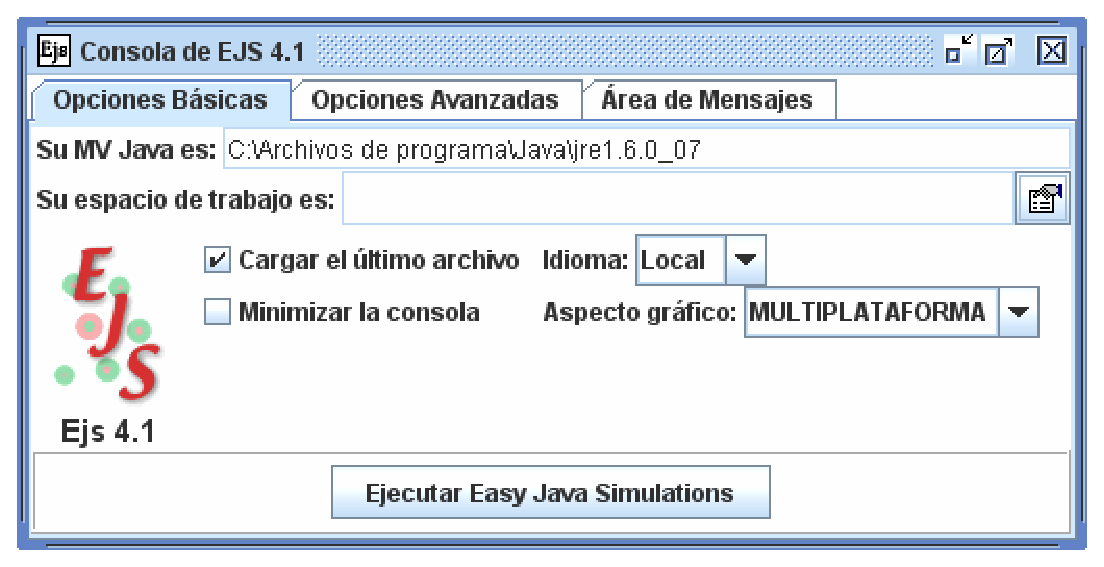
\includegraphics[scale=\scale]{01Introduction/images/EjsConsole1.eps}}
%  \subfigure[Console's output area.]{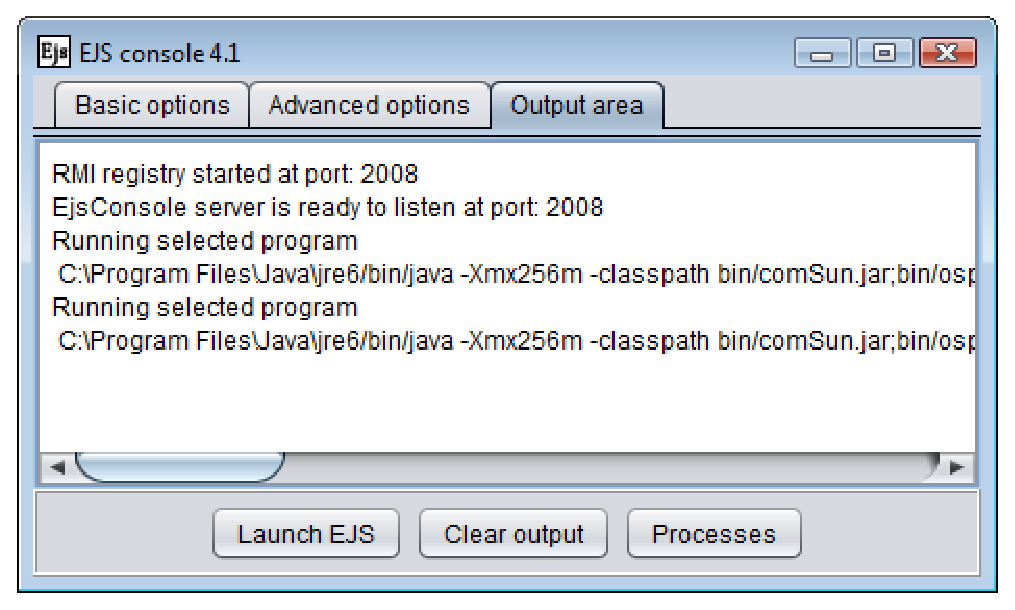
\includegraphics[scale=\scale]{01Introduction/images/EjsConsole2.eps}}
%  \caption{Two views of the \ejs\ console.}
  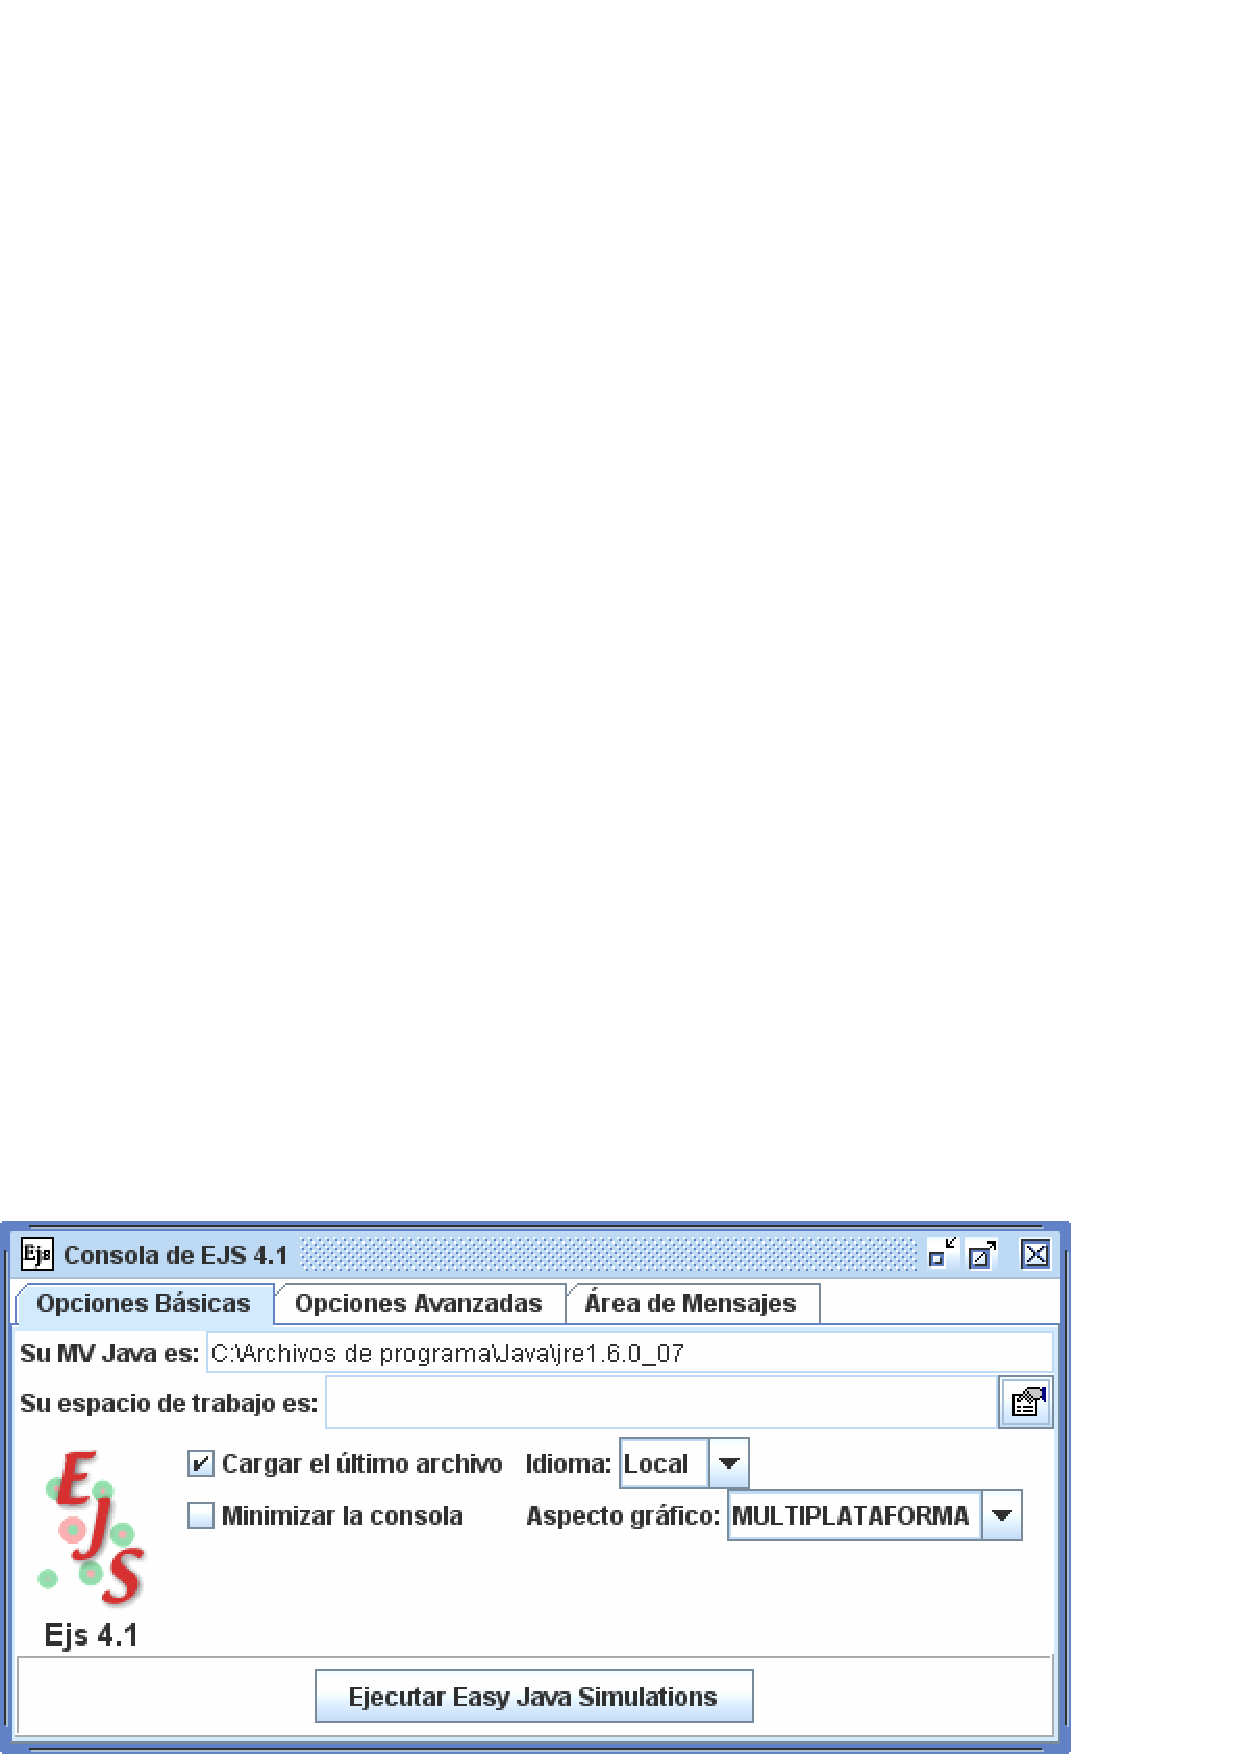
\includegraphics[scale=\scale]{01Introduction/images/EjsConsole1.png}
  \caption{La console \ejs.}
  \label{fig:01Introduction/EjsConsole}
\end{figure}

Vous devriez voir la console (Figure~\ref{fig:01Introduction/EjsConsole}) et le dialogue de s�lection de fichiers de la figure~\ref{fig:01Introduction/WorkspaceChooser}, d�crite ci-dessous, sur votre �cran.


\begin{figure}[htb]
  \centering
  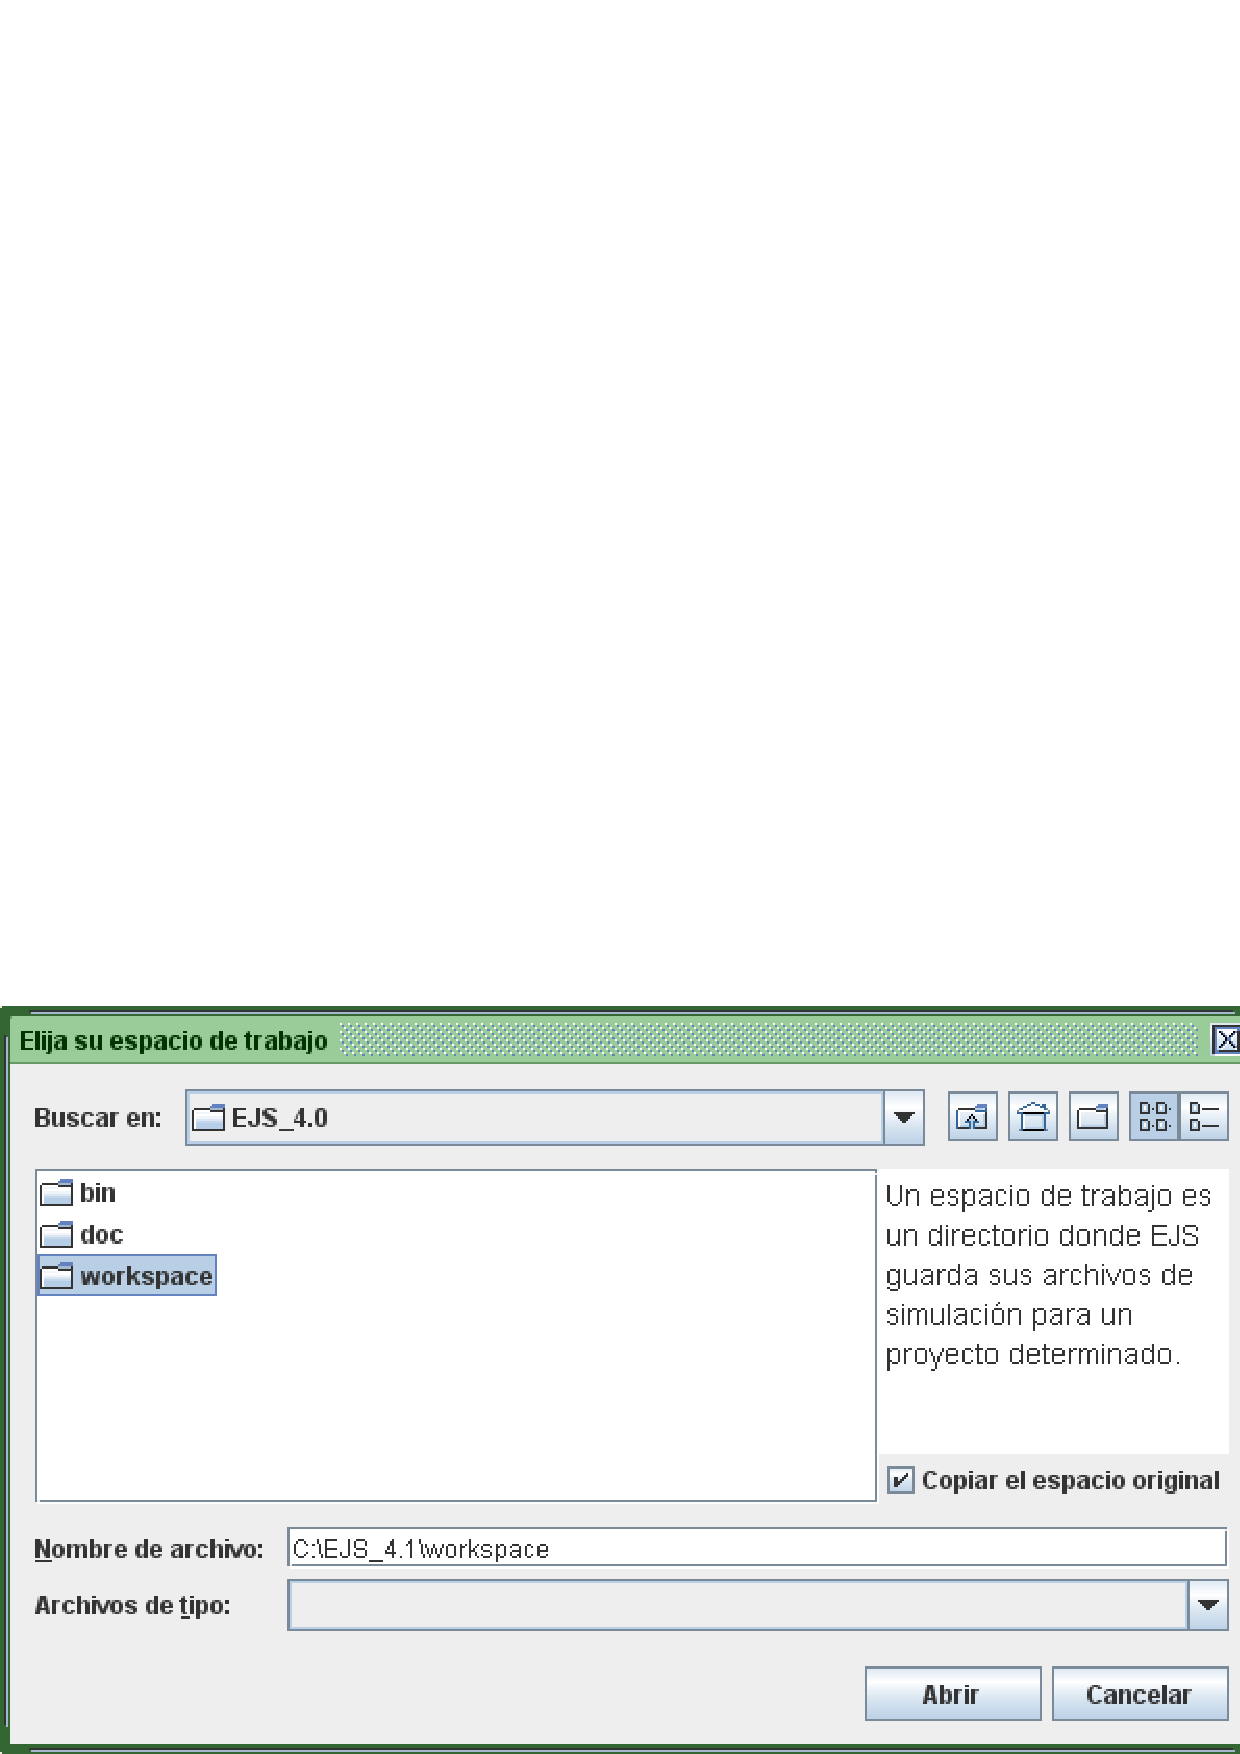
\includegraphics[scale=\scale]{01Introduction/images/WorkspaceChooser.png}
  \caption{S�lecteur de fichier pour choisir votre r�pertoire d'environnement de travail.}
  \label{fig:01Introduction/WorkspaceChooser}
\end{figure}

La console \ejs\  n'est pas une partie de \ejs, mais une utilit� qui s'utilise pour lancer un ou plusieurs exemples (copies) de \ejs\  et pour effectuer d'autres t�ches li�es � \ejs. Vous pouvez utiliser la console pour personnaliser quelques aspects de l'apparence et du fonctionnement de \ejs\ au d�marrage.~\footnote{Par exemple, fixez le \lit{look and feel} (la repr�sentation) �  \lit{CROSS\_PLATFORM}, la repr�sentation sp�cifique qui est identique sur toutes les plateformes, et lancez une nouvelle copie de \ejs\ pour appliquer le changement. Nous fixons  la repr�sentation par d�faut � \lit{SYSTEM} (syst�me), la valeur par d�faut pour votre plate-forme. Celle qui est signal�e dans ce document correspond � la repr�sentation par d�faut (appel�e \lit{Aqua}) de Mac OS X.}
La console montre aussi l'information du programme \ejs\  et les messages d'erreur sur son onglet \lit{Output area} (sortie),  auquel nous ferons r�f�rence de temps en temps dans ce document. La console cr�e un exemple de \ejs\   au d�marrage et le quitte automatiquement quand vous fermez le dernier exemple de \ejs\  en cours.
 
Cependant, avant que la console puisse ex�cuter \ejs\  juste apr�s son installation, le s�lecteur de fichier affich� sur la figure~\ref{fig:01Introduction/WorkspaceChooser}  appara�tra et vous permettra de s�lectionner dans le disque dur de l'ordinateur le r�pertoire que vous voulez utiliser comme environnement de travail (\emph{workspace}). \ejs\ utilise le concept d'environnement de travail pour organiser votre travail. Un environnement de travail est un r�pertoire dans votre disque dur sur lequel \ejs\  enregistre vos fichiers de simulation d'un projet d�termin�. Un environnement de travail peut contenir un nombre illimit� de simulations. Dans un r�pertoire d'environnement de travail, \ejs\ cr�e quatre sous-r�pertoires:\index{\Ejs!directory structure}

\begin{bulletlist}
  \item \file{config} qui est le r�pertoire pour des fichiers de configuration et des options de l'utilisateur .
  \item \file{export}  qui est le r�pertoire propos� par d�faut quand \ejs\  g�n�re des fichiers pour la distribution.
  \item \file{output} qui est le r�pertoire utilis� par \ejs\  pour placer les fichiers temporaires qui sont g�n�r�s quand vous compilez une simulation.
  \item \file{source} qui est le r�pertoire dans lequel tous les fichiers de simulation (sources et auxiliaires) doivent �tre plac�s.
\end{bulletlist}

Quand vous ex�cutez pour la premi�re fois  \ejs,  la console vous demande de choisir un r�pertoire de votre disque dur comme votre environnement de travail (\emph{workspace}). Celui-ci doit �tre un r�pertoire enregistrable n'importe o� dans votre disque dur.
 Vous pouvez d�cider d'utiliser l'environnement de travail qui est inclus dans la distribution par exemple, le r�pertoire d'environnement de travail dans le r�pertoire \file{EjsS\_X.x} qui est cr�� quand vous d�compressez le paquet \ejs. Mais il est \textbf{fortement recommand�} de cr�er un nouveau r�pertoire dans votre r�pertoire personnel habituel (ou mieux encore, un r�pertoire sur le cloud --- comme \lit{Dropbox} \link{http://dropbox.com}  ou similaire). Le dialogue de s�lection de fichier qui vous permet de choisir l'environnement de travail dispose d'une case qui, une fois coch�e, copie tous les exemples de fichiers de distribution dans le nouvel environnement de travail. Maintenez cette case coch�e et vous trouverez quelques sous-r�pertoires dans le r�pertoire \file{source} de votre environnement de travail qui contient des exemples de simulations. En particulier vous trouverez les r�pertoires \file{JavaExamples} (Exemples de Java) et \file{JavascriptExamples}  (Exemples de JavaScript) d�crits dans les chapitres ult�rieures de ce document.
  

\note{Bien que cela ne soit pas n�cessaire en g�n�ral, vous pouvez cr�er et utiliser plus d'un environnement de travail pour de diff�rents projets ou t�ches. La console pr�voit un s�lecteur qui vous permet de changer l'environnement de travail en cours et \ejs\  retiendra l'environnement de travail actuel entre les s�ances, m�me si vous r�installez \ejs.}

Finalement la premi�re fois que vous ex�cutez \ejs, le programme vous demandera d'indiquer votre nom et affiliation (Figure~\ref{fig:01Introduction/NameAndAffiliation}). Cette d�marche est optionnelle mais elle est recommand�e car elle vous aidera � documenter vos simulations futures. Vous pouvez d�cider de saisir ou de modifier cette information plus tard en utilisant l'ic�ne \lit{\ejs\ options}, 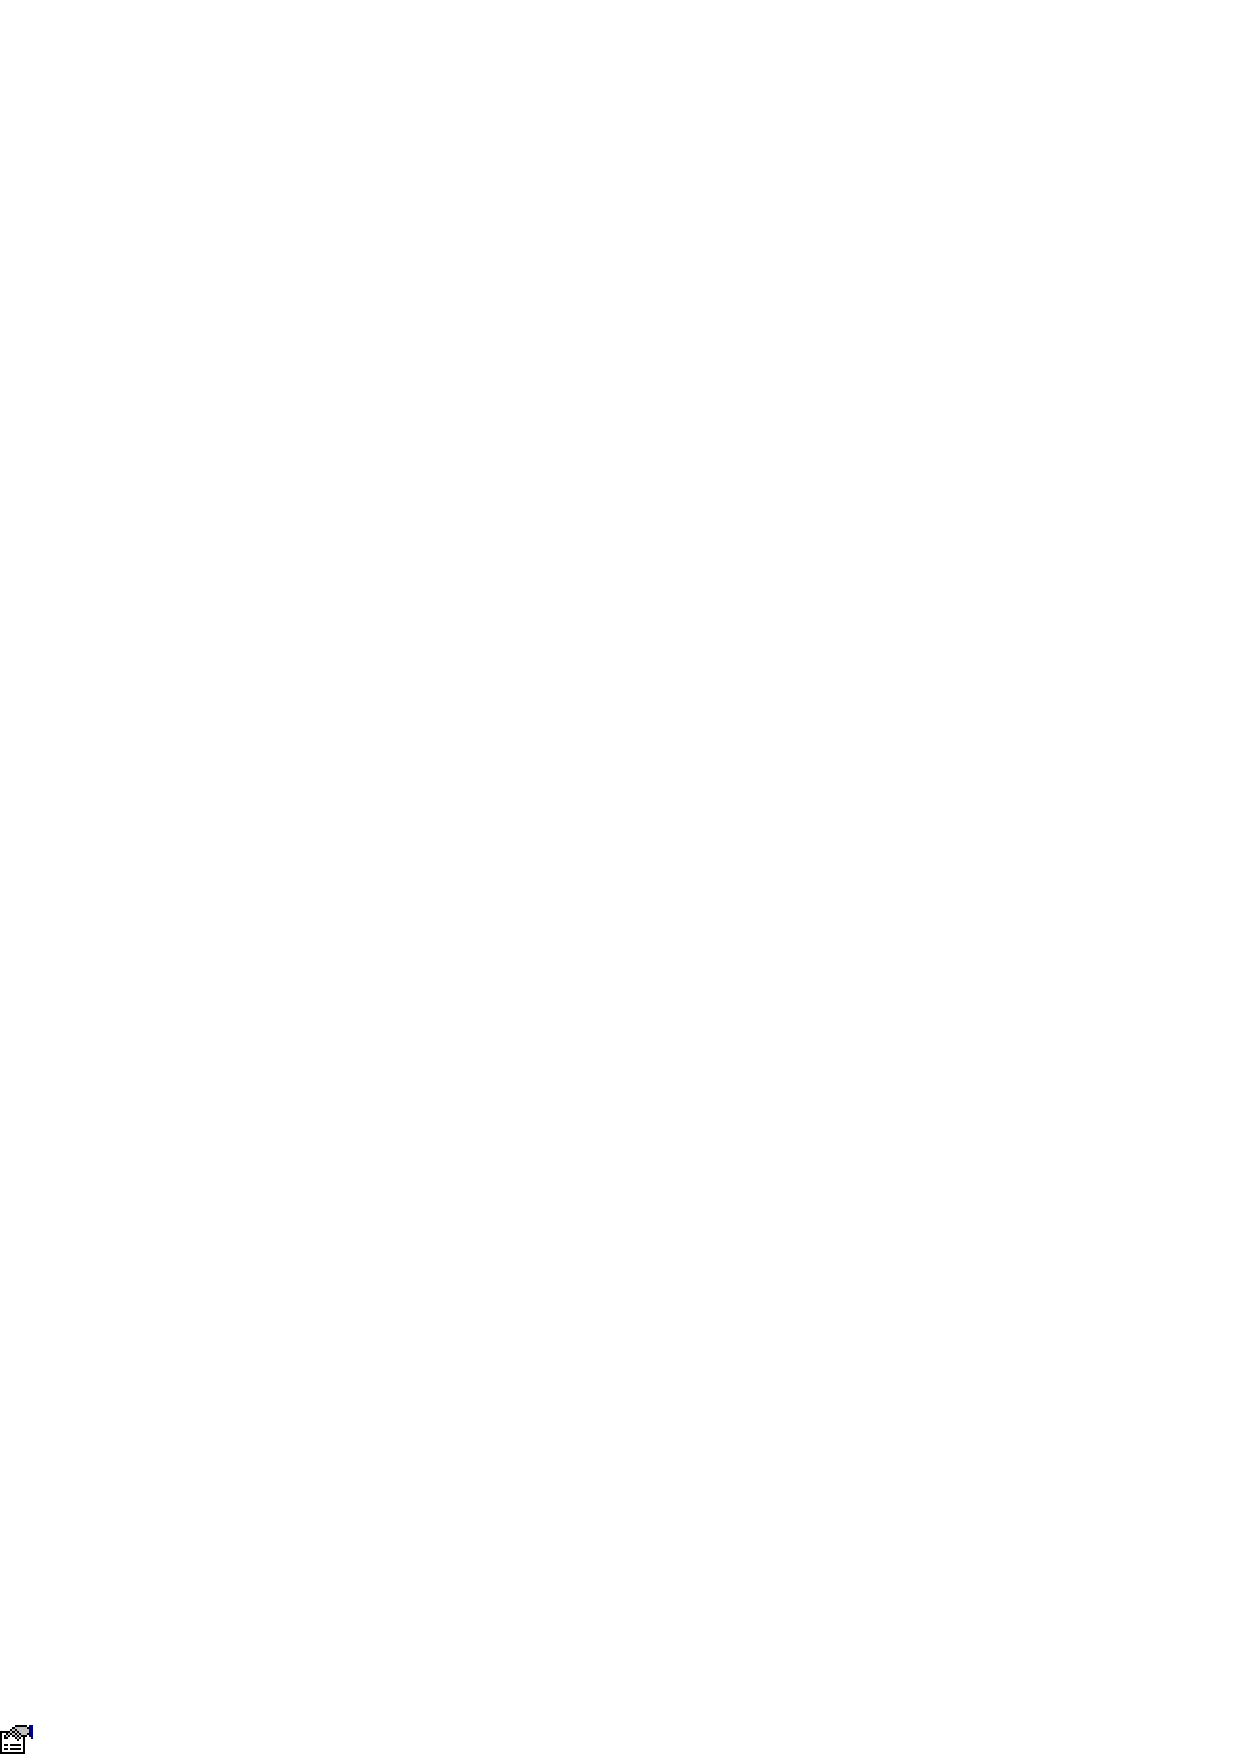
\includegraphics[scale=\linescale]{../_common/icons_png/edit.png}, de la barre des t�ches de \ejs.

\begin{figure}[htb]
  \centering
  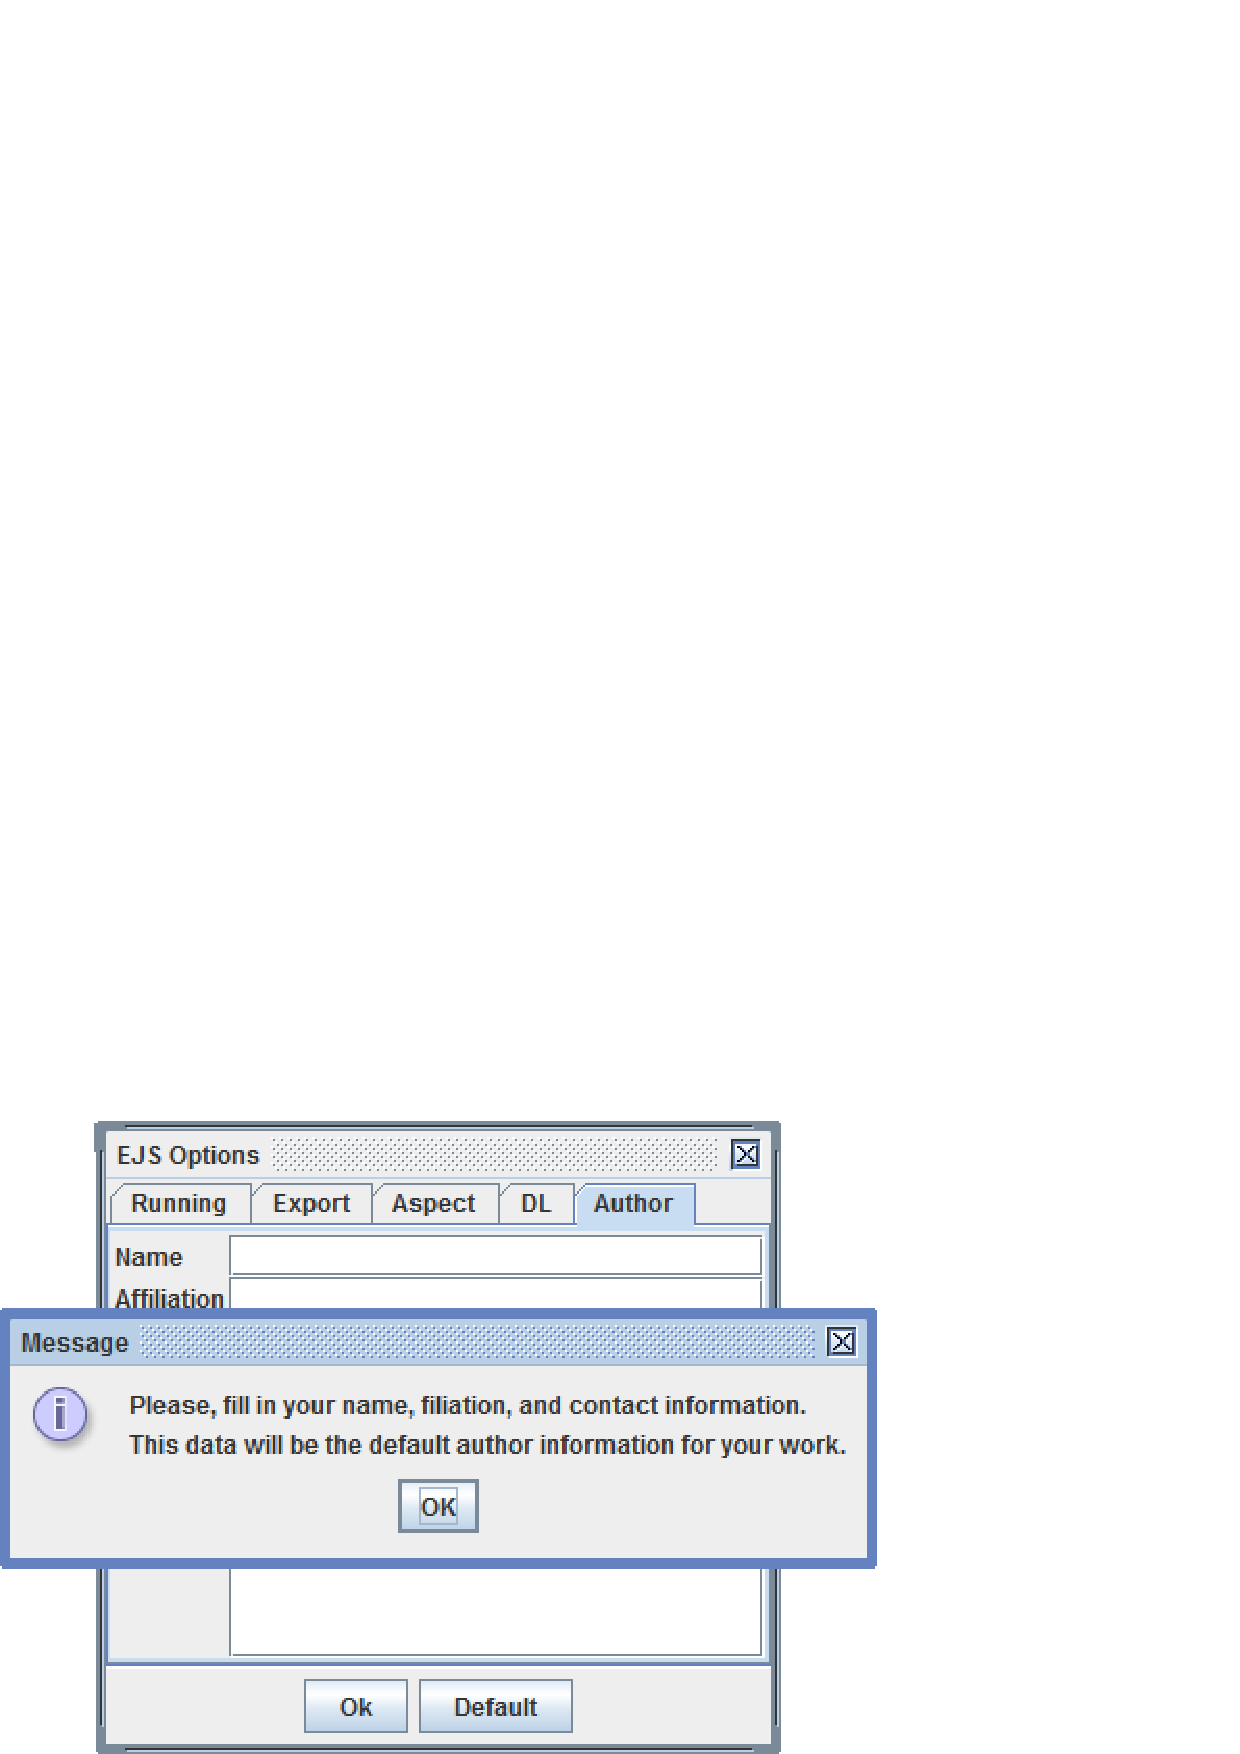
\includegraphics[scale=\scale]{01Introduction/images/NameAndAffiliation.png}
  \caption{Optionellement indiquez votre nom et affiliation.}
  \label{fig:01Introduction/NameAndAffiliation}
\end{figure}

% ------------------------
    \section{Interface graphique utilisateur}\label{section:01GUI}\index{\Ejs!graphical user interface}
% ------------------------

Vous �tes pr�t maintenant pour diriger votre attention sur l'outil de mod�lisation \ejs, affich� avec des annotations � la figure~\ref{fig:01Introduction/EjsInterface}. En d�pit de son interface simple, \ejs\  pr�sente tous les outils n�cessaires pour un cycle de mod�lisation complet.

\begin{figure}[htb]
  \centering
  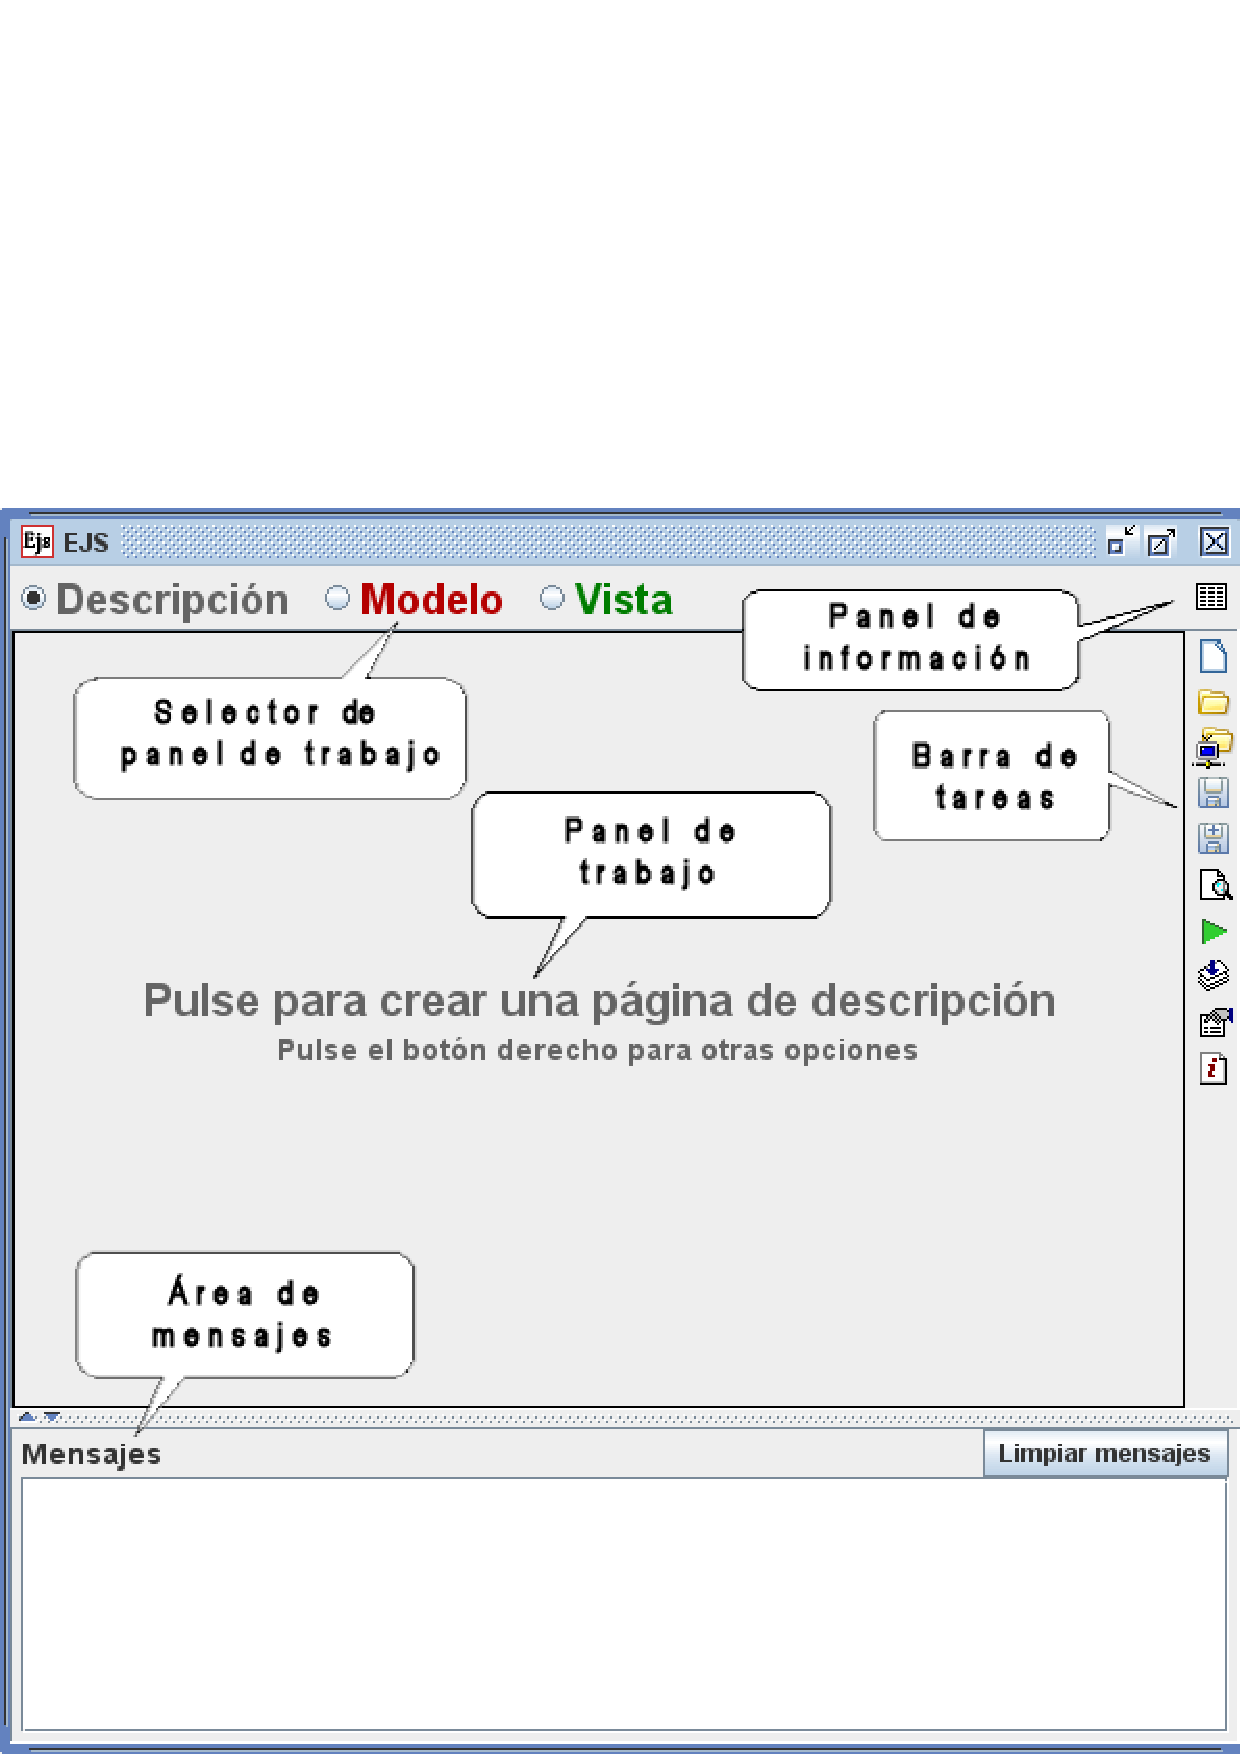
\includegraphics[scale=\scale]{01Introduction/images/EjsInterface.png}
  \caption{L'interface utilisateur de \ejs\ avec des annotations.}
  \label{fig:01Introduction/EjsInterface}
\end{figure}

La barre de t�che\index{\Ejs!taskbar} de la droite fournit une s�rie d'ic�nes pour effacer, ouvrir, rechercher et enregistrer un fichier, pour configurer \ejs, et pour afficher l'information du programme et la bulle d'aide. Elle fournit aussi des ic�nes pour ex�cuter une simulation et pour stocker une ou plusieurs simulations sur un fichier autonome. Si vous faites un clic droit sur les ic�nes de la barre de t�che, des actions alternatives (mais en relation) s'affichent, celles-ci seront d�crites en fonction de la n�cessit�. La partie inf�rieure de l'interface contient une zone de donn�es de sortie\index{\Ejs!output area}  sur laquelle  \ejs\  affiche des messages. La partie centrale de l'interface contient des panneaux (espaces) de travail sur lesquels la mod�lisation est �labor�e.


\Ejs\  fournit trois panneaux de travail pour la mod�lisation. Le premier panneau \lit{Description} nous permet de cr�er et d'�diter un texte multim�dia bas� sur HTML qui d�crit le mod�le.\index{HTML}  Chaque page qui contient un texte appara�t dans un panneau �tiquet� dans le panneau de travail et  un clic droit sur la barre �tiquet� permet � l'utilisateur d'�diter le texte ou d'importer un texte additionnel. Le deuxi�me panneau de travail, \lit{Model} (Mod�le) est d�di� au processus de mod�lisation. Nous utilisons ce panneau pour cr�er des variables qui d�crivent le mod�le, pour initialiser ces variables et pour �crire des algorithmes qui d�crivent comment ce mod�le change dans le temps. Le troisi�me panneau de travail \lit{View} (Vue) ou \lit{HtmlView} (Vue Html, pour les interfaces bas�es sur HTML5) est d�di� � la t�che d'�laborer l'interface graphique utilisateur qui permet � l'utilisateur de contr�ler la simulation et d'afficher les donn�es de sortie. Nous �laborons l'interface en s�lectionnant les �l�ments de la palette et en les ajoutant au \lit{Tree of elements} (arbre des �l�ments) de la vue. Par exemple, la palette \lit{Interface} contient des boutons, des sliders (curseurs) et des champs de saisie, et la palette  \lit{2D Drawables} contient des �l�ments pour repr�senter les donn�es en 2D.

% ------------------------
   % \subsection{Programming languages support}\label{section:02Languages}\index{\Ejs!programming languages}
% ------------------------

\Ejs\ supporte plus d'un langage de programmation pour impl�menter les algorithmes n�cessaires pour le processus de mod�lisation. L'interface pour tous ces langages est bas�e sur les m�mes principes, donc si vous apprenez � l'utiliser pour un de ces langages, vous arriverez � tous les comprendre. Quelquefois nous faisons r�f�rence � de diff�rentes interfaces de \Ejs\ pour de diff�rents langages de programmation comme  \emph{les ar�mes} de \ejs. Donc, nous pouvons, par exemple, faire r�f�rence � \emph{l'ar�me Java} ou � \emph{l'ar�me JavaScript} de \ejs .

La console \ejs\  lance, par d�faut, un exemple-copie de \ejs\  qui supporte le langage de programmation Java (c'est-�-dire un exemple de l'ar�me Java de \ejs). Vous pouvez changer le langage de programmation support� -- ou l'ar�me -- en utilisant le s�lecteur \lit{Programming language} (langage de programmation) dans la barre \lit{Basic options} de la console \ejs, et lancer un autre exemple de \ejs\  pour ce langage de programmation en cliquant le bouton \lit{Launch \ejs}. La figure~\ref{fig:01Introduction/EjsInterfaceJS} affiche  l'interface graphique utilisateur pour la cr�ation de mod�les JavaScript sur \Ejs.

\begin{figure}[htb]
  \centering
  \includegraphics[scale=\scale]{01Introduction/images/EjsInterfaceJS.png}
  \caption{L'interface utilisateur de  \Ejs\ pour le support Javascript.}
  \label{fig:01Introduction/EjsInterfaceJS}
\end{figure}

Les deux chapitres suivants de ce document vous guideront pour voir en d�tail et ex�cuter une simulation existante dans chaque langage de programmation support�. (La simulation montre le m�me ph�nom�ne physique dans tous les cas.) Cela vous aidera � comprendre comment  les panneaux  \lit{Description}, \lit{Model} et \lit{View} (ou \lit{HtmlView}) fonctionnent collaborativement pour vous aider � mod�liser une simulation. Si vous �tes d�butant sur \Ejs, veuillez lire le chapitre de l'ar�me \ejs\  qui vous int�resse le plus avant d'examiner un des mod�les existants dans notre biblioth�que num�rique.

% -----------------------------------------------------
\section{Trouver des mod�les}\label{section:01FindingModels}
% -----------------------------------------------------

Une fois que vous avez abord� les �l�ments basiques de \ejs\   et que vous savez comment t�l�charger, examiner, ex�cuter et m�me modifier un exemple, vous serez s�rement int�ress� � trouver des simulations existantes pour voir ce que d'autres utilisateurs ont fait avec \ejs. Vous trouverez peut-�tre un mod�le qui s'adapte � vos besoins ou que vous pouvez facilement modifier pour son utilisation en cours.

Il y a deux lieux que vous pouvez consulter pour trouver plus de mod�les. Le premier lieu � consulter c'est le r�pertoire exemple \file{source} qui est associ� � la distribution de \ejs. Dans le r�pertoire \file{source} de l'environnement de travail de distribution, vous trouverez quelques r�pertoires avec des exemples de simulations. Ces r�pertoires exemples ont �t� aussi copi�s sur votre propre environnement de travail (� moins que vous ayez d�sactiv� cette option) quand vous avez ex�cut� pour la premi�re fois \ejs.
	
Le deuxi�me lieu (en fait, lieux), et probablement le plus int�ressant, pour chercher des nouveaux mod�les est disponible sur Internet. L'ic�ne de la biblioth�que num�rique de \ejs\  sur la barre d'outils, 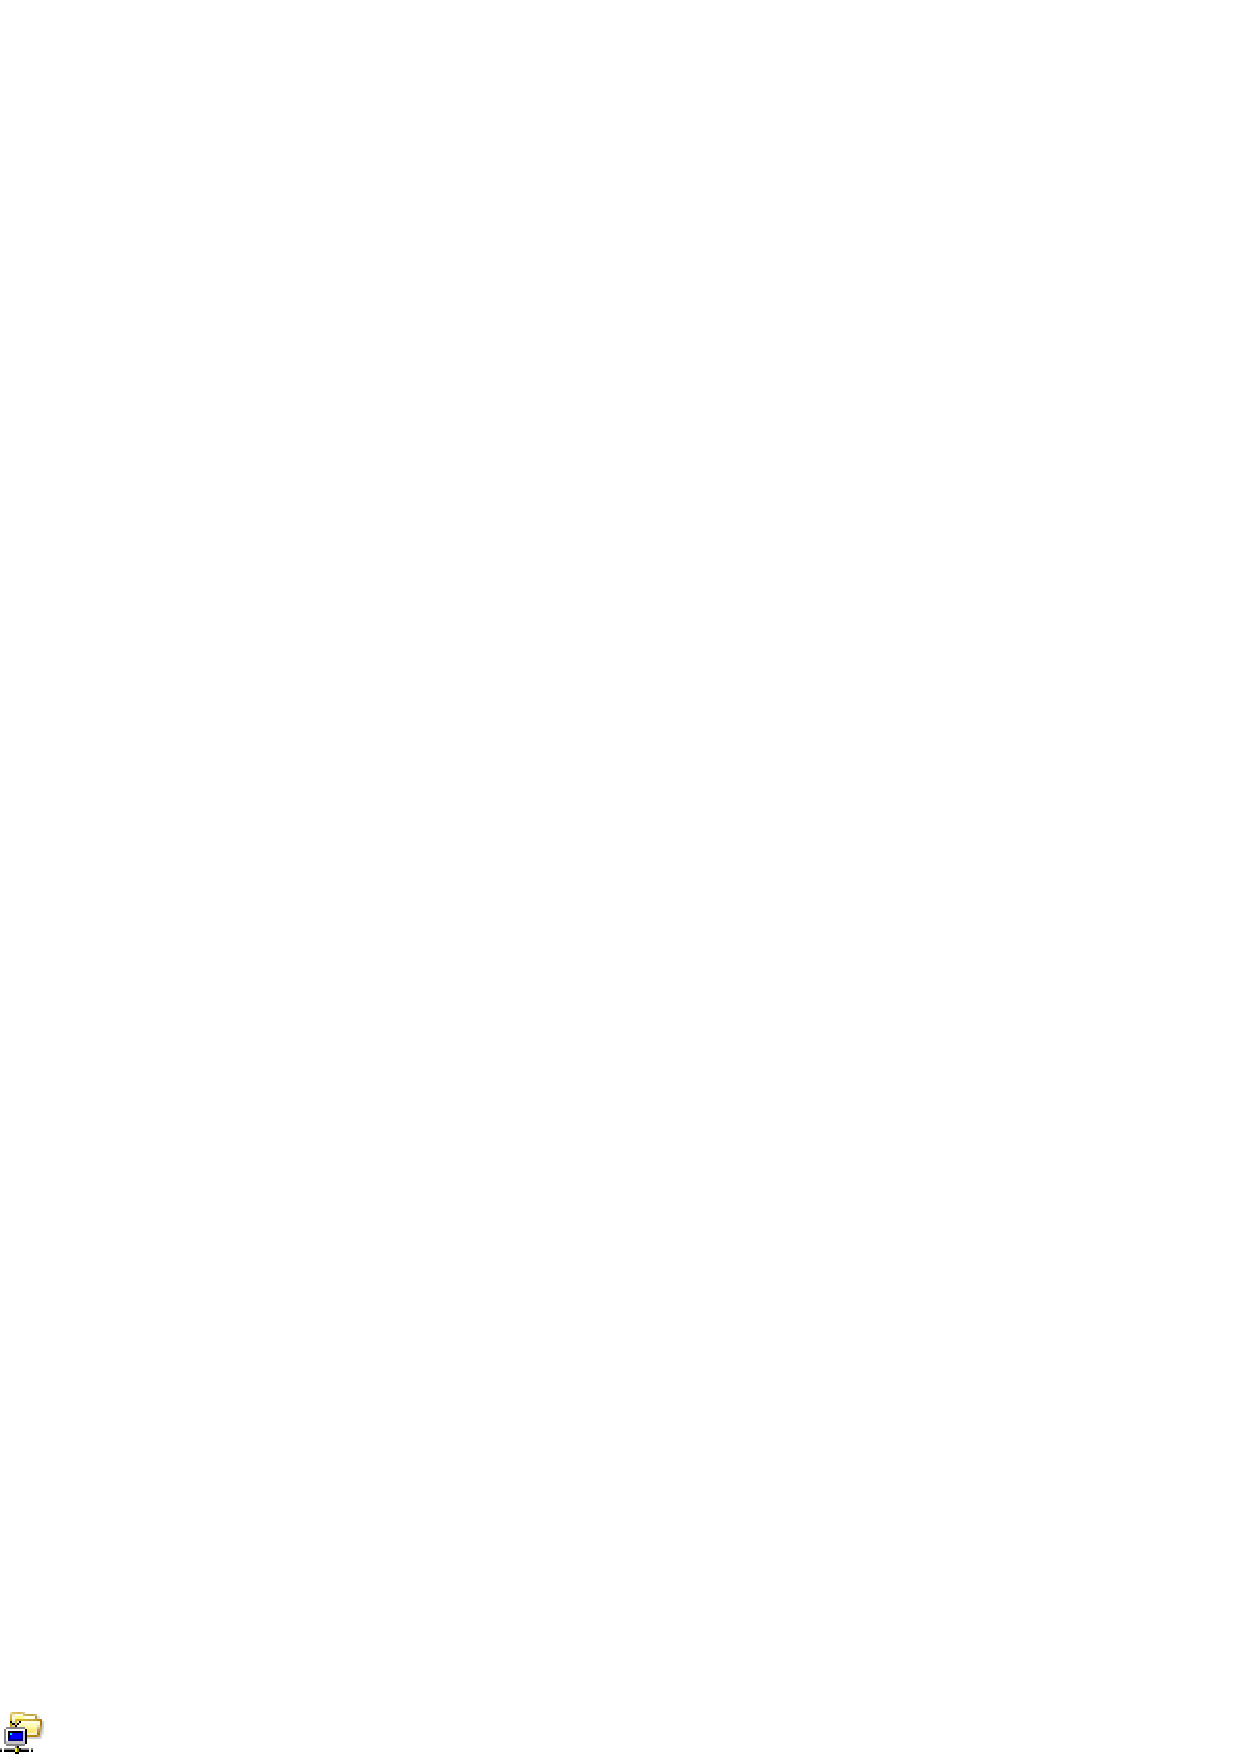
\includegraphics[scale=\linescale]{../_common/icons_png/netOpen.png}, ouvre une fen�tre qui nous permet de nous connecter � des r�f�rentiels de mod�les \ejs\  disponibles sur Internet. Cette fen�tre, affich�e dans la figure~\ref{fig:01Introduction/EJSDigitalLibraries}, contient une bo�te combin�e dans sa partie sup�rieure qui fournit une liste des biblioth�ques num�riques disponibles. Une deuxi�me bo�te combin�e vous permet de s�lectionner le langage de programmation souhait� pour les mod�les. S�lectionnez une de ces biblioth�ques, le langage de programmation ou cliquez sur le bouton \lit{Refresh} (actualiser) pour obtenir une liste des mod�les disponibles. Toutes ces biblioth�ques fonctionnent d'une mani�re similaire et nous utilisons le r�f�rentiel de biblioth�que num�rique \textbf{comPADRE} pour illustrer comment nous y acc�dons sur \ejs.

\begin{figure}[htb]
    \centering
  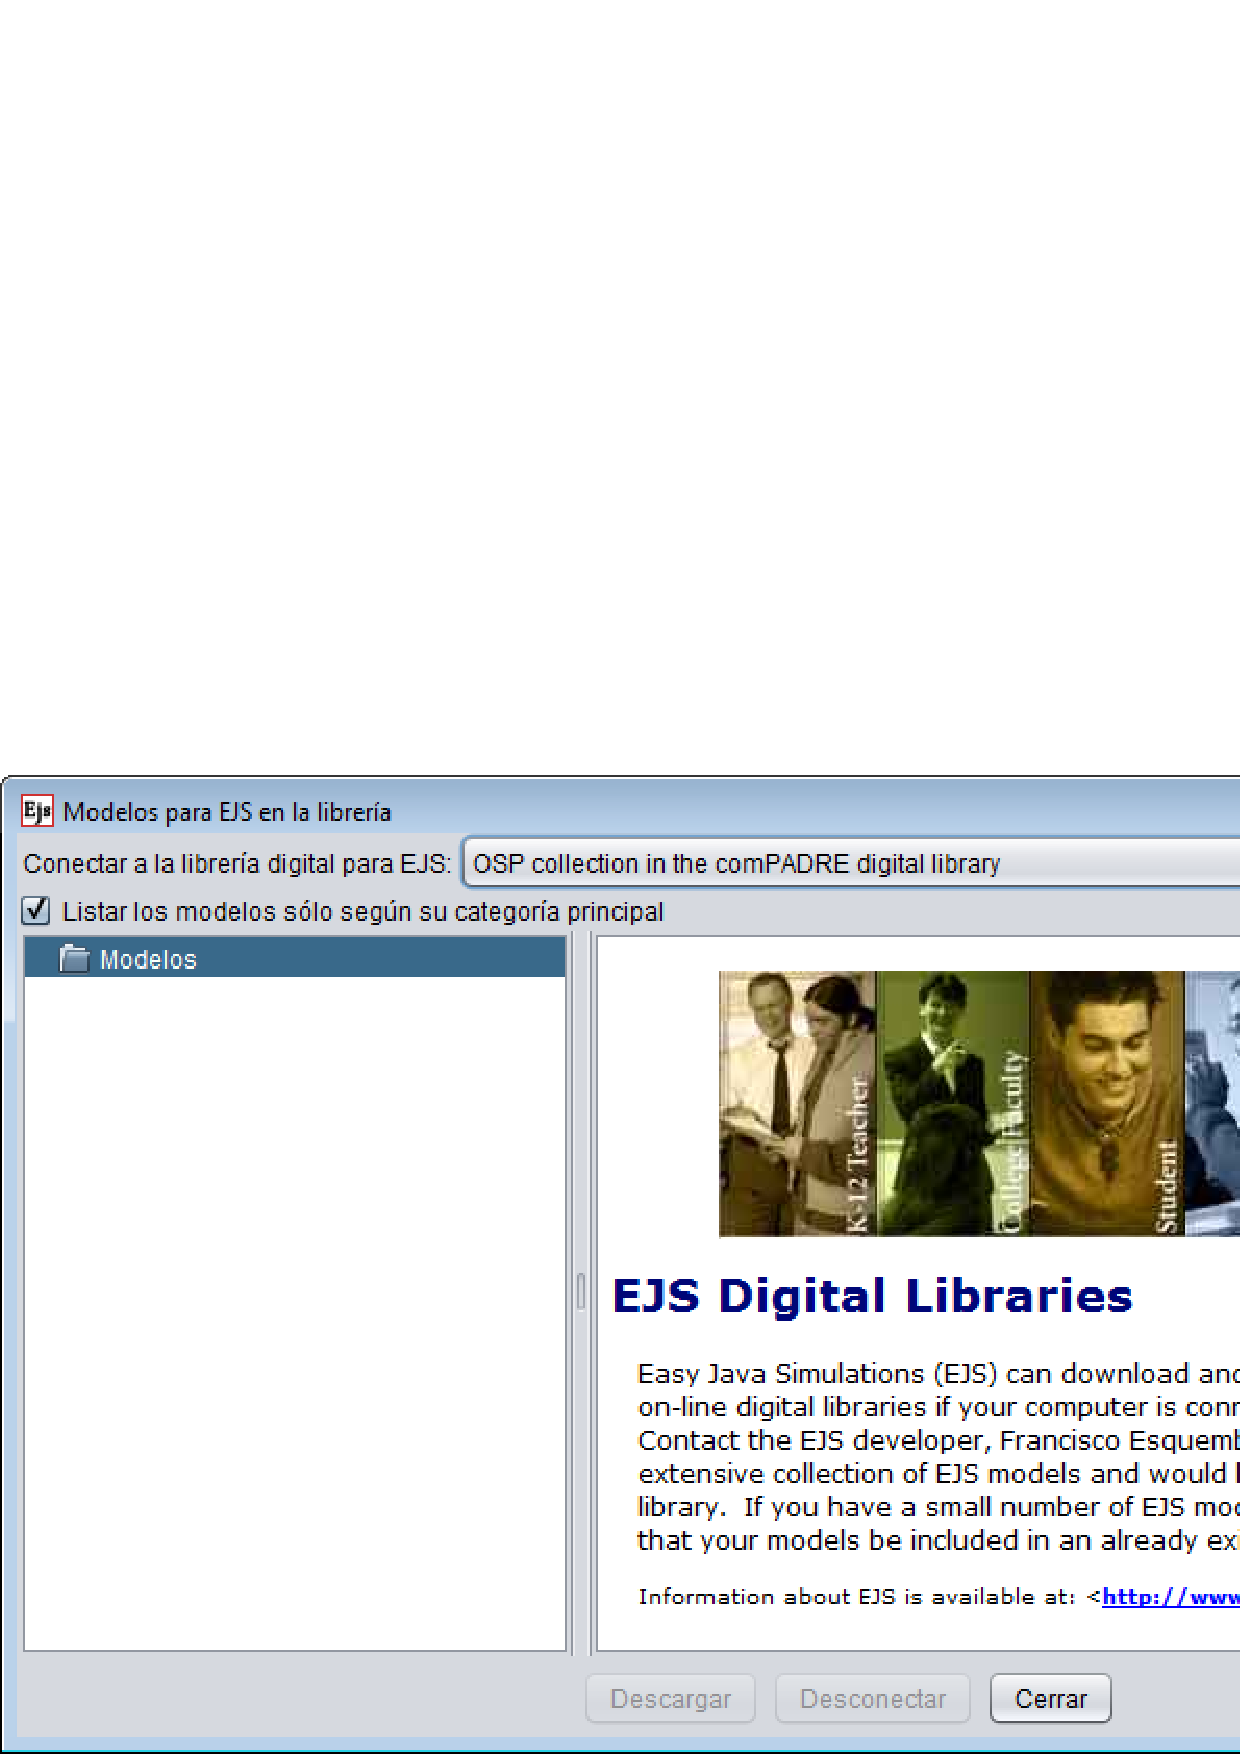
\includegraphics[scale=\scale]{01Introduction/images/EJSDigitalLibraries.png}
    \caption{La fen�tre de biblioth�que num�rique de \ejs. S�lectionnez un des r�f�rentiels disponibles en utilisant la bo�te combin�e dans la partie sup�rieure de la fen�tre, le langage de programmation souhait� ou cliquez sur le bouton \lit{Refresh} pour obtenir la liste des mod�les disponibles.}
    \label{fig:01Introduction/EJSDigitalLibraries}
\end{figure}

Le \textbf{comPADRE Pathway} (sentier \emph{comPADRE}), qui est une partie de la Biblioth�que Nationale Num�rique de Sciences des �tats-Unis, est un r�seau en expansion de collections de ressources �ducatives con�u pour venir en aide aux enseignants et aux �tudiants de physique et en astronomie.  De sp�ciale relevance pour nos int�r�ts, c'est la collection Open Source Physics (OSP) --- physique de  source ouverte --- de comPADRE, disponible sur \link{http://www.compadre.org/OSP}. Cette collection contient des ressources informatiques pour l'enseignement sous forme de simulations ex�cutables et des ressources p�dagogiques qui attire l'attention des �tudiants vers la physique, le calcul num�rique et la mod�lisation informatique. En particulier, elle contient des mod�les auxquels nous pouvons acc�der � travers de leurs codes source (XML)  directement � partir de \ejs\  en utilisant l'ic�ne de biblioth�ques num�riques.

Si vous �tes connect� � Internet, s�lectionnez la saisie \lit{OSP collection on the comPADRE digital library}  (la collection OSP de la biblioth�que num�rique comPADRE) de la bo�te combin�e sup�rieure et  \ejs\   vous connectera � la biblioth�que pour obtenir le tout dernier catalogue des mod�les \ejs\  de la biblioth�que. Au moment de r�diger ce document, il y avait plus de 500 mod�les Java et de 200 mod�les JavaScript organis�s dans de diff�rentes cat�gories et sous-cat�gories et on estime que la collection devrait augmenter. Comme nous indique le cadre de gauche de la figure~\ref{fig:01Introduction/OSPCollection} la collection est organis�e en cat�gories et sous-cat�gories. Quand le nom d'une sous-cat�gorie appara�t en rouge, faites un double clic pour ouvrir le n\oe{}ud avec la liste des mod�les de la sous-cat�gorie. Comme beaucoup de mod�les ont une classification primaire et secondaire, une case � cocher dans le volet sup�rieur � c�t� du champ de recherche (\lit{Search}) vous permet de d�cider si vous voulez que les mod�les soient �num�r�s uniquement sous leur classification primaire ou qu'ils apparaissent dans toutes les cat�gories correspondantes (dans ce cas ils appara�tront plus d'une fois)

\begin{figure}[htb]
    \centering
  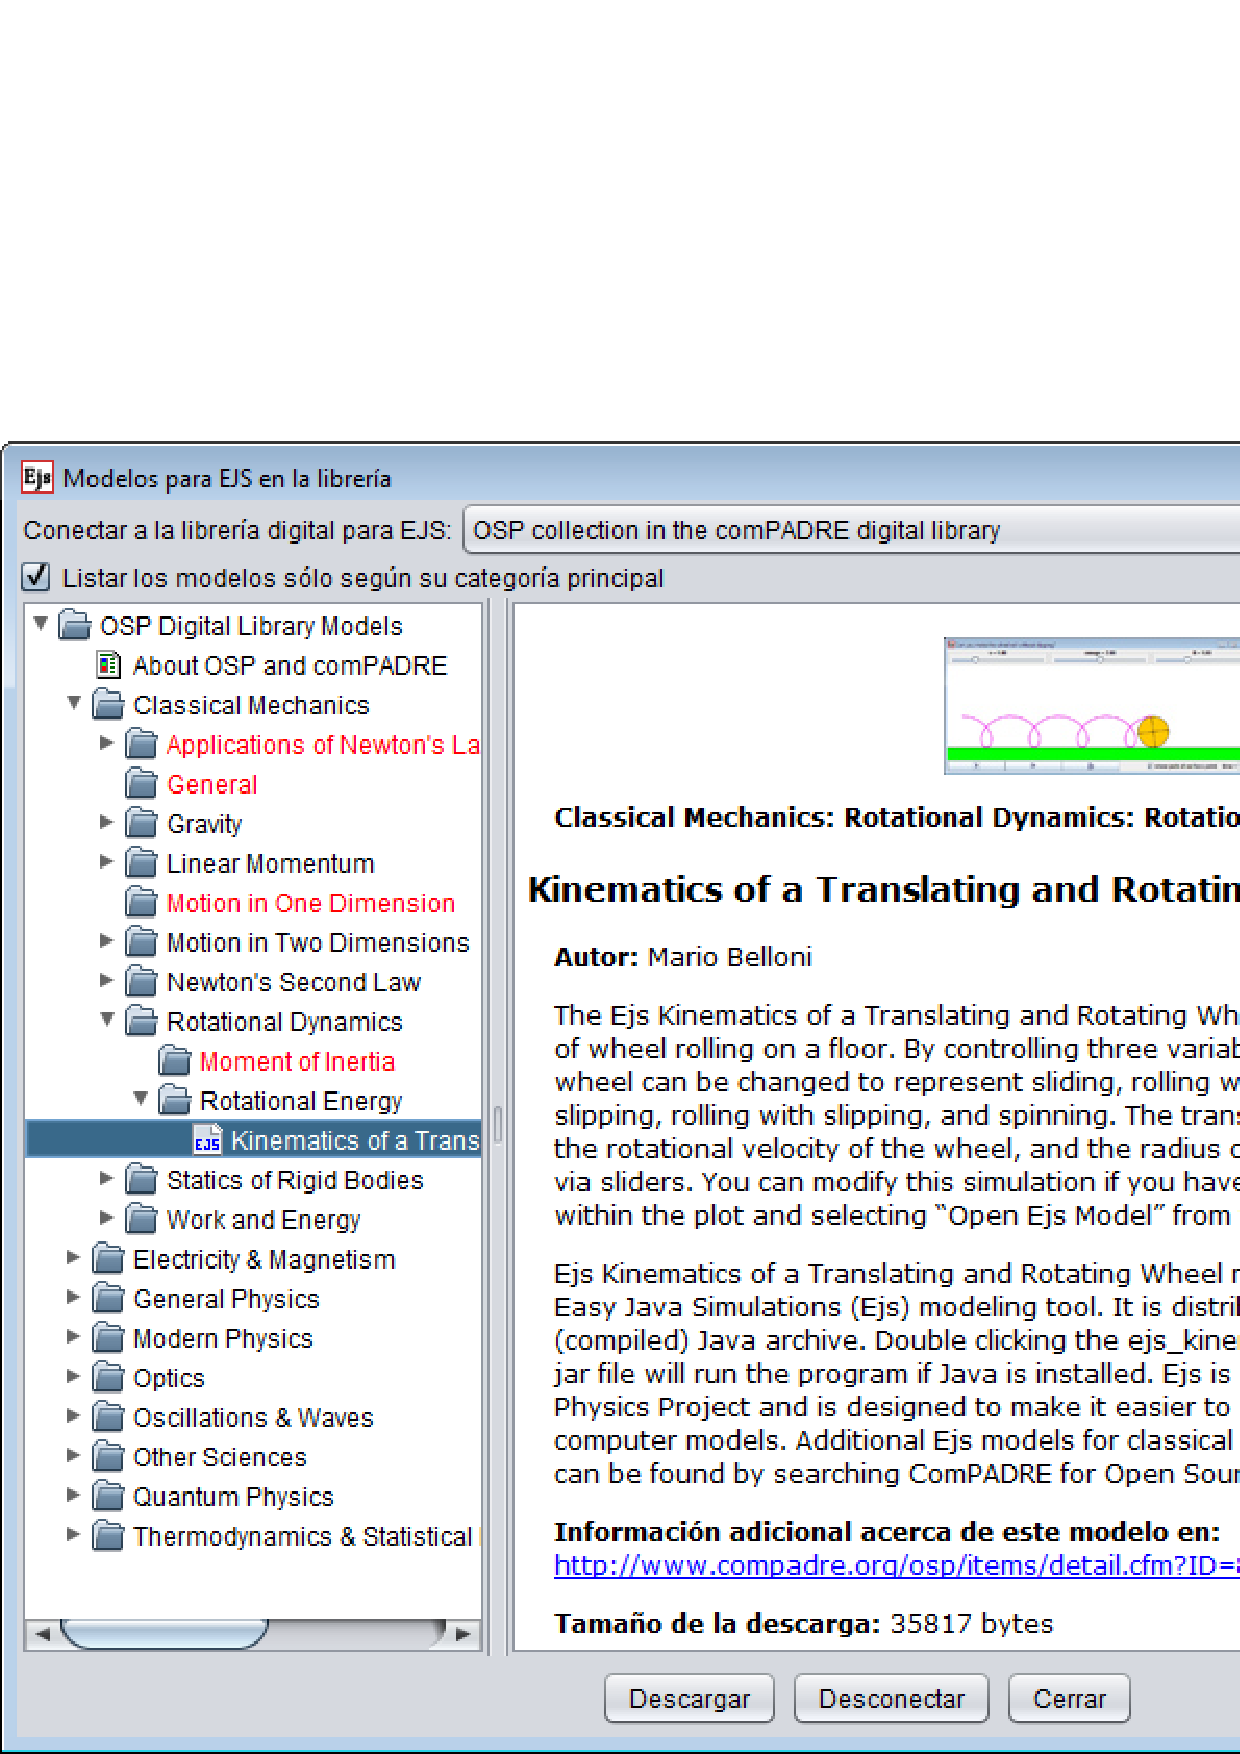
\includegraphics[scale=\scale]{01Introduction/images/OSPCollection.png}
    \caption{La collection OSP de la biblioth�que num�rique comPADRE. Cette collection est organis�e en cat�gories et sous-cat�gories. La saisie pour un mod�le vous fournit de l'information sur le mod�le.}
    \label{fig:01Introduction/OSPCollection}
\end{figure}

Quand vous cliquez sur un n\oe{}ud mod�le, le cadre de droite vous affiche l'information sur le mod�le obtenu instantan�ment de la biblioth�que. L'information d�crit le mod�le et inclut un lien direct � la biblioth�que comPADRE pour des informations suppl�mentaires. Faites double clic sur l'entr�e du mod�le ou cliquez le bouton \lit{Download} pour extraire le mod�le et les fichiers auxiliaires de la biblioth�que,  on vous demandera un emplacement dans votre r�pertoire \file{source} de votre environnement de travail pour les  t�l�charger, et d�couvrira le mod�le sur \ejs\ quand le t�l�chargement est compl�t�. Comme les fichiers sources sont normalement petits, le t�l�chargement se fera d'une mani�re presque imm�diate. Maintenant vous pouvez examiner, ex�cuter, modifier le mod�le tel que signal� dans les chapitres d'exploration ci-dessous pour le mod�le de masse-ressort.

La collection OSP de la biblioth�que num�rique comPADRE est fortement recommand�e pour chercher des mod�les  \ejs\  et du mat�riel p�dagogique d'accompagnement.

% -----------------------------------------------------
\section{R�sum�}\label{section:02Review}
% -----------------------------------------------------

\Ejs\ est un outil de mod�lisation et d'�dition-cr�ation express�ment d�di� � la cr�ation de simulations informatiques pour �tudier et afficher une grande vari�t� de ph�nom�nes qui vont du plus simples au plus complexes. Ces simulations informatiques sont utilis�es pour obtenir des donn�es num�riques � partir de nos mod�les en fonction de la progression dans le temps et pour  montrer ces donn�es d'une mani�re que l'�tre humain puisse les comprendre. 

\ejs\  a �t� con�u pour nous permettre de travailler � un haut niveau conceptuel, pour concentrer la plupart de notre temps aux aspects scientifiques de notre simulation et demander � l'ordinateur de r�aliser automatiquement toutes les t�ches n�cessaires mais qui sont facilement automatis�es. 
Chaque outil, y compris \ejs,  pr�sente une courbe d'apprentissage. Le reste de ce document contient une s�rie d'exemples  d�taill�s qui vous permettront de vous familiariser avec les possibilit�s de mod�lisation, visualisation et interaction de EjsS.

 La mod�lisation est une science et un art. \Ejs\ est un outil qui vous permet d'exprimer vos connaissances en sciences en vous facilitant les techniques n�cessaires de l'art, et en vous fournissant un acc�s simple a beaucoup d'exemples de mod�lisation cr��s par d'autres auteurs.

          % Chapter: Introduction to Ejs
 
      % !TEX root = ../Guide de l'utilisateur de EjsS.tex

\chapter{Exploring the Java flavor of \Ejs}\label{chapter:JavaEJS}

\begin{quote}
A good example is the best sermon.  {\em Benjamin Franklin}
\end{quote}

To  provide a perspective of the modeling process, in this chapter we first load, inspect, and run an existing simple harmonic oscillator simulation. We then modify the simulation to show how \ejs\ engages the user in the modeling process and greatly reduces the amount of
programming that is required. This chapter uses Java as the programming language for the modeling and is a twin chapter of Chapter~\ref{chapter:JavascriptEJS} (where Javascript is used).

% ------------------------
    \section{Inspecting the Simulation}\label{section:02ExplorationJavaInspecting}\index{\Ejs!inspecting a simulation}
% ------------------------

As mentioned in Chapter~\ref{chapter:EjsIntro}, \Ejs\ provides three workpanels for modeling. The first panel, \lit{Description}, allows us to create and edit multimedia HTML-based narrative that describes the model.\index{HTML} 
The second work panel, \lit{Model}, is dedicated to the modeling process. We use this panel to create
variables that describe the model, to initialize these variables, and to write algorithms that describe how this model
changes in time. The third workpanel, \lit{View}, is dedicated to the task of building the graphical user interface,
which allows users to control the simulation and to display its output.  

To understand how the \lit{Description}, \lit{Model}, and \lit{View} workpanels work together, we inspect and run an
already existing simulation. Screen shots are no substitute for a live demonstration, and you are encouraged to follow along on your computer as you read.

\begin{figure}[htb]
  \centering
  \subfigure{\includegraphics[scale=0.2]{02ExplorationJava/images/OpenDialogCrossPlatform.png}}
  \subfigure{\includegraphics[scale=0.2]{02ExplorationJava/images/OpenDialogNative.png}}  
  \caption{The open file dialog lets you browse your hard disk and load an existing simulation. The appearance of the dialog 
  (shown here using two different look and feels) may vary, depending on your operating system and the selected \lit{look and feel}.}
  \label{fig:02ExplorationJava/OpenDialog}
\end{figure}

Click on the \lit{Open} icon 
\includegraphics[scale=\linescale]{../_common/icons_png/openSmall.png} on the \ejs\ taskbar. A file dialog
similar to that in Figure~\ref{fig:02ExplorationJava/OpenDialog} appears showing the contents of your workspace's \file{source}
directory. Go to the \file{JavaExamples} directory, where you will find a
file called \file{MassAndSpring.ejs}. Select this file and click on the \lit{Open} button of the
file dialog.

Now, things come to life! \ejs\ reads the \file{MassAndSpring.ejs} document which populates the workpanels and two new
``Ejs windows'' appear in your display as shown in Figure~\ref{fig:02ExplorationJava/SpringInterface}. A quick warning. You
can drag objects within these mock-up windows but this will set the model's initial conditions.  It is usually better
to set initial conditions using a table of variables as described in Section~\ref{section:02ExplorationJavaModel}.

\begin{figure}[htb]
  \centering
  \subfigure{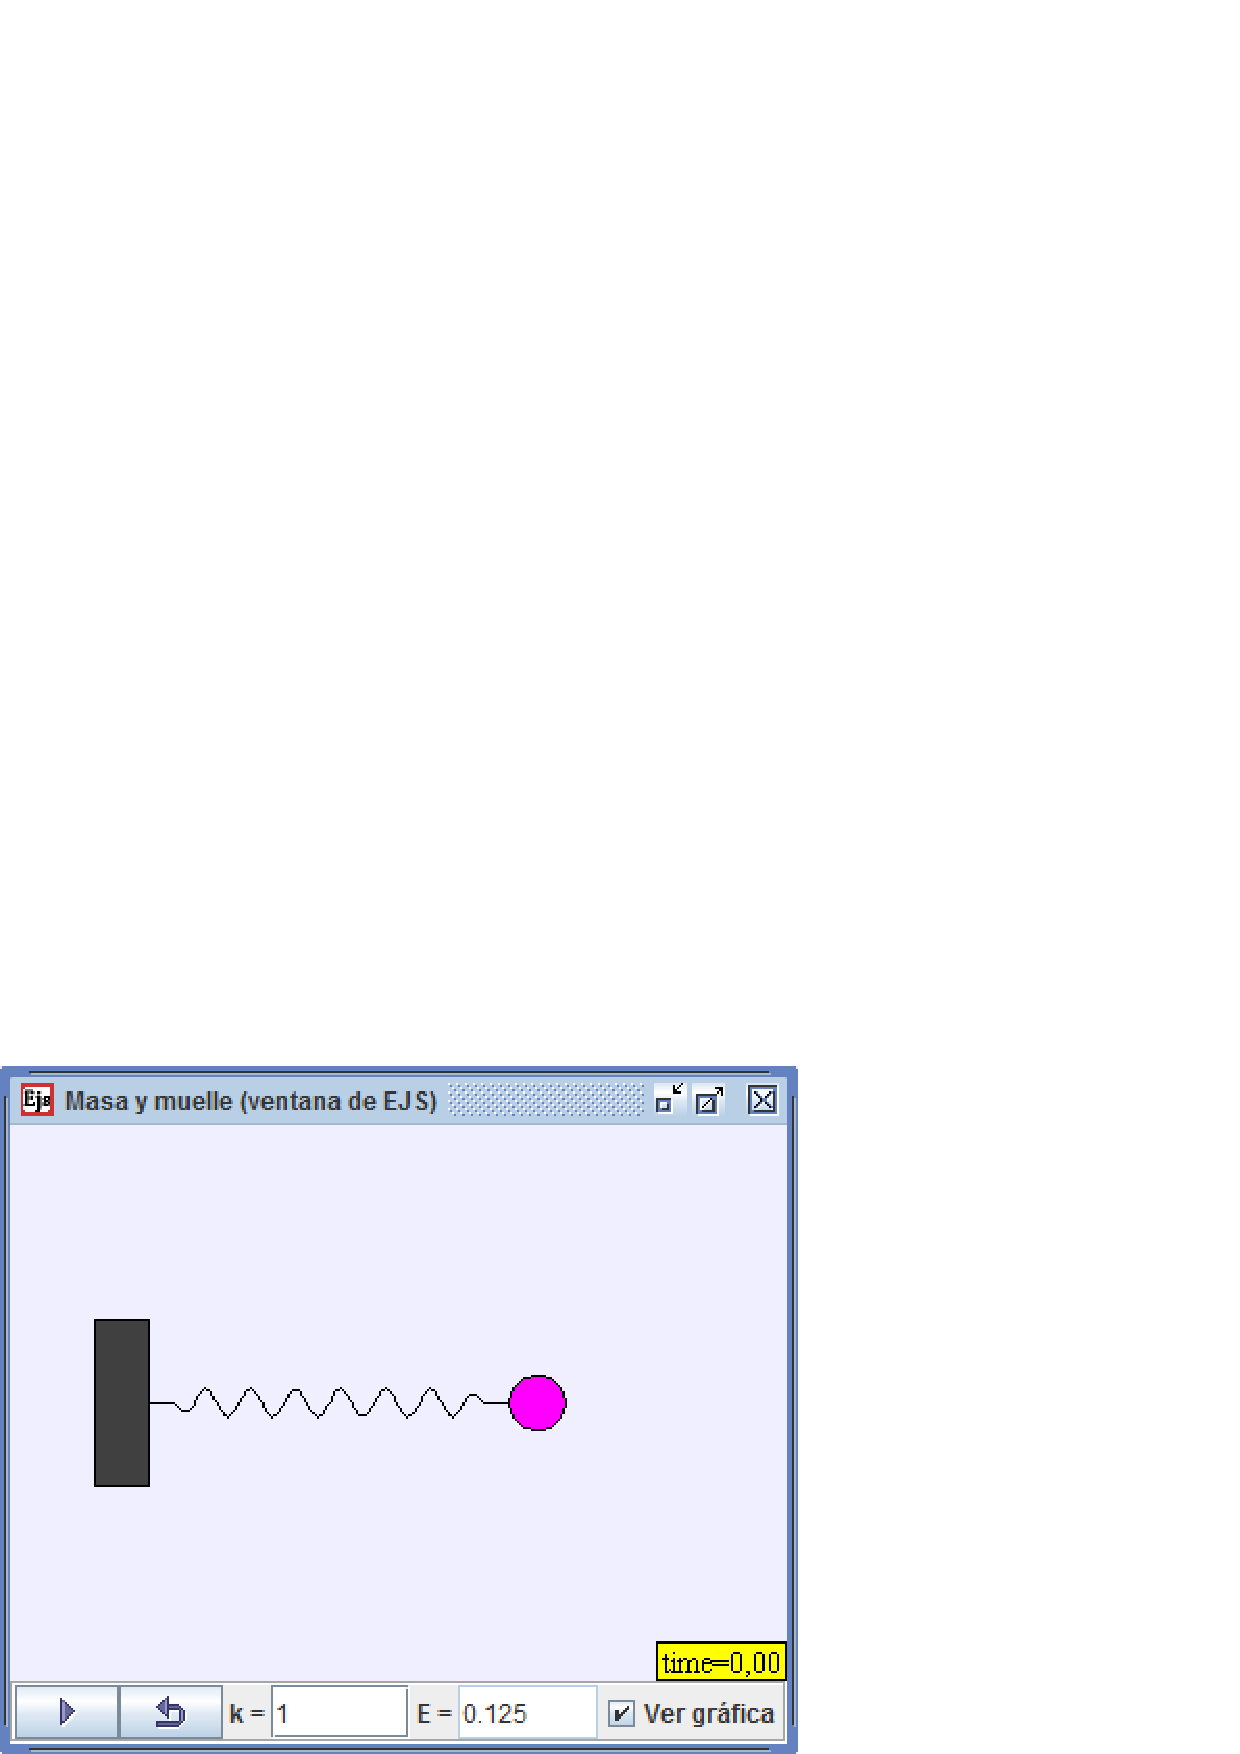
\includegraphics[scale=\scale]{02ExplorationJava/images/SpringInterface1.png}}
  \subfigure{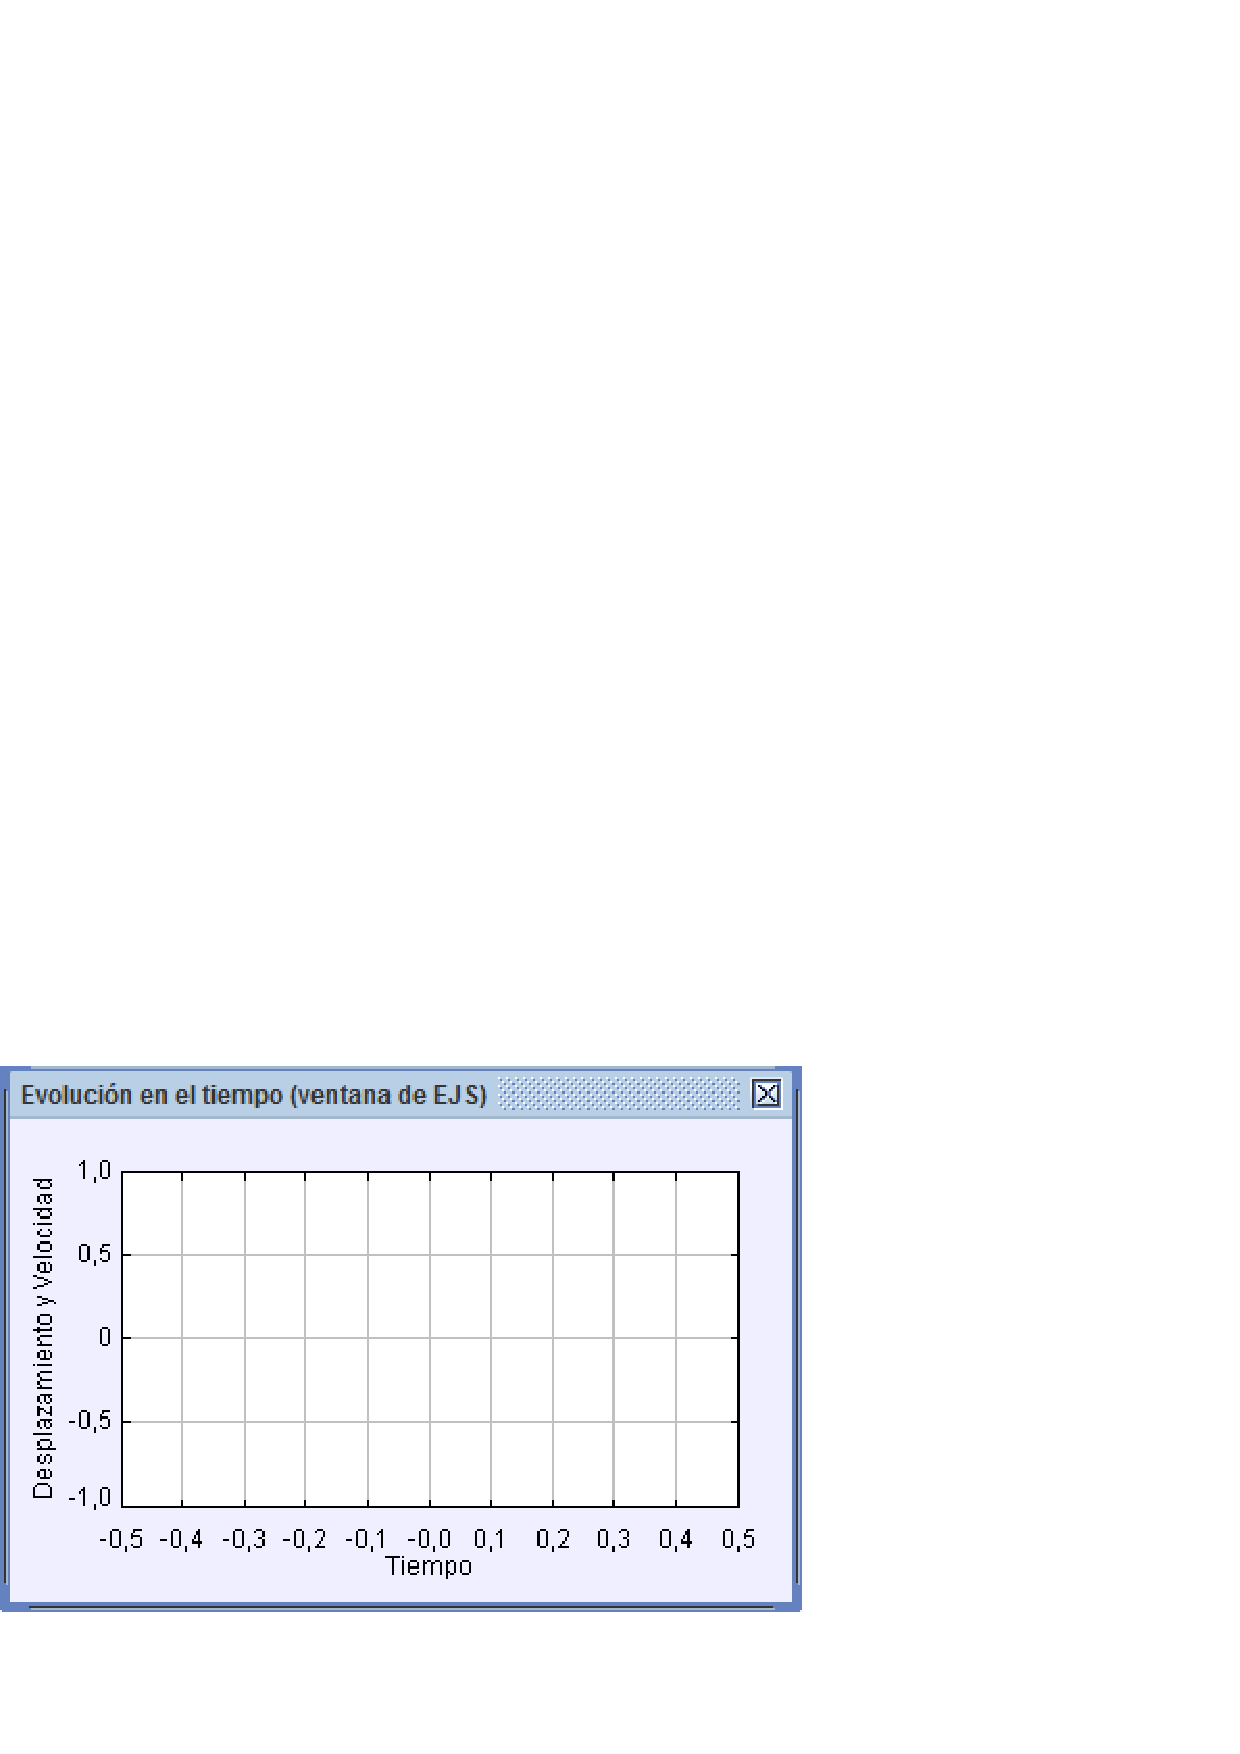
\includegraphics[scale=\scale]{02ExplorationJava/images/SpringInterface2.png}}
  \caption{\ejs\ mock-up windows of the \file{MassAndSpring} simulation. The title bar and the red border show that they are \ejs' windows
  and that the program is not running.}
  \label{fig:02ExplorationJava/SpringInterface}
\end{figure}

\note{Impatient or precocious readers may be tempted to click on the green run icon 
\includegraphics[scale=\linescale]{../_common/icons_png/launch.png} on the taskbar to execute our
example before proceeding with this tutorial.  Readers who do so will no longer be interacting with \ejs\  but with a compiled and running Java program.  Exit the running program by closing the \lit{Mass and Spring} window or by right clicking on the (now) red-squared stop icon \includegraphics[scale=\linescale]{../_common/icons_png/stop.png} on \ejs' taskbar before proceeding.}

\subsection{The \lit{Description} workpanel}

Select the \lit{Description}\index{Ejs!Description} workpanel by clicking on the corresponding radio button at the top of
\ejs, and you will see two pages of narrative for this simulation. The first page, shown in
Figure~\ref{fig:02ExplorationJava/SpringDesc}, contains a short discussion of the mass and spring model. Click on the
\lit{Activities} tab to view the second page of narrative.

\begin{figure}[htb]
  \centering
  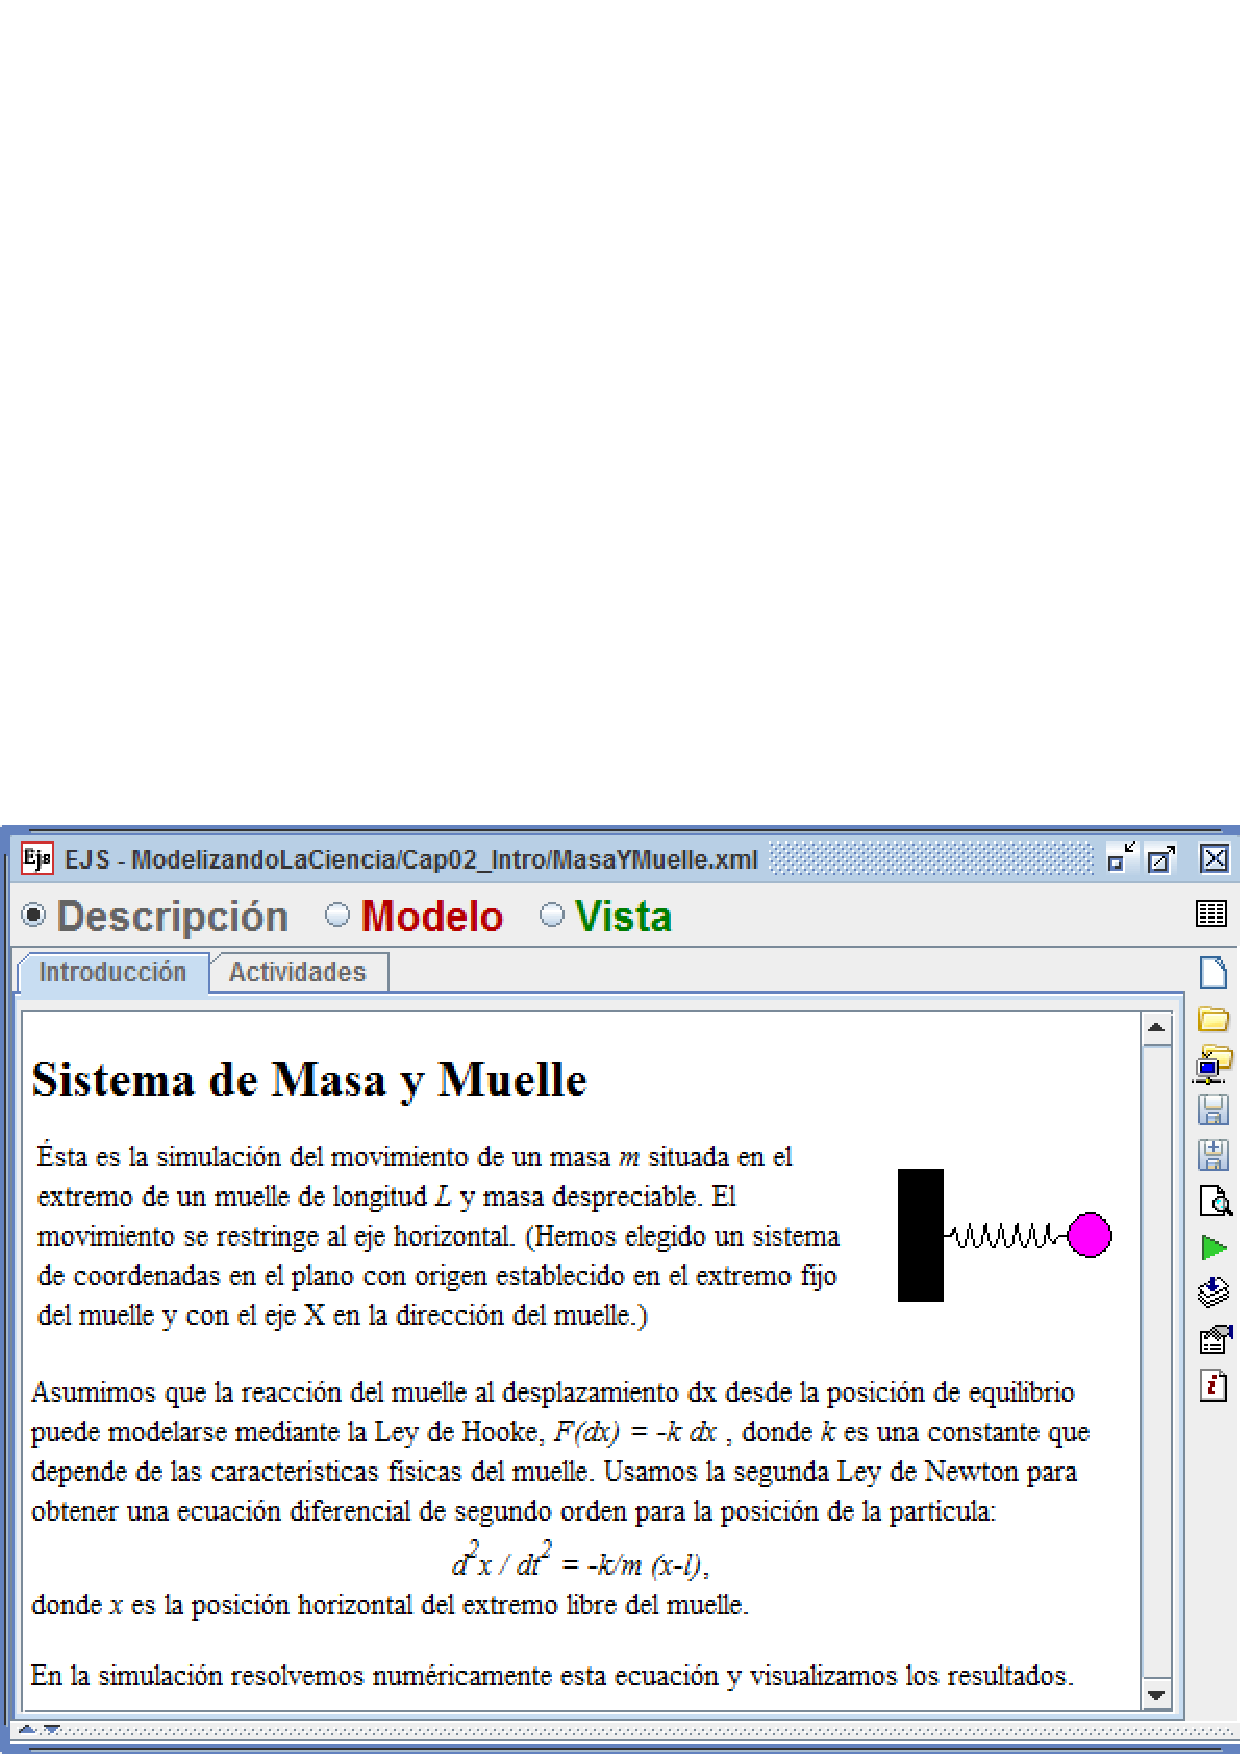
\includegraphics[scale=\scale]{02ExplorationJava/images/SpringDesc.png}
  \caption{The description pages for the mass and spring simulation. Click on a tab to display the page. Right-click on a tab to edit the page.}
  \label{fig:02ExplorationJava/SpringDesc}
\end{figure}

A \lit{Description} is HTML\index{HTML} or XHTML\index{XHTML} multimedia text that provides information and instructions about the
simulation. HTML stands for HyperText Markup Language and is the most commonly used protocol for formatting and
displaying documents on the Web. The X in XHTML stands for eXtensible. XHTML is basically HTML expressed as valid XML or, in simpler words, perfectly formatted HTML.

\ejs\ provides a simple HTML editor that lets you create and modify pages within \ejs.
You can also import HTML or (preferably) XHTML pages into \ejs\ by right clicking on a tab in the \lit{Description} workpanel. (See
Section~\ref{section:02ExplorationJavaModifyingDescription}.) Description pages are an essential part of the modeling process and
these pages are included with the compiled model when the model is exported for distribution.

\subsection{The \lit{Model} workpanel}\label{section:02ExplorationJavaModel}

The \lit{Model} workpanel is where the model is defined so that it can be converted into a program by \ejs. In this simulation,
we study the motion of a particle of mass $m$ attached to one end of a massless spring of equilibrium length $L$.
The spring is fixed to the wall at its other end and is restricted to move in the horizontal direction. Although the
oscillating mass has a well known analytic solution, it is useful to start with a simple harmonic oscillator model so that
our output can be compared with an exact analytic result.\index{Simple Harmonic Motion}

Our model assumes small oscillations so that the spring responds to a given (horizontal) displacement $\delta x$ from
its equilibrium length $L$ with a force given by Hooke's law,\index{Hooke's law} $F_x = - k \,\delta x$, where $k$ is
the elastic constant of the spring, which depends on its physical characteristics. We use Newton's second
law\index{Newton's second law} to obtain a second-order differential equation for the position of the particle:
\begin{equation}
  \frac{d^2\ x}{dt^2} = -\frac{k}{m}\,(x-L). \label{eq:02ExplorationJava/SpringBasic}
\end{equation}
Notice that we use a system of coordinates with its $x$-axis along the spring and with its origin at the
spring's fixed end. The particle is located at $x$ and its displacement from equilibrium $\delta x=x-L$ is zero when $x=L$. We solve this system numerically to study how the state evolves in time.

Let's examine how we implement the mass and spring model by selecting the \lit{Model} radio button and examining each of
its six panels.

\subsubsection{Declaration of variables}
\begin{figure}[htb]
    \centering
  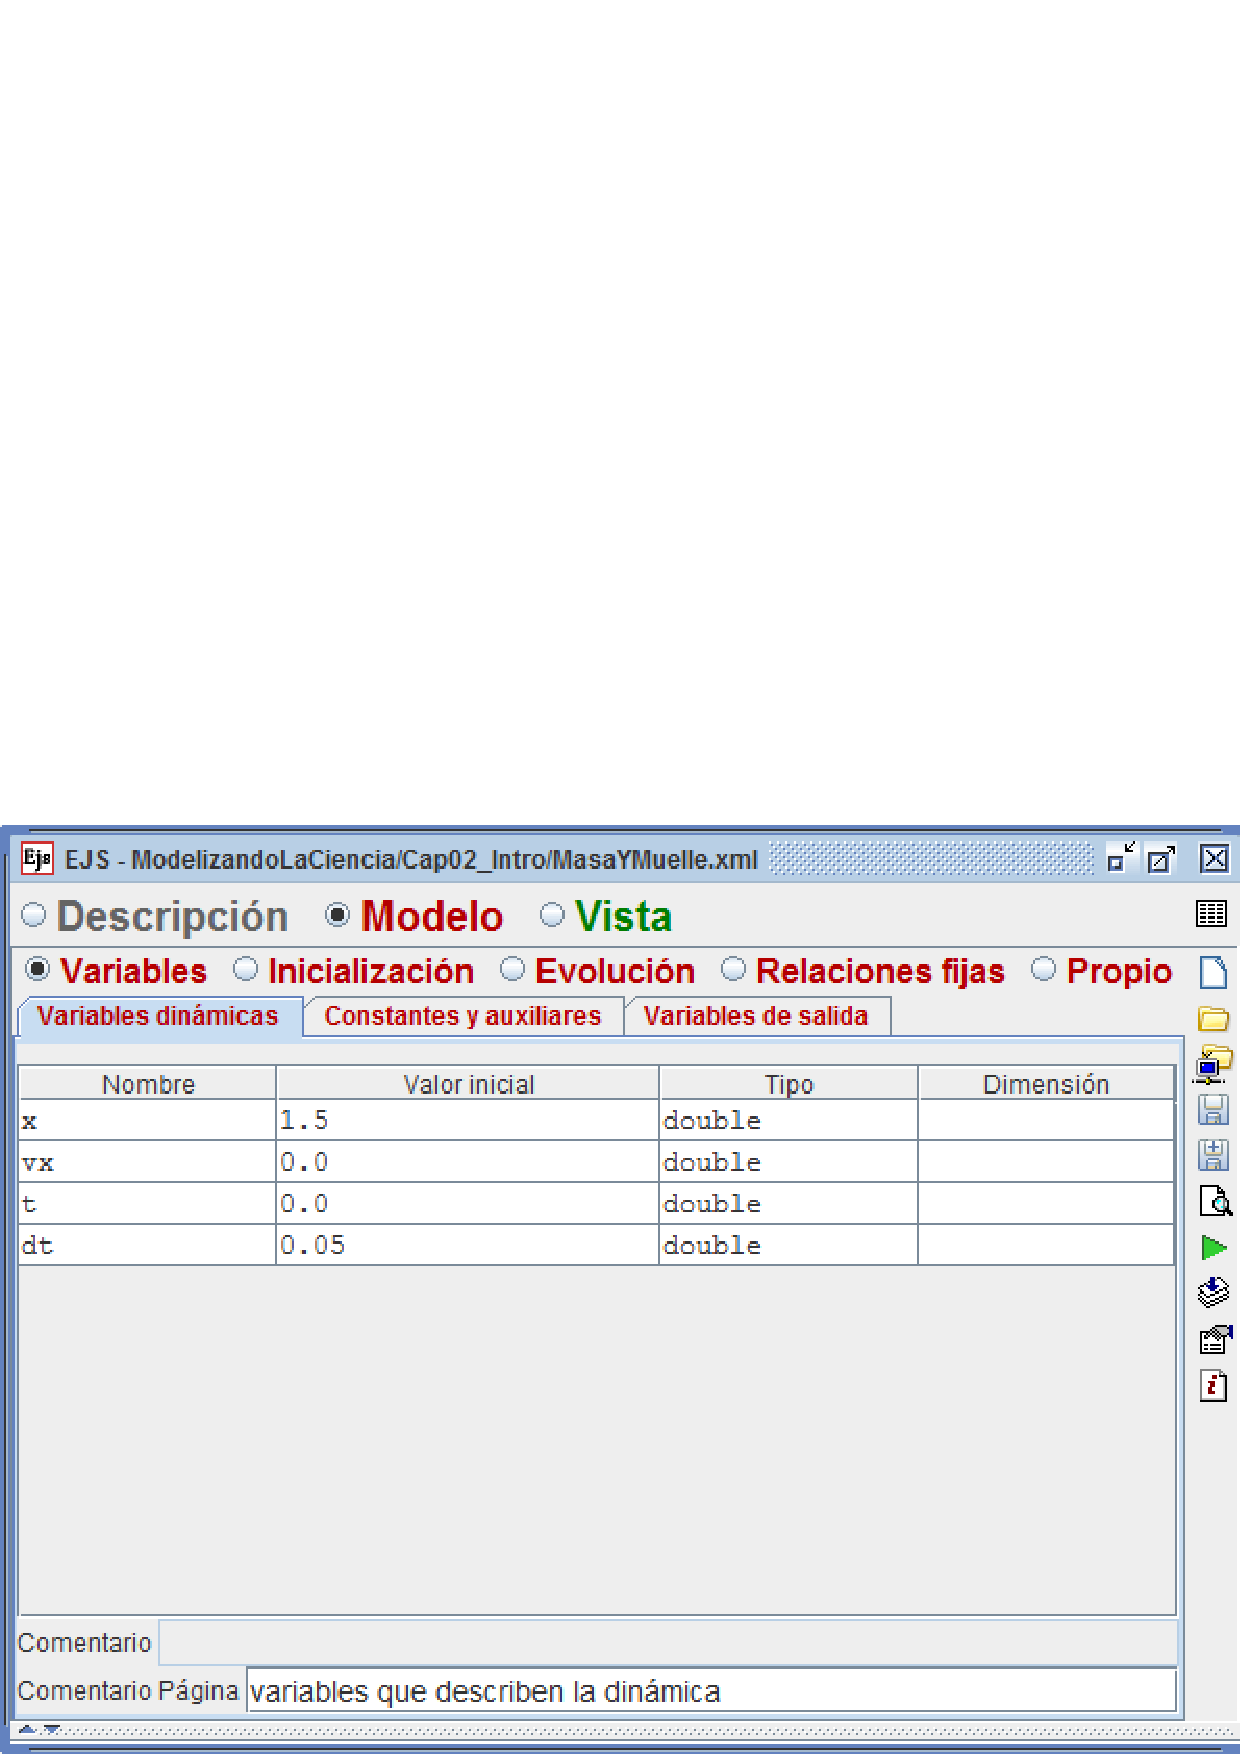
\includegraphics[scale=\scale]{02ExplorationJava/images/ModelVariables.png}
    \caption{The \lit{Model} workpanel contains six subpanels. The subpanel for the definition of mass and spring dynamical variables is displayed.  Other tabs in this subpanel define additional variables, such as the natural length of the spring $L$ and the energy $E$.} \label{fig:02ExplorationJava/ModelVariables}
\end{figure}

When implementing a model, a good first step is to identify, define, and initialize the variables that describe the
system. The term \emph{variable} is very general and refers to anything that can be given a name, including a
physical constant and a graph\index{Model!Variables}. Figure~\ref{fig:02ExplorationJava/ModelVariables} shows an
\ejs\ variable table. Each row defines a variable of the model by specifying the name of the variable, its type, its dimension, and its initial value.

Variables in computer programs can be of several types depending on the data they hold. The most frequently used types are \code{boolean} for true/false values, \code{int} for integers, \code{double} for high-precision ($\approx 16$ significant digits) numbers, and \code{String} for text.  We will use all these variable types in this document, but the mass and spring model uses only variables of type \code{double} and \code{boolean}.

Variables can be used as parameters, \index{Model!Parameters} state variables,\index{Model!State variables} or inputs and outputs of the model.\index{Model!Input and Output}  The tables in Figure~\ref{fig:02ExplorationJava/ModelVariables} define the variables used within our model.  We have
declared a variable for the $x$-position of the particle, \code{x}, for its velocity in the
$x$-direction, \code{vx}, for the time, \code{t}, and for the increment of time at each simulation step, \code{dt}.
We define some variables, in this and other tabs, that do not appear in Equation\eqref{eq:02ExplorationJava/SpringBasic}. The reason for auxiliary variables, such as  \code{vx} or the kinetic, potential, and total energies, will be made clear in what follows. The bottom part of the variables panel contains a comment field that provide a description of the role of each variable in the model. Clicking on a variable displays the corresponding comment.

\subsubsection{Initialization of the model}
Correctly setting initial conditions is important when implementing a model because the model must start in a
physically realizable state. Our model is relatively simple, and we initialize it by entering values (or simple Java
expressions such as \code{0.5*m*vx*vx}) in the \lit{Initial value} column of the table of variables. \ejs\ uses these values when it initializes the simulation.

\note{Advanced models may require an initialization algorithm. For example, a molecular dynamics model may set particle
velocities for an ensemble of particles. The \lit{Initialization} panel allows us to define one or more pages of Java
code that perform the required computation. \ejs\ converts this code into a Java method\index{Java!method}\footnote{A
Java method is similar to a function or a subroutine in procedural computer languages.} and calls this method at
start-up and whenever the simulation is reset. The mass and spring \lit{Initialization} panel is not shown here because
it is empty. See Subsection~\ref{section:02ExplorationJavaInspectingRelations} for an example of how Java code appears in \ejs.}

\subsubsection{The evolution of the model}

The \lit{Evolution} panel allows us to write the Java code that determines how the mass and spring system evolves in time and we will use this option frequently for models not based on ordinary differential equations (ODEs). There is, however, a second option that allows us to enter ordinary differential equations, such as \eqref{eq:02ExplorationJava/SpringBasic}, without programming.  \ejs\ provides a dedicated editor that lets us specify differential equations in a format that resembles mathematical
notation and automatically generates the correct Java code.

Let's see how the differential equation editor works for the mass and spring model. Because ODE algorithms solve
systems of first-order ordinary differential equations, a higher-order equation, such as
\eqref{eq:02ExplorationJava/SpringBasic}, must be recast into a first-order system.   We can do so by treating the
velocity as an independent variable which obeys its own equation:
\begin{align}
  \frac{d\ x} {dt} &= v_x                           \label{eq:02ExplorationJava/SpringBasicODE1} \\
  \frac{d\ v_x}{dt} &= -\frac{k}{m}\,(x-L). \label{eq:02ExplorationJava/SpringBasicODE2}
\end{align}
The need for an additional differential equation explains why we declared the \code{vx} variable in our table of
variables.

Clicking on the \lit{Evolution} panel displays the ODE editor shown in
Figure~\ref{fig:02ExplorationJava/ModelEvolution}.
\begin{figure}[htb]
    \centering
  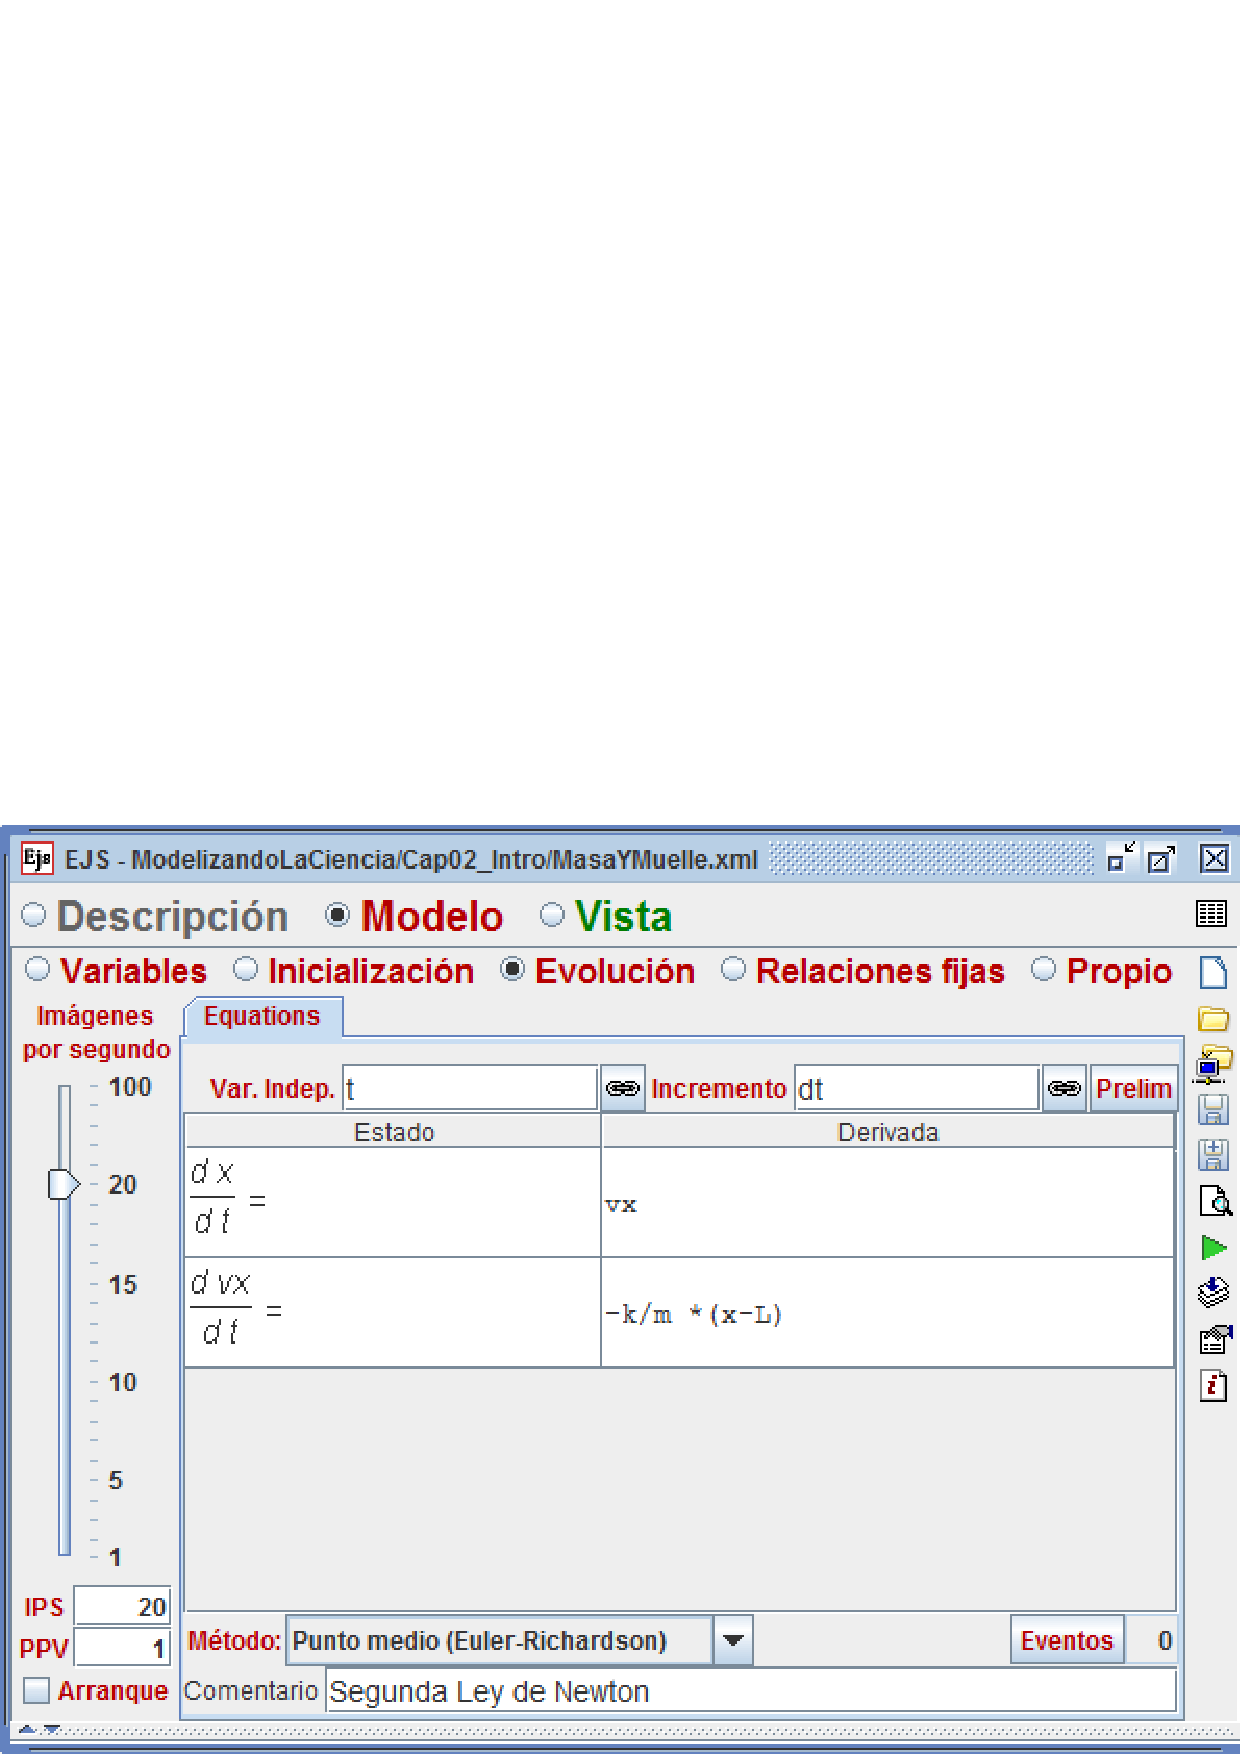
\includegraphics[scale=\scale]{02ExplorationJava/images/ModelEvolution.png}
    \caption{The ODE evolution panel showing the mass and spring differential equation and the numerical algorithm.}
    \label{fig:02ExplorationJava/ModelEvolution}
\end{figure}
Notice that the ODE editor displays \eqref{eq:02ExplorationJava/SpringBasicODE1} and \eqref{eq:02ExplorationJava/SpringBasicODE2}
(using the  \lit{*} character to denote multiplication). Fields near the top of the editor specify the independent variable
\code{t} and the variable increment \code{dt}.  Numerical algorithms approximate the exact ODE solution by advancing
the state in discrete steps and the increment determines this step size.
The \lit{Prelim code} button at the top-right of the editor allows us to enter preliminary code, to perform computations prior to evaluating the equations (a circumstance required in more complex situations than the one we treat in this example). A dropdown menu at the bottom of the editor
lets us select the ODE solver (numerical algorithm) that advances the solution from the current value of time, \code{t}, to the next value, \code{t + dt}. The tolerance field (\lit{Tol}) is greyed out and empty because Euler--Richardson is a fixed-step method that requires no tolerance settings. The advanced button displays a dialog which allows us to fine-tune the execution of this solver, though default values are usually appropriated. Finally, the events field at the bottom of the panel tells us that we have not defined any events for this differential equation. Examples with preliminary code and events can be found further on in this document. The different solver algorithms and its parameters are discussed in the \ejs\ help.

The left-hand side of the evolution workpanel includes fields that determine how smoothly and how fast the simulation runs.
The \lit{frames per second} (\lit{FPS}) option, which can be selected by using either a slider or an input field,
specifies how many times per second we want our simulation to repaint the screen. The \lit{steps per display}
(\lit{SPD}) input field specifies how many times we want to advance (step) the model before repainting. The current
value of \code{20} frames per second produces a smooth animation that, together with the prescribed value of one step
per display and \code{0.05} for \code{dt}, results in a simulation which runs  at (approximately) real time. We will
almost always use the default setting of one step per display. However, there are situations where the model's
graphical output consumes a significant amount of processing power and where we want to speed the numerical
computations. In this case we can increase the value of the steps per display parameter so that the model is advanced
multiple times before the visualization is redrawn. The \lit{Autoplay} check box indicates whether the simulation
should start when the program begins. This box is unchecked so that we can change the initial conditions before
starting the evolution.

The evolution workpanel handles the technical aspects of the mass and spring ODE model without programming.  The
simulation advances the state of the system by numerically solving the model's differential equations using the
midpoint algorithm. The algorithm steps from the current state at time \code{t} to a new state at a new time
\code{t + dt} before the visualization is redrawn. The simulation repeats this evolution step \code{20} times per second
on computers with modest processing power. The simulation may run slower and not as smoothly on computers with
insufficient processing power or if the computer is otherwise engaged, but it should not fail.

\note{Although the mass and spring model can be solved with a simple ODE algorithm, our numerical methods library
contains very sophisticated algorithms and \ejs\ can apply these algorithms to large systems of vector differential
equations with or without discontinuous events.}

\subsubsection{Relations among variables}\label{section:02ExplorationJavaInspectingRelations}
Not all variables within a model are computed using an algorithm on the Evolution workpanel. Variables can also be computed after the evolution has been applied. We refer to variables that are computed using the evolution algorithm as state variables or dynamical variables, and we refer to variables that depend on these variables as auxiliary or output variables. In the mass and
spring model the kinetic, potential, and total energies of the system are output variables because they are computed
from state variables.
\begin{align}
  T &= \frac{1}{2} m {v_x}^2,     \label{eq:02ExplorationJava/SpringEnergy1} \\
  V &= \frac{1}{2} k (x-L)^2,     \label{eq:02ExplorationJava/SpringEnergy2} \\
  E &= T + V.                     \label{eq:02ExplorationJava/SpringEnergy3}
\end{align}
We  say that there exists \emph{fixed relations} among the model's variables.

The \lit{Fixed relations} panel shown in Figure~\ref{fig:02ExplorationJava/ModelRelations} is used to write relations among
variables. Notice how easy it is to convert \eqref{eq:02ExplorationJava/SpringEnergy1} through
\eqref{eq:02ExplorationJava/SpringEnergy3} into Java syntax. Be sure to
use the multiplication character \lit{*} and to place a semicolon at the end of each Java statement.

\begin{figure}[htb]
    \centering
  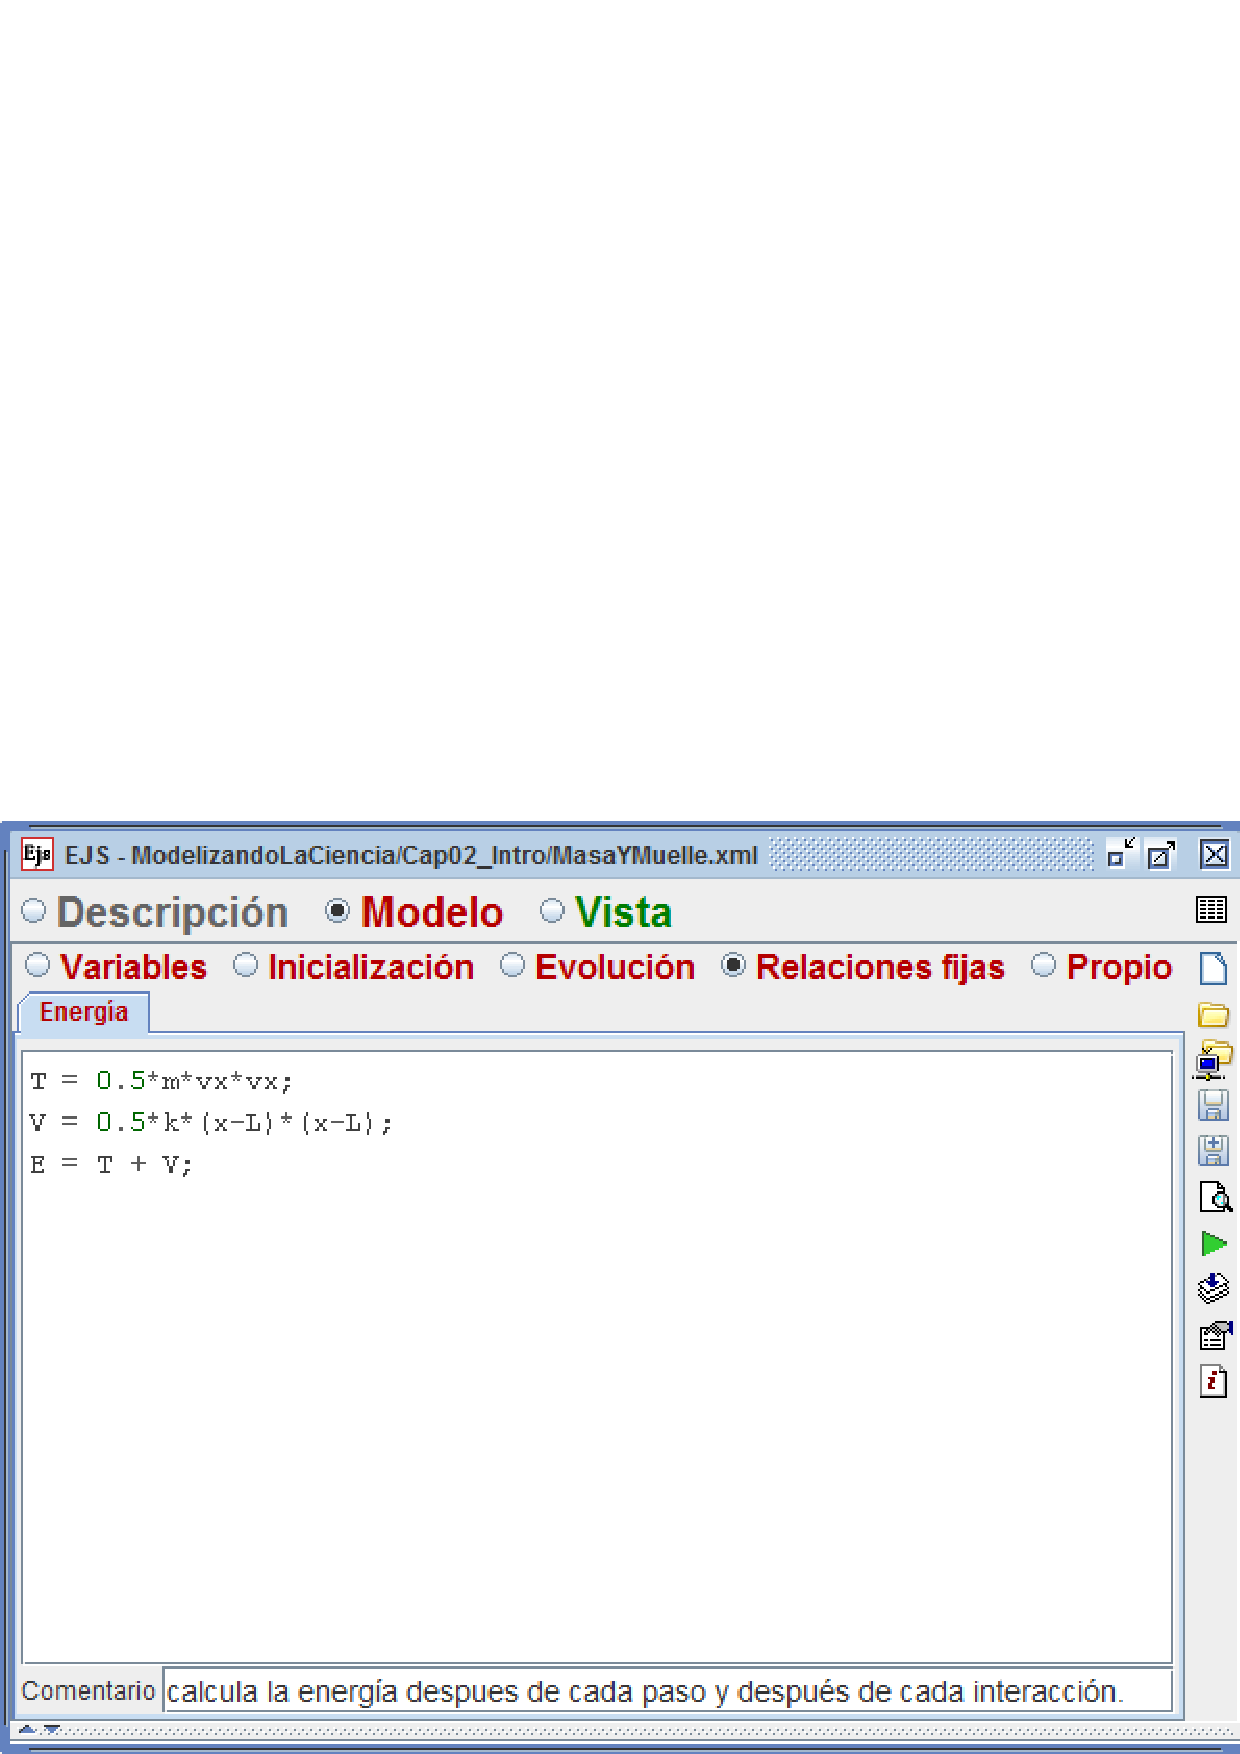
\includegraphics[scale=\scale]{02ExplorationJava/images/ModelConstraints.png}
    \caption{Fixed relations for the mass and spring model.}
    \label{fig:02ExplorationJava/ModelRelations}
\end{figure}

\noindent \textbf{Here goes an important remark.} You may wonder why we do not write fixed relation expressions by adding a second code page after the ODE page in the
\lit{Evolution} panel. After all, evolution pages execute sequentially and a second evolution page would correctly
update the output variables after every step. The reason that the \lit{Evolution} panel should not be used is that
relations must \emph{always} hold and there are other ways, such as mouse actions, to affect state
variables. For example, dragging the mass changes the $x$ variable and this change affects the energy.
\ejs\ automatically evaluates the relations after initialization, after every evolution step, and whenever
there is any user interaction with the simulation's interface.  For this reason, it is important that fixed relations among variables be written in the \lit{Fixed relations} workpanel.

\subsubsection{Custom pages}

There is a fifth panel in the \lit{Model} workpanel labeled \lit{Custom}. This panel can be used to define Java methods (functions) that can be used throughout the model.  This panel is empty because our model currently doesn't require additional methods,
but we will make use of this panel when we modify our mass and spring example in Section~\ref{section:02ExplorationJavaModifying}.  A
custom method is not used unless it is explicitly invoked from another workpanel.

\subsubsection{Model elements}

The final, sixth panel in the \lit{Model} workpanel is labeled \lit{Elements} and provides access to third-party Java libraries in the form of drag and drop icons. You add these libraries to your program by dragging the corresponding icon to the list of model elements to use for this model. This creates Java objects you can then use in your model code. This panel is also empty for this model because our mass and spring doesn't require additional Java libraries.

% ---------------------------------------------
\subsection{The \lit{View} workpanel}
% ---------------------------------------------

The third \Ejs\ workpanel is the \lit{View}.  This workpanel allows us to create a graphical interface that includes
visualization, user interaction, and program control with minimum programming.
Figure~\ref{fig:02ExplorationJava/SpringInterface} shows the view for the mass and spring model. Select the \lit{View} radio
button to examine how this view is created.

The right frame of the view workpanel of \ejs, shown in Figure~\ref{fig:02ExplorationJava/View}, contains a collection of
\emph{view elements},\index{Ejs!view elements} grouped by functionality. View elements are building blocks that can be
combined to form a complete user interface, and each view element is a specialized object with an on-screen
representation. To display information about a given element, click on its icon and press the \lit{F1} key or right-click and select the \lit{Help} menu item. To create a user interface, we create a frame (window) and add elements, such as buttons and graphs, using ``drag and drop'' as described in Section~\ref{section:02ExplorationJavaModifying}.

\begin{figure}[htb]
    \centering
  \includegraphics[scale=\scale]{02ExplorationJava/images/View.png}
    \caption{The \lit{View} workpanel showing the \emph{Tree of elements} for the mass and spring user interface.}
    \label{fig:02ExplorationJava/View}
\end{figure}

The \emph{Tree of elements} shown on the left side of Figure~\ref{fig:02ExplorationJava/View} displays the structure of the
mass and spring user interface. Notice that the simulation has two windows, a \code{Frame} and a \code{Dialog}, that appear on your computer screen.
These elements belong to the class of \emph{container} elements whose primary
purpose is to visually group (organize) other elements within the user interface.
The tree displays descriptive names and icons for these elements.   Right-click on an element of the tree to
obtain a menu that helps the user change this structure. Alternatively, you can drag and drop elements from one container to another to change the parent-child relationship, or within a container to change the child order. (There are conditions for a container to accept a given element as child. For instance, a two-dimensional drawing panel can only accept 2D drawable elements.)

Each view element has a set of internal parameters, called \emph{properties},\index{Ejs!view element properties} which
configure the element's appearance and behavior. We can edit these properties by double clicking on the element in the
tree to display a table known as a \emph{properties inspector}.  Appearance properties, such as color, are often set to a constant value, such as \code{RED}. We can also use a variable from the model to set an element's property. This ability to connect (bind) a property to a variable without programming is the key to turning our view into a dynamic and interactive
visualization.

Let's see how this procedure works in practice. Double-click on the \code{massShape2D} element (the `Shape2D' suffix we added to the element's name helps you know the type of the element) in the tree to display
the element's properties inspector. This element is the mass that is attached at the free end of the spring. The massShape2D's table of properties appears as shown in Figure~\ref{fig:02ExplorationJava/SpringBallProperties}.
\begin{figure}[htb]
    \centering
  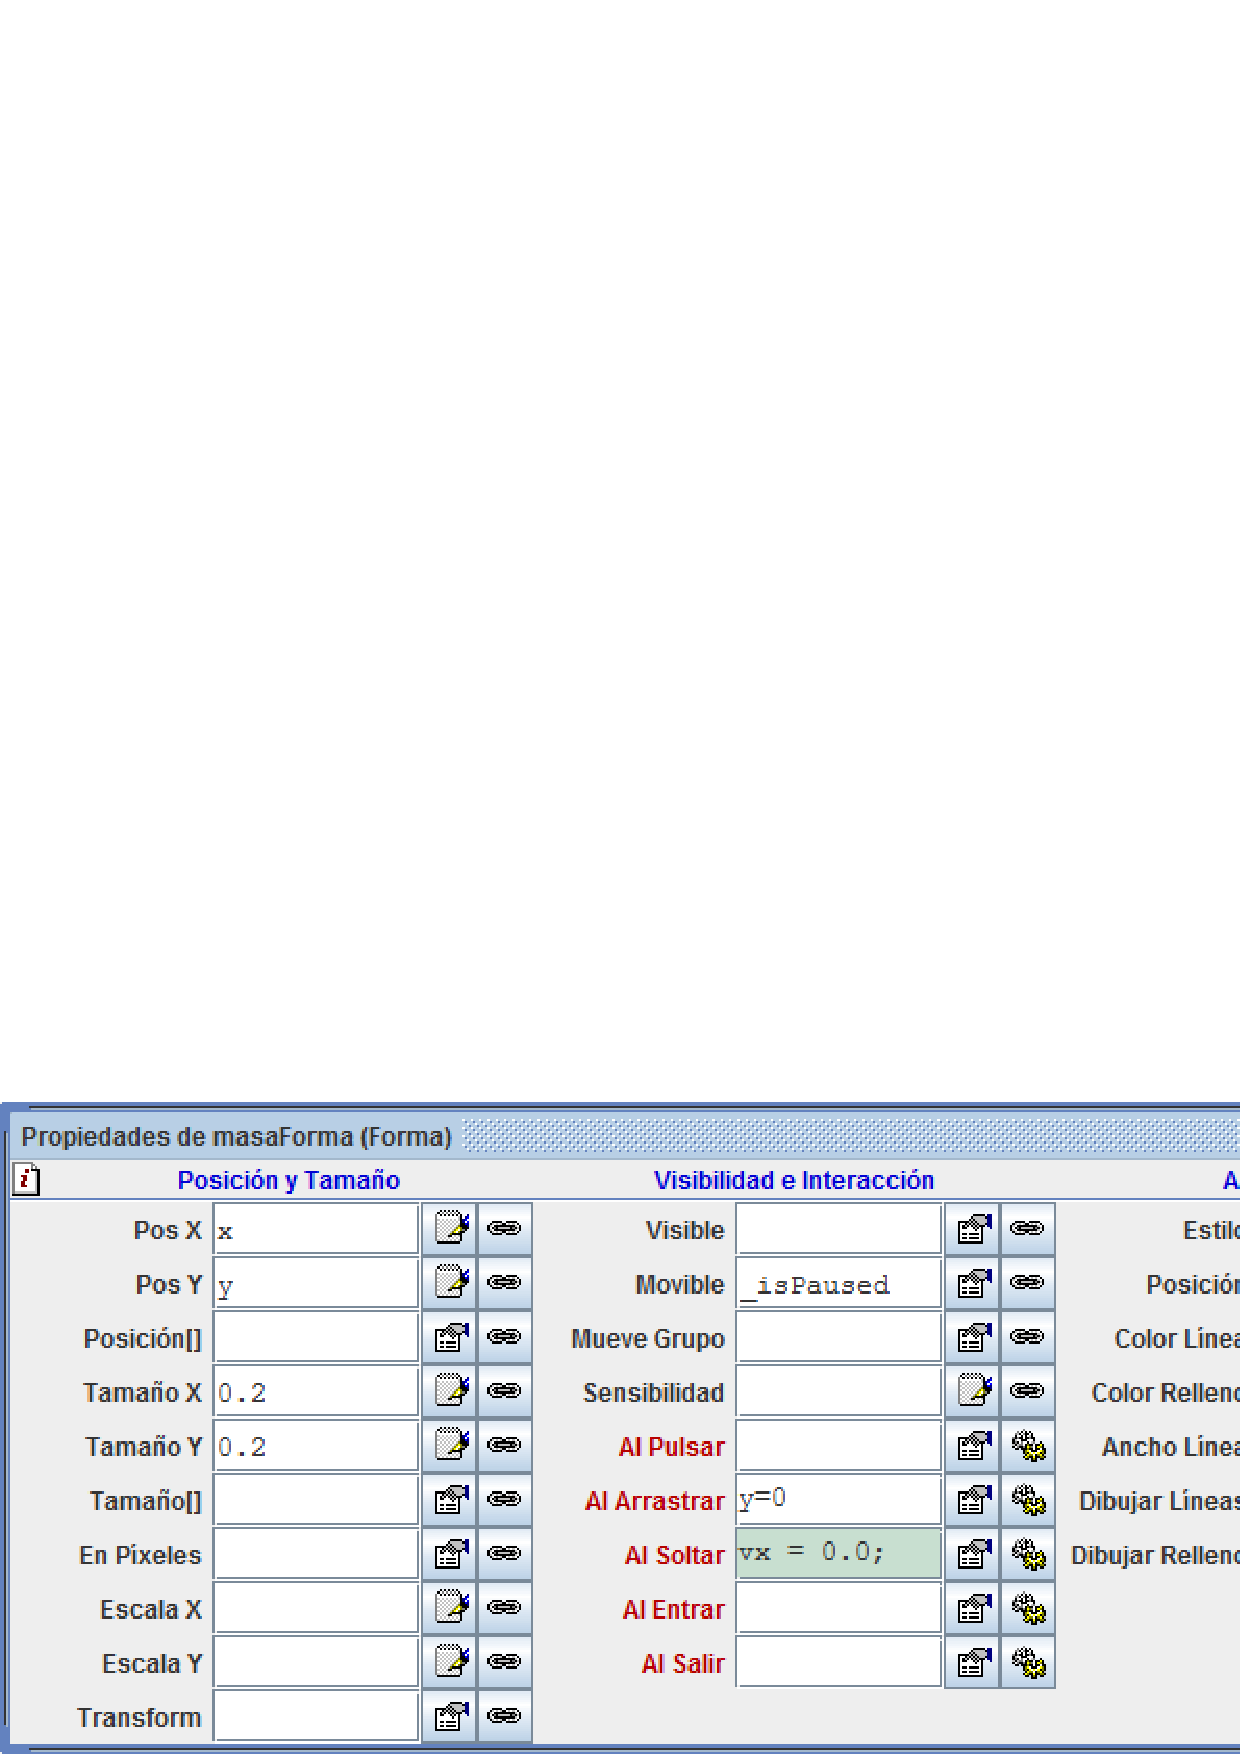
\includegraphics[scale=\scale]{02ExplorationJava/images/SpringBallProperties.png}
    \caption{The table of properties of the \code{massShape2D} element.}
    \label{fig:02ExplorationJava/SpringBallProperties}
\end{figure}

Notice the properties that are given constant values. The \code{Style}, \code{Size X}, \code{Size Y}, and \code{Fill
Color} properties produce an ellipse of size \code{(0.2,0.2)} units (which makes a circle) filled with the color
magenta. More importantly, the \code{Pos X} and \code{Pos Y} properties of  the shape are bound to the \code{x} and \code{y}
variables of the model. This simple assignment establishes a bidirectional connection between model and view. These
variables change as the model evolves and the shape follows the \code{x} and \code{y} values. If the user drags the
shape to a new location, the \code{x} and \code{y} variables in the model change accordingly.  Note that the \code{Draggable} property is only enabled when the animation is paused.

Elements can also have \emph{action properties}\index{Ejs!action properties} which can be associated with code.
(Action properties have their labels displayed in red.) User actions, such as dragging or clicking, invoke their
corresponding action property, thus providing a simple way to control the simulation. As the user drags the mass, the code on the \code{On Drag} property restricts the motion of the shape to the horizontal direction by setting the \code{y} variable to \code{0}.  Finally, when the mouse button is
released, the following code is executed:

\begin{listing}
\begin{verbatim}
vx = 0.0;            // sets the velocity to zero
_view.resetTraces(); // clears all plots
\end{verbatim}
\end{listing}

\noindent Clicking on the icon next to the field displays a small editor that shows this code.

\note{Because the \code{On Release} action code spans more than one line, the property field in the inspector shows a darker (green) background. Other data types, such as boolean properties, have different editors.  Clicking the second icon displays a dialog window with a listing of variables and methods that can be used to set the property value.}

\begin{exercise}[Element inspectors]\label{ex:02ExplorationJava/properties}
The mass' inspector displays different types of properties and their possible values. Explore the properties of other
elements of the view.  For instance, the \code{displacementTrail2D} and \code{velocityTrail2D} elements correspond to the
displacement and velocity time plots in the second window of the view, respectively.  What is the maximum number of points that can be added to each trail?
\end{exercise}

\subsection{The completed simulation}

We have seen that \Ejs\ is a powerful tool that lets us express our knowledge of a model at a very high level of abstraction. When modeling the mass and spring, we first created a table of variables that describes the model and initialized these variables using a column in the table. We then used an evolution panel with a high-level editor for systems of first-order ordinary differential equations to specify how the state advances in time. We then wrote relations to compute the auxiliary or output variables that can be expressed using expressions involving state variables.  Finally, the program's graphical user interface and high-level visualizations were created by dragging objects from the \lit{Elements} palette into the \lit{Tree of elements}. Element properties were set using a properties editor and some properties were associated with variables from the model.

It is important to note that the three lines of  code on the Fixed relations workpanel (Figure~\ref{fig:02ExplorationJava/ModelRelations}) and the two lines of code in the particle's action method are the only explicit Java code needed to implement the model.  \Ejs\ creates a complete Java program by processing the information in the workpanels when the run icon is pressed as described in Section~\ref{section:02ExplorationJavaRunning}.

% -----------------------------------------------------
\section{Running the Simulation}\label{section:02ExplorationJavaRunning}\index{Simulation!running}
% -----------------------------------------------------

It is time to run the simulation by clicking on the \lit{Run} icon of the taskbar, 
\includegraphics[scale=\linescale]{../_common/icons_png/launch.png}.  \ejs\ generates the Java code and compiles it, collects auxiliary and library files, and executes the compiled program. All at a single mouse click.

Running a simulation initializes its variables and executes the fixed relations to insure that the model is in a consistent state.  The model's time evolution starts when the play/pause button in the user interface is pressed. (The play/pause button displays the 
\includegraphics[scale=\linescale]{../_common/icons_png/play.png} icon when the simulation is paused and 
\includegraphics[scale=\linescale]{../_common/icons_png/pause.png} when it is running.) In our current example, the program executes a numerical method to advance the harmonic oscillator differential equation by $0.05$ time units and then executes the fixed relations code.  Data are then passed to the graph and the graph is repainted. This process is repeated $20$ times per second.

When running a simulation, \ejs\ changes its \lit{Run} triangle icon to a red \lit{Kill} square and prints informational messages saying that the
simulation has been successfully generated and that it is running. Notice that the two \ejs\ windows disappear and are
replaced by new but similar windows without the \code(Ejs window) suffix in their titles.  These views respond to user
actions. Click and drag the particle to a desired initial horizontal position and then click on the play/pause button.
The particle oscillates about is equilibrium point and the plot displays the displacement and velocity data as shown in
Figure~\ref{fig:02ExplorationJava/SpringRunning}.

Stop the simulation and right-click the mouse over any of the drawing areas of the simulation. In the popup menu that appears, select the \code{Elements options->plottingPanel->Data Tool} entry to display and analyze the data generated by the model.  The same popup menu offers other run-time options, such as screen capture.  To exit the program, close the simulation's main window.

\begin{figure}[htb]
  \centering
  \subfigure{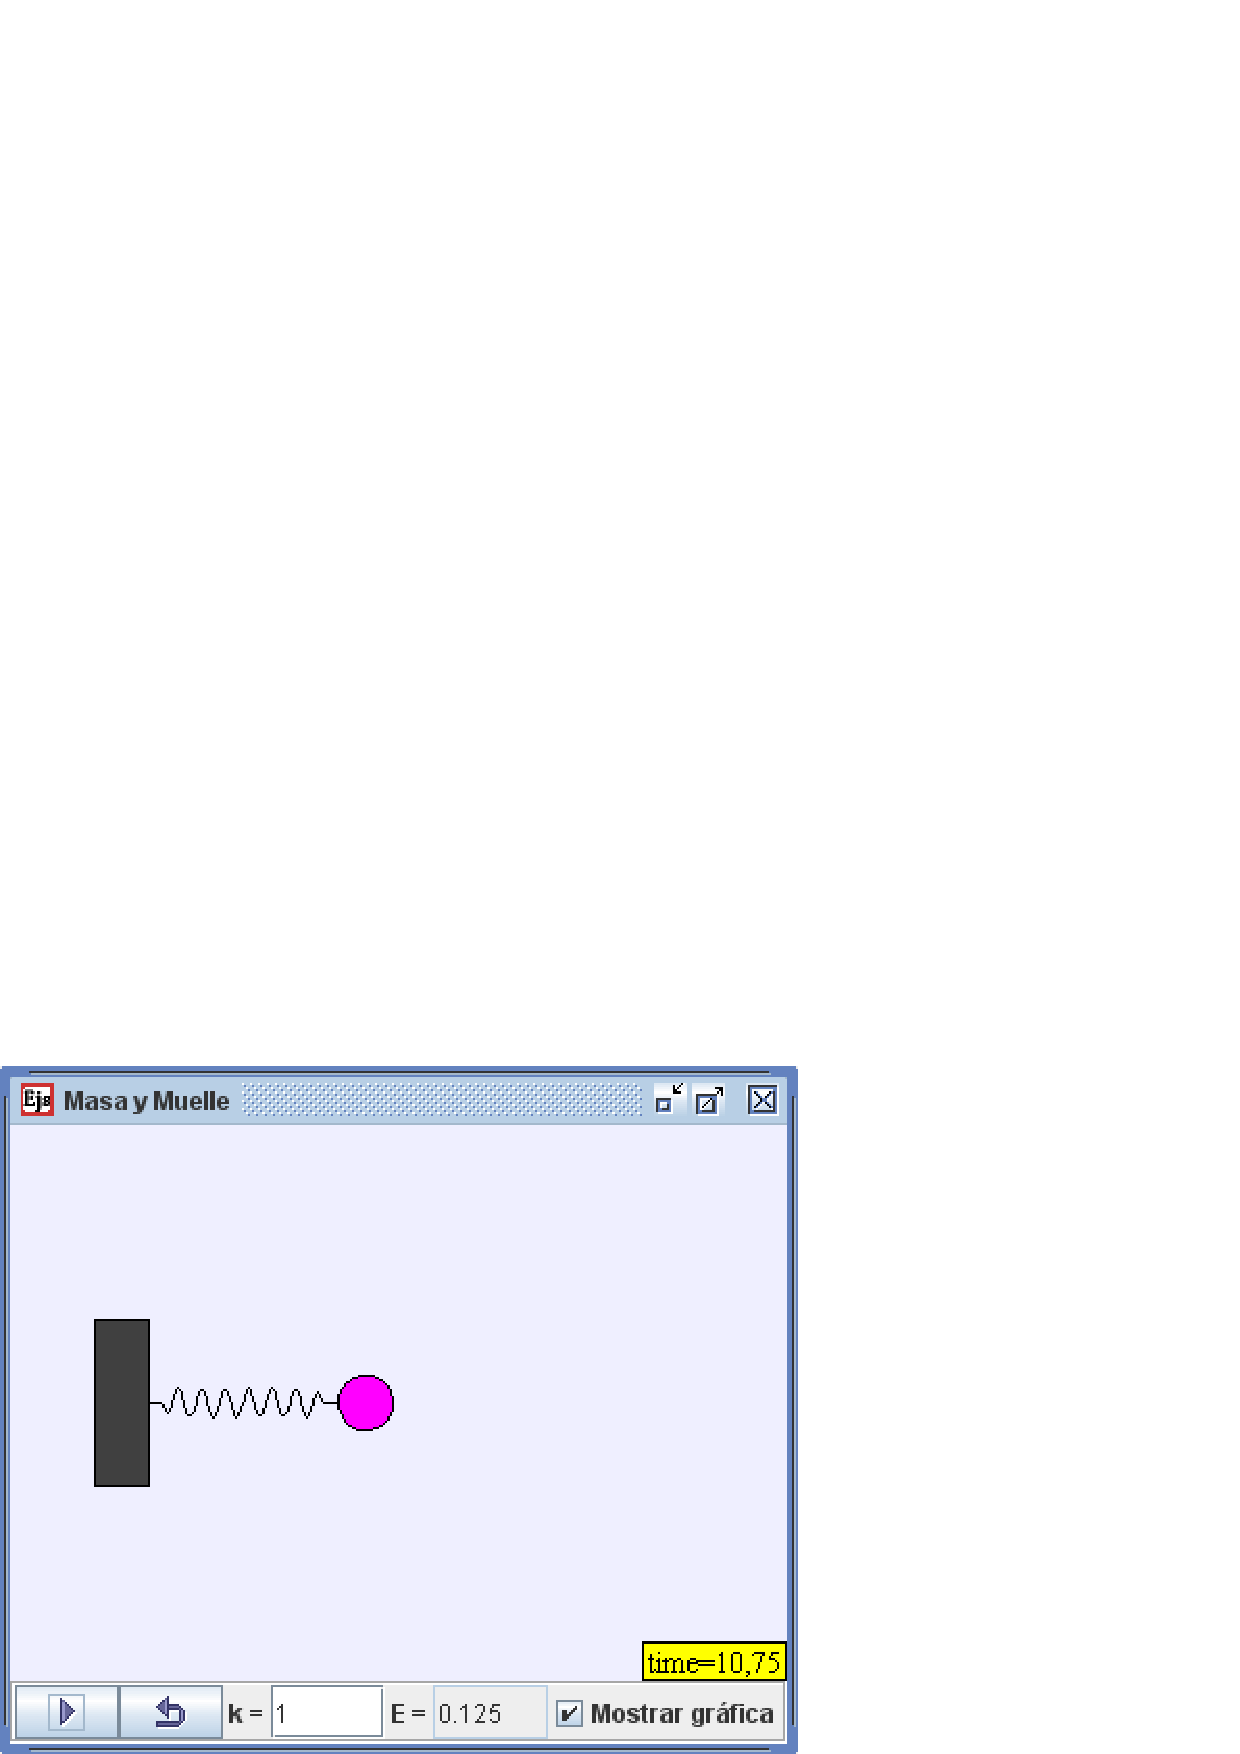
\includegraphics[scale=\scale]{02ExplorationJava/images/SpringRunning1.png}}
  \subfigure{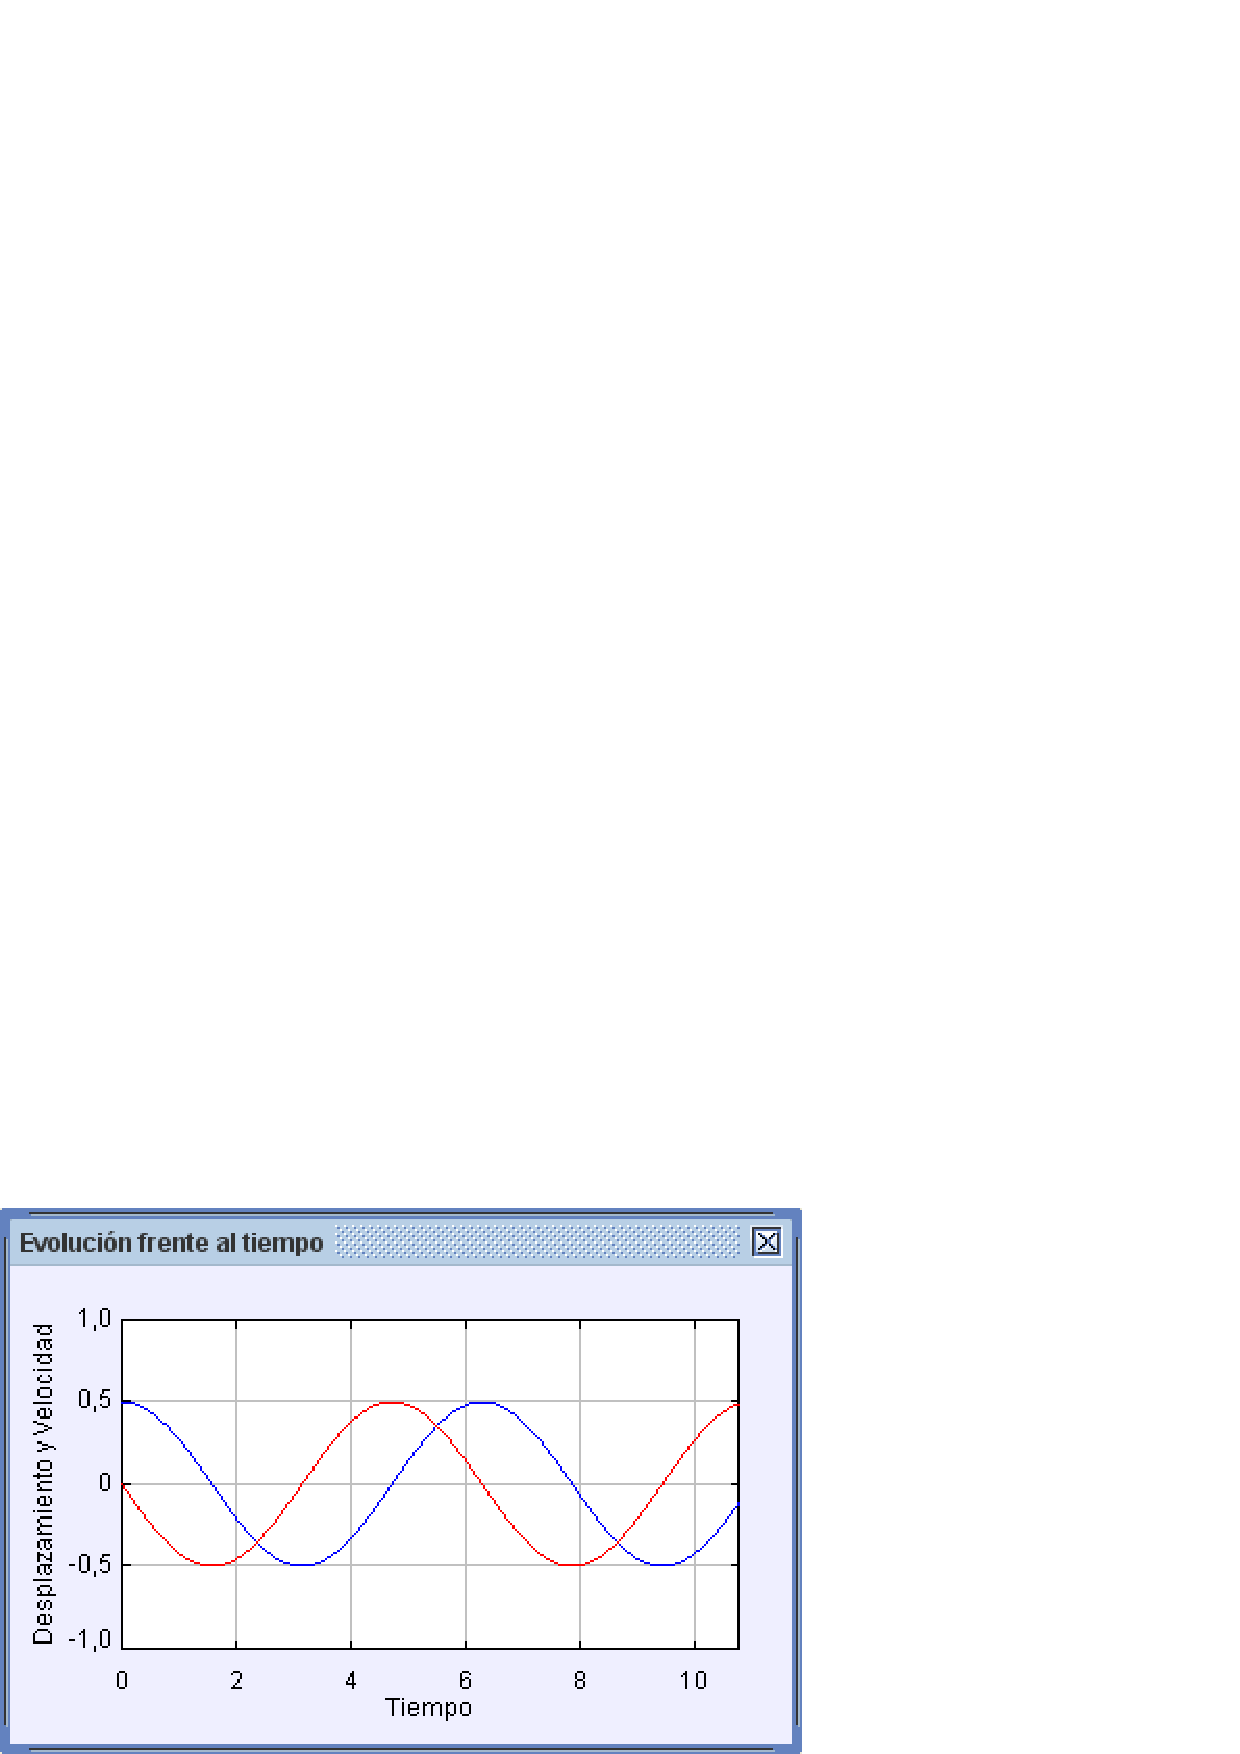
\includegraphics[scale=\scale]{02ExplorationJava/images/SpringRunning2.png}}
  \caption{The mass and spring simulation displays an interactive drawing of the model and a graph with displacement and velocity data.}
  \label{fig:02ExplorationJava/SpringRunning}
\end{figure}


% -----------------------------------------------------
\section{Distributing the Simulation}\label{section:02ExplorationJavaDistributing}\index{Simulation!distribution}
%
Simulations created with \ejs\ are stand-alone Java programs that can be distributed without \ejs\ for other people to use.  The easiest way to do this is to package the simulation in a single executable jar file by clicking on the \lit{Package} icon, 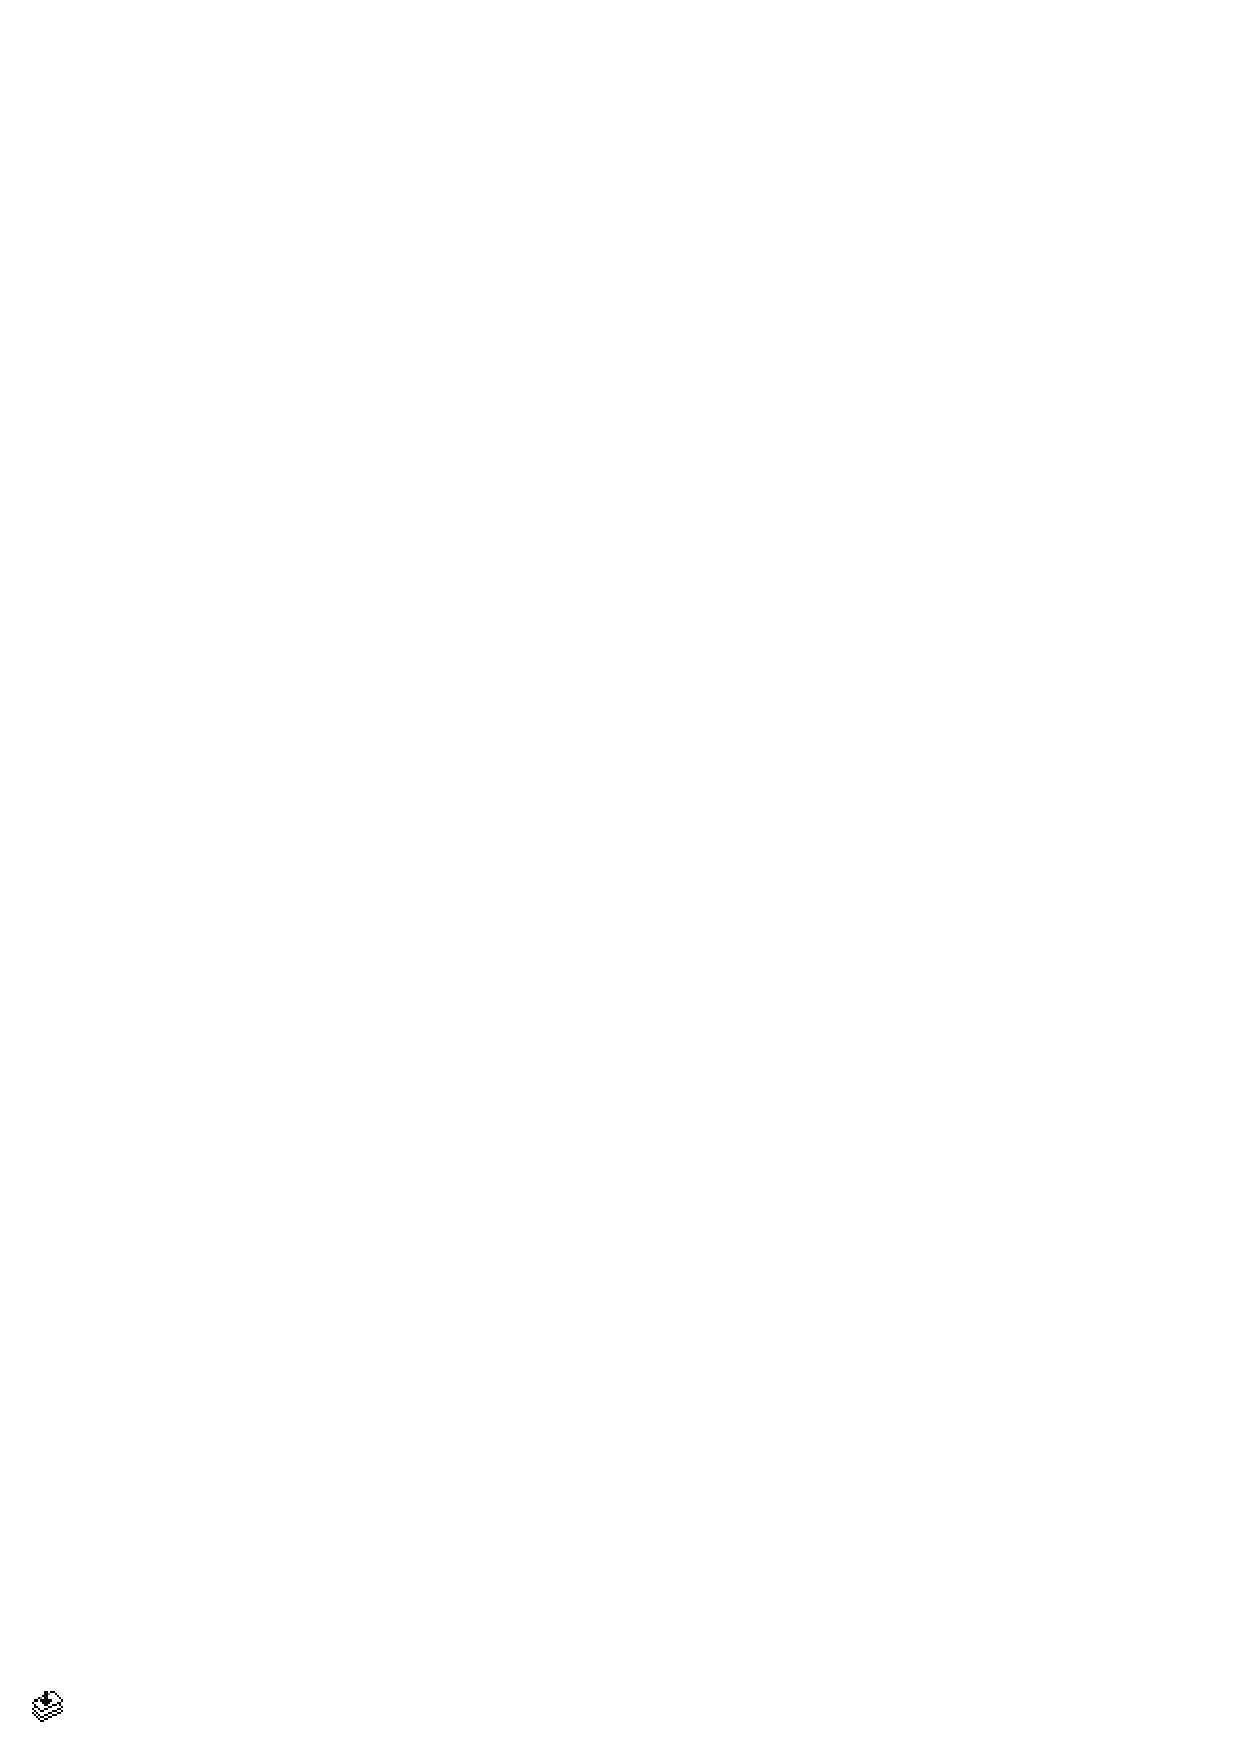
\includegraphics[scale=\linescale]{../_common/icons_png/package.png}. A file browser appears that lets you choose a name for the self-contained jar package.  The default target directory to hold this package file is the \file{export} directory of your workspace, but you can choose any directory and package name. The stand-alone jar file is ready to be distributed on a CD or via the Internet.  Other distribution mechanisms are available by right-clicking on the icon.
% as described in Appendix~\ref{appendix:Distribution}.

\begin{exercise}[Distribution of a model]\label{ex:02ExplorationJava/distribution}
Click on the \lit{Package} icon on the taskbar to create a stand alone jar archive of the mass and spring simulation.  Copy this jar file into a working directory separate from your \ejs\ installation.  Close \ejs\ and verify that the simulation runs as a stand-alone application.
\end{exercise}

Although the mass and spring jar file is a ready to use and to distribute Java application, an important pedagogic feature is that this jar file is created in such a way that users can return to \ejs\ at any time to examine, modify, and adapt the model. (\ejs\ must, of course, be installed.)  The jar file contains a small \emph{Extensible Markup Language} (XML) description of each model and right clicking on a drawing panel within the model brings in a popup menu with an option to copy this file into \ejs. This action will extract the required files from the jar, search for the \ejs\ installation in the user's hard disk, copy the files into the correct location, and run \ejs\ with this simulation loaded. If a model with the same name already exits, it can be replaced. The user can then inspect, run, and modify the model just as we are doing in this chapter.  A student can, for example, obtain an example or a template from an instructor and can later repackage the modified model into a new jar file for submission as a completed exercise.

\begin{exercise}[Extracting a model]\label{ex:02ExplorationJava/redistribution}
Run the stand-alone jar file containing the mass and spring model created in Exercise~\ref{ex:02ExplorationJava/distribution}.  Right click on the model's plot or drawing and select the \lit{Open Ejs Model} item from the popup menu to copy the packaged model back into \ejs.
\end{exercise}

\ejs\ is designed to be both a modeling and an authoring tool, and we suggest that you now experiment with it to learn
how you can create and distribute your own models. As a start, we recommend that you run the mass and spring simulation
and go through the activities in the second page of the \lit{Description} workpanel.  We modify this simulation in the next
section.

% -----------------------------------------------------
\section{Modifying the Simulation}\label{section:02ExplorationJavaModifying}
% -----------------------------------------------------

As we have seen, a prominent and distinctive feature of \Ejs\ is that it allows us to create and study a simulation at
a high level of abstraction. We inspected an existing mass and spring model and its user interface in the previous
section. We now illustrate additional capabilities of \Ejs\ by adding friction and a driving force and by adding a
visualization of the system's phase space.

\subsection{Extending the model}\label{section:02ExplorationJavaModifyingModel}
We can add damping in our model by introducing a viscous (Stoke's law) force that is proportional to the negative of
the velocity $F_f = - b\,v_x$ where $b$ is the damping coefficient. We also add an external time-dependent driving
force which takes the form of a sinusoidal function $F_e(t)=A\,\sin(\omega\, t)$. The introduction of these two forces
changes the second-order differential equation \eqref{eq:02ExplorationJava/SpringBasic} to
\begin{equation}
  \frac{d^2\ x}{dt^2} = -\frac{k}{m}\,(x-L) - \frac{b}{m}\,\frac{d\ x}{dt} + \frac{1}{m}\,F_e(t), \label{eq:02ExplorationJava/SpringComplete}
\end{equation}
or, as in equations \eqref{eq:02ExplorationJava/SpringBasicODE1} and \eqref{eq:02ExplorationJava/SpringBasicODE2}:
\begin{eqnarray}
  \frac{d\ x} {dt} &=& v_x,                  \label{eq:02ExplorationJava/SpringCompleteODE1} \\
  \frac{d\ v_x}{dt} &=& -\frac{k}{m}\,(x-L) - \frac{b}{m}\,v_x + \frac{1}{m}\,F_e(t). \label{eq:02ExplorationJava/SpringCompleteODE2}
\end{eqnarray}

\subsubsection{Adding variables}
The introduction of new force terms requires that we add variables for the coefficient of dynamic friction and for the amplitude and frequency of the sinusoidal driving force.  Return to the \lit{Model} workpanel of \ejs\ and select its \lit{Variables} panel. Right-click on the tab of the existing page of variables to see its popup menu, as in Figure~\ref{fig:02ExplorationJava/ModifyVariables1}.
Select the \lit{Add a new page} entry as shown in Figure~\ref{fig:02ExplorationJava/ModifyVariables1}. Enter \code{Damping and Driving Vars} for the new table name in the dialog and an empty table will appear.

\begin{figure}[htb]
    \centering
  \includegraphics[scale=\scale]{02ExplorationJava/images/ModifyVariables1.png}
    \caption{The popup menu for a page of variables.}
    \label{fig:02ExplorationJava/ModifyVariables1}
\end{figure}

We now use the new table to declare the needed variables. We could have used the already existing tables, but declaring multiple pages helps us organize the variables by category. Double-click on a table cell to make it editable and navigate through the table using the arrows or tab keys. Type \code{b} in the \lit{Name} cell of the first row, and enter the value \code{0.1} in the \lit{Initial value} cell to its right. We don't need to do anything else because the \code{double} type selected is already correct.
\ejs\ checks the syntax of the value entered and evaluates it. If we enter a wrong value, the background of the value cell will display a pink background.
Notice that when you fill in a variable name, a new row appears automatically. Proceed similarly to declare a new variable for the driving force's \code{amp} with value \code{0.2} and for its \code{freq} with value \code{2.0}. Document the meaning of these variables by typing a short comment for each at the bottom of the table. Our final table of variables is shown in Figure~\ref{fig:02ExplorationJava/ModifyVariables2}.  You can ignore the empty row at the end of the table or remove it by right-clicking on that row and selecting \lit{Delete} from the popup menu that appears.

\begin{figure}[htb]
    \centering
  \includegraphics[scale=\scale]{02ExplorationJava/images/ModifyVariables2.png}
    \caption{The new table of variables for the damping and forcing terms.}
    \label{fig:02ExplorationJava/ModifyVariables2}
\end{figure}

\subsubsection{Modifying the evolution}

We now modify the differential equations on the evolution page by adding expressions for the new terms in equation
\eqref{eq:02ExplorationJava/SpringCompleteODE2}. Go to the evolution panel, double-click on the \lit{Rate} cell of the
second equation, and edit it to read:

\begin{listing}
\begin{verbatim}
-k/m * (x-L) - b*vx/m + force(t)/m
\end{verbatim}
\end{listing}
Notice that we are using a method (function) named \code{force} that has not yet been defined.
We could have written an explicit expression for the sinusoidal function. However, defining a \code{force} method promotes cleaner and more readable code and allows us to introduce custom methods.

\subsubsection{Adding custom code}

The \code{force} method is defined using the \lit{Custom} panel of the \lit{Model}. Go to this panel and click on the
empty central area to create a new page of custom code. Name this page \lit{force}. You will notice that the
page is created with a code template that defines the method. Edit this code to read:

\begin{listing}
\begin{verbatim}
public double force (double time) {
  return amp*Math.sin(freq*time); // sinusoidal driving force
}
\end{verbatim}
\end{listing}
Type this code exactly as shown including capitalization. Compilers complain if there is any syntax error.

Notice that we pass the time at which we want to compute the driving force to the \texttt{force} method as an input parameter. Passing
the time value is very important. It would be incorrect to ask the method to use the value of the variable \code{t}, as
in:

\begin{listing}
\begin{verbatim}
public double force () { // incorrect implementation of the force method
  return amp*Math.sin(freq*t);
}
\end{verbatim}
\end{listing}

\noindent The reason that time must be passed to the method is that time changes throughout the evolution step.  In order for the ODE solver to correctly compute the time-dependent force throughout the evolution step, the time must be passed into the method that computes the rate.

\note{ Variables that change (evolve) must be passed to methods that are used to compute the rate because numerical solvers evaluate the \lit{Rate} column in the ODE workpanel at intermediate values between $t$ and $t+dt$. In other words, the independent variable and any other dynamic variable which is differentiated in the \lit{State} column of the ODE editor must be passed to any method that is called in the \lit{Rate} column. Variables which remain constant during an evolution step may be used without being passed as input parameters because the value of the variable at the beginning of the evolution step can be used.}

\subsection{Improving the view}\label{section:02ExplorationJavaModifyingView}
We now add a visualization of the phase space (displacement versus velocity) of the system's evolution to the
\lit{View}. We also add new input fields to display and modify the value of the damping, amplitude, and frequency parameters.

Go to the \lit{View} workpanel and notice that the \lit{Interface} palette contains many subpanels.  Click on the tab
with the 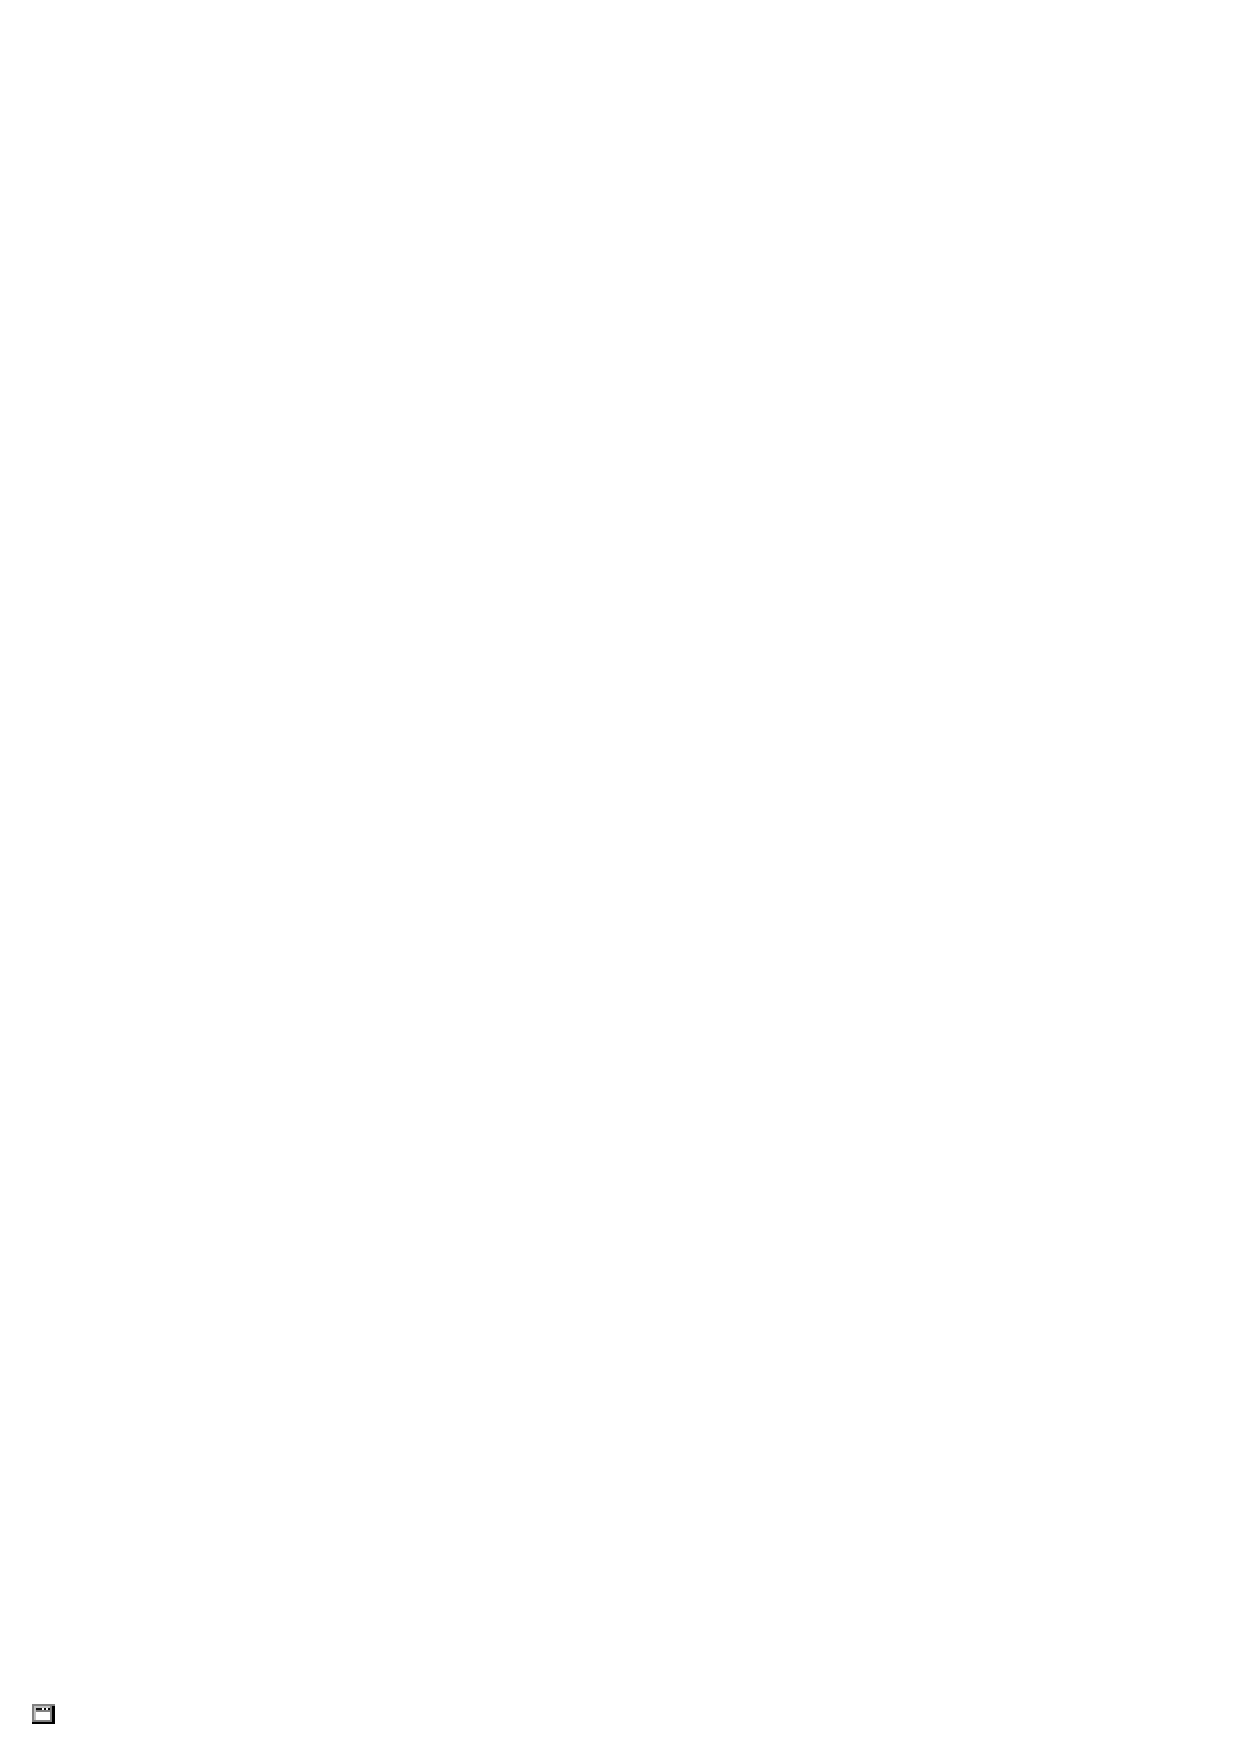
\includegraphics[scale=\linescale]{../_common/icons_png/Groups/Containers.png} icon to display the \lit{Windows, containers,
and drawing panels} palette of view elements.  Click on the icon for a plotting panel,
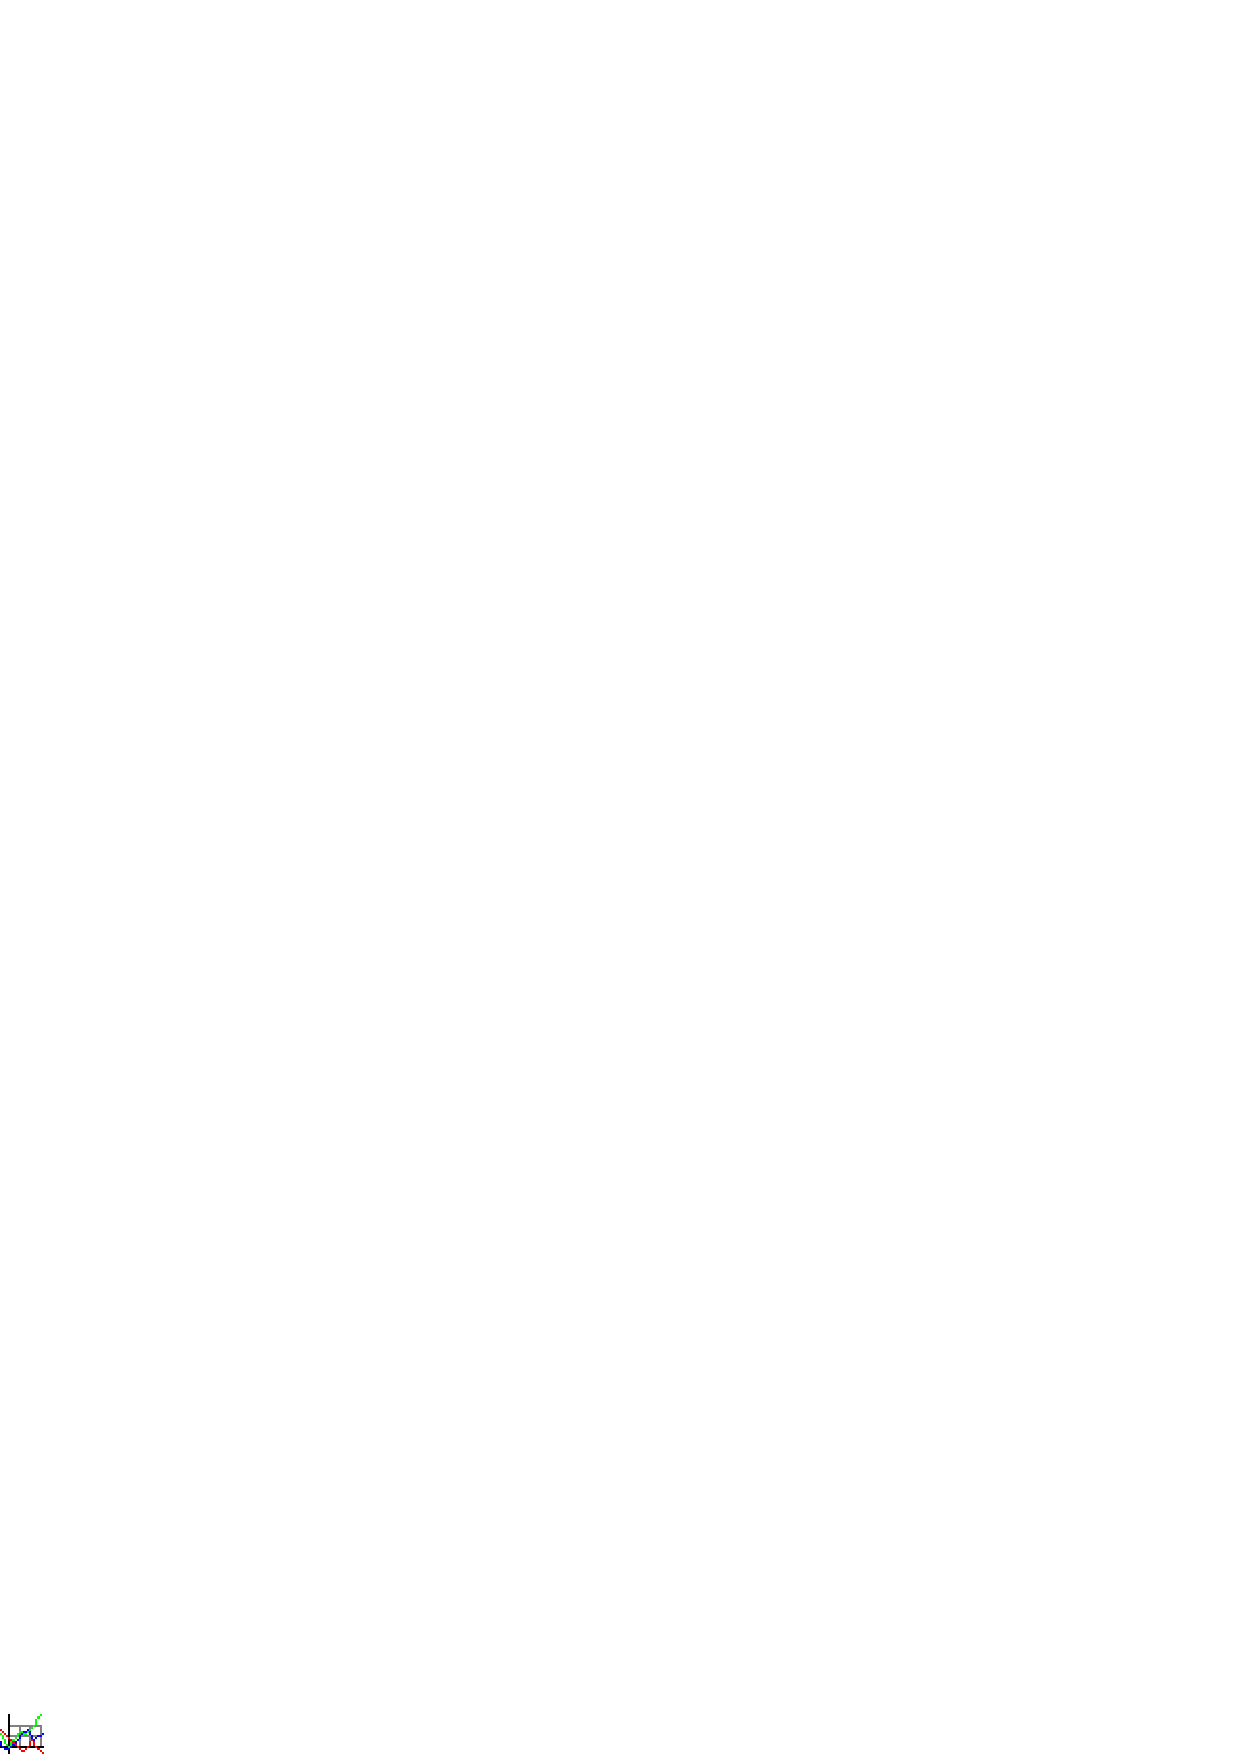
\includegraphics[scale=\linescale]{../_common/icons_png/Elements/PlottingPanel.png}, in this palette. You can rest (hover) the mouse
cursor over an icon to display a hint that describes the element if you have difficulty recognizing the icon.
Selecting an element sets a colored border around its icon on the palette and changes the cursor to a magic wand,

\includegraphics[scale=\linescale]{../_common/icons_png/create.png}. These changes indicate that \ejs\ is ready to create
an element of the selected type. (Return to the design mode --get rid of the magic wand-- by clicking on any
blank area within the \lit{Tree of elements} or hitting the \lit{Esc} key.)

Click on the \code{dialog} element in the \lit{Tree of elements} as shown in
Figure~\ref{fig:02ExplorationJava/ModifyViewAddPlottingPanel} to add the plotting panel to the view.

\begin{figure}[htb]
    \centering
  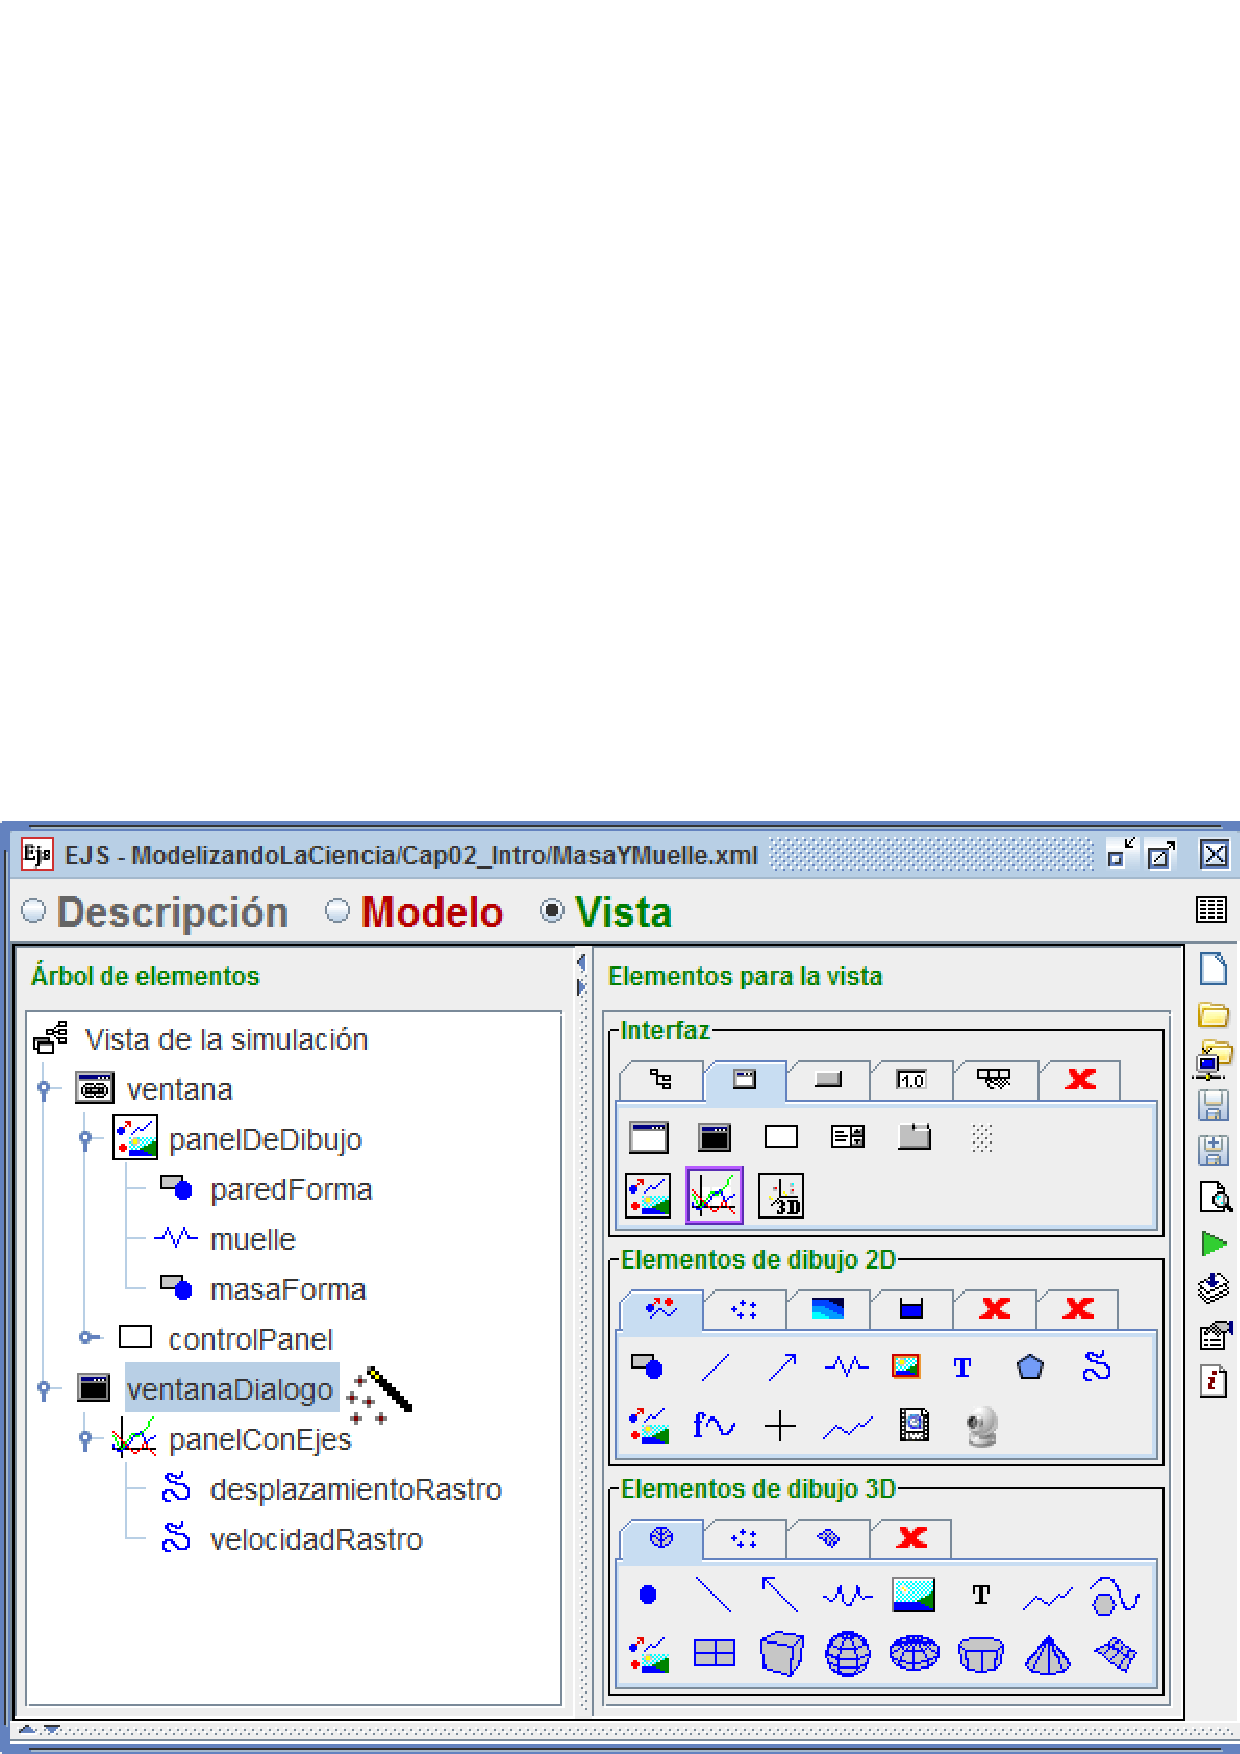
\includegraphics[scale=\scale]{02ExplorationJava/images/ModifyViewAddPlottingPanel.png}
    \caption{Creation of a plotting panel as a child of the \code{dialog} element of the view.}
    \label{fig:02ExplorationJava/ModifyViewAddPlottingPanel}
\end{figure}

\ejs\ asks for the name of the new element and then creates the element as a child within the existing \code{dialog}. A
new plot appears but the dialog is too small.  Resize the dialog box by dragging its
corner. You can also resize the dialog box by double-clicking on the \code{dialog} element in the tree to show its
properties table and changing its \code{Size} property to \code{"385,524"}, thus doubling its height. Finally, edit the
properties table of the newly created plotting panel element to set the \code{Title} property to \code{Phase Space},
the \code{Title X} property to \code{Displacement}, and the \code{Title Y} property to \code{Velocity}. (\ejs\ will
add leading and trailing quotes to these strings to conform to the correct Java syntax.) Set the minima
and maxima for both X and Y scales to \code{-1} and {1}, respectively, and leave the other properties untouched.

The plotting panel is, as its name suggests, the container for the phase-space plot. Phase space data are drawn in this
panel using an element of type \code{Trail2D}, 
\includegraphics[scale=\linescale]{../_common/icons_png/Elements/Trail.png}.  Find the
\code{Trail2D} element in the \code{2D Drawables} palette and follow the same procedure as before.  Select the
\code{Trail2D} element and create an element of this type by clicking with the magic wand on the phase space panel.
Finally, edit the properties of the new trail element to set its \code{Input X} property to \code{x - L} and its
\code{Input Y} property to \code{vx}. This assignment causes the simulation to add a new \code{(x - L,vx)} point to the
trace after each evolution step, thus drawing the phase-space plot shown in Figure~\ref{fig:02ExplorationJava/ModifyRunning}.

\begin{figure}[htb]
  \centering
  \includegraphics[scale=\scale]{02ExplorationJava/images/ModifyRunning.png}
  \caption{The modified simulation. The dialog includes now both a time and a phase-space plot.}
  \label{fig:02ExplorationJava/ModifyRunning}
\end{figure}

To finish the modifications, we add a new panel to the top of the drawing frame that shows the sinusoidal driving force parameters.

\begin{bulletlist}

\item Select the \code{Panel} element icon, 
\includegraphics[scale=\linescale]{../_common/icons_png/Elements/Panel.png}, on the \lit{Windows, containers, and drawing panels} subgroup of the \lit{Interface} palette. Click with the magic wand on the element named \code{frame} within the \lit{Tree of elements} to create a new panel named \code{forceParamPanel} in the frame's top location. Use the properties inspector to set this panel's layout to \lit{FLOW:center,0,0} and its border type to \texttt{LOWERED\_ETCHED}.
\item Select the \code{Label} element icon, 
\includegraphics[scale=\linescale]{../_common/icons_png/Elements/Label.png}, on the \lit{Buttons and decorations} subgroup of the \lit{Interface} palette and create a new element of that type in the \code{forceParamPanel} panel.  Set the label's text property to \texttt{"frequency ="}.
\item Select the \code{Field} element icon, 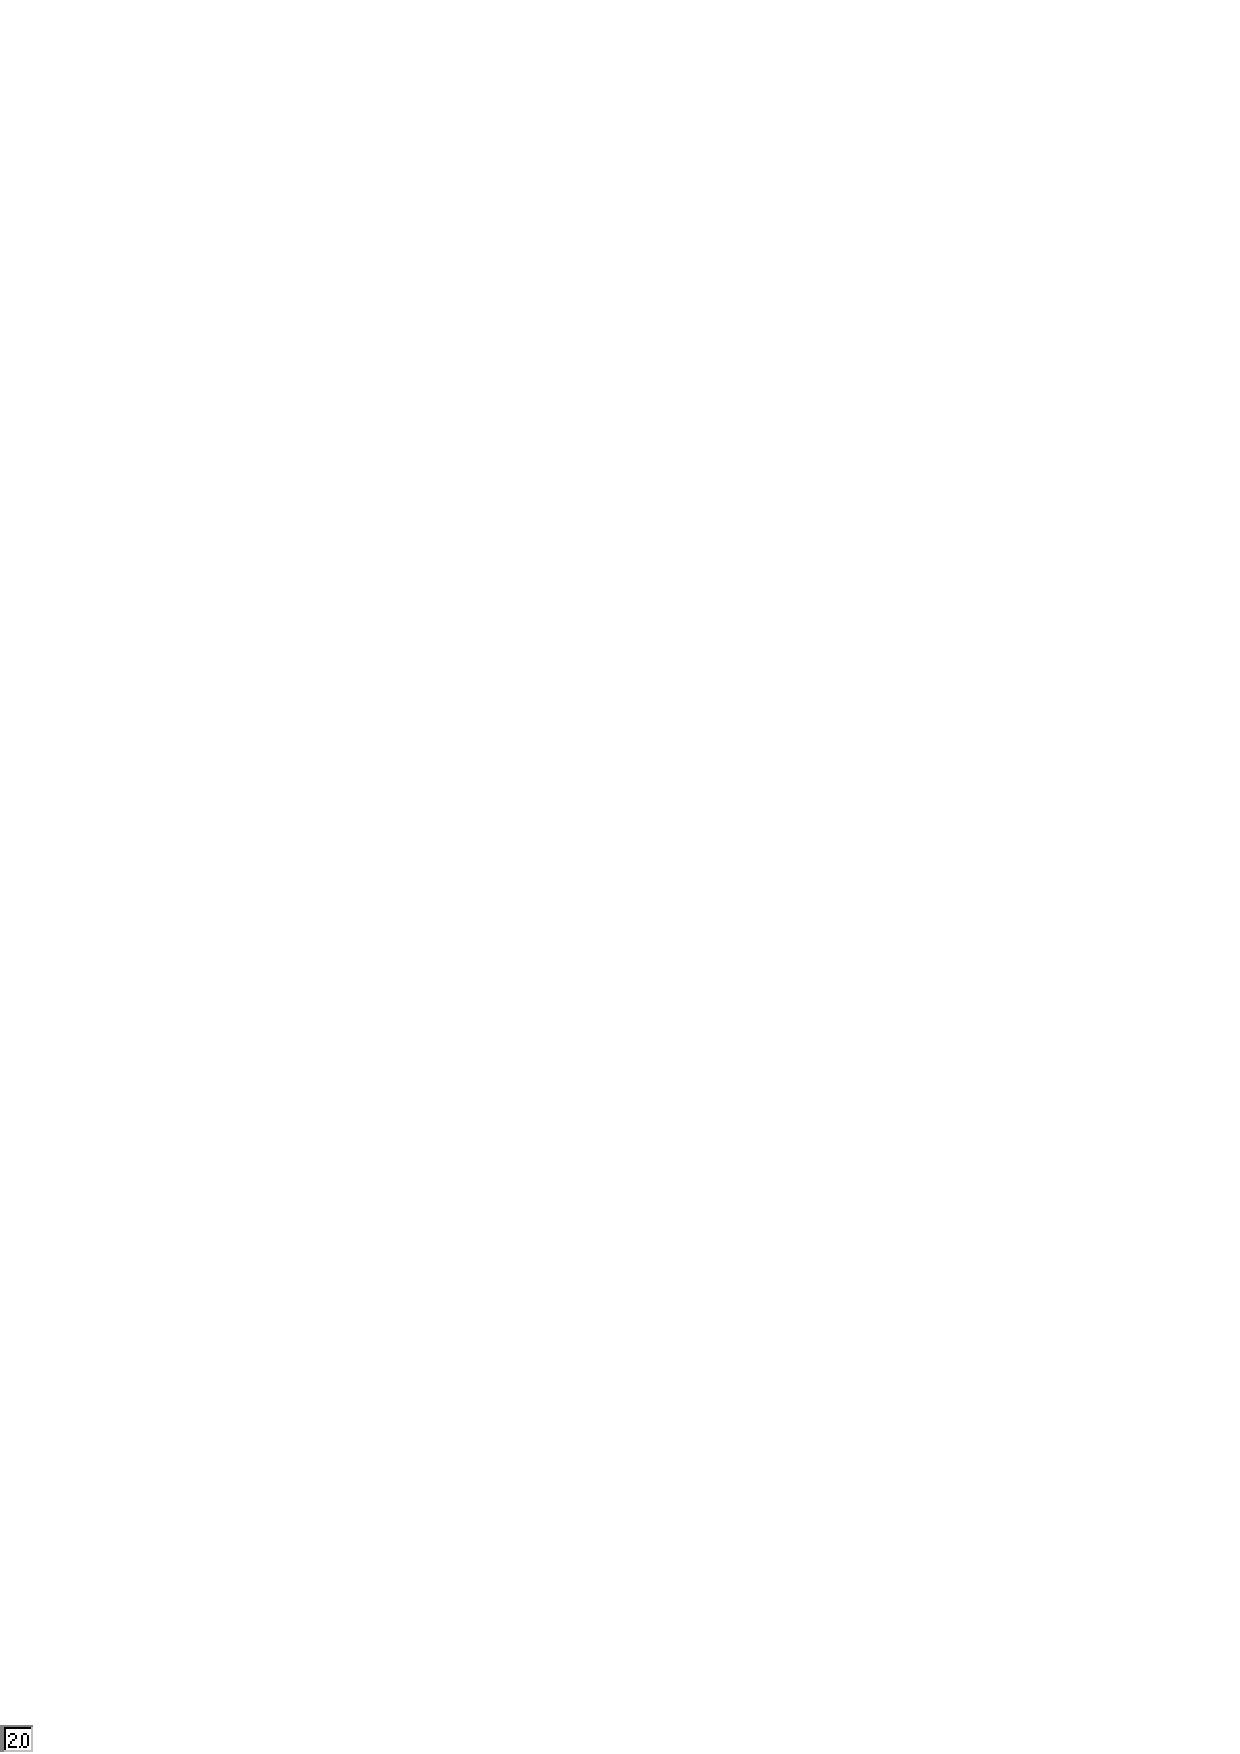
\includegraphics[scale=\linescale]{../_common/icons_png/Elements/ParsedField.png}, and create a new element named \code{freqField} in the force parameter panel.  Edit the \code{freqField} properties table as shown in Figure~\ref{fig:02ExplorationJava/ModifyField}. The connection to the \code{freq} variable is established using the \code{Variable} property.  Click on the second icon to the right of the property field, 
\includegraphics[scale=\linescale]{../_common/icons_png/link.png}, and choose the appropriate variable. The variable list shows all the model variables that can be used to set the property field. The \code{Format} property indicates the number of decimal digits with which to display the value of the variable.
\item Repeat this process to add the \code{amp} variable to the user interface.
\end{bulletlist}

\begin{figure}[htb]
    \centering
  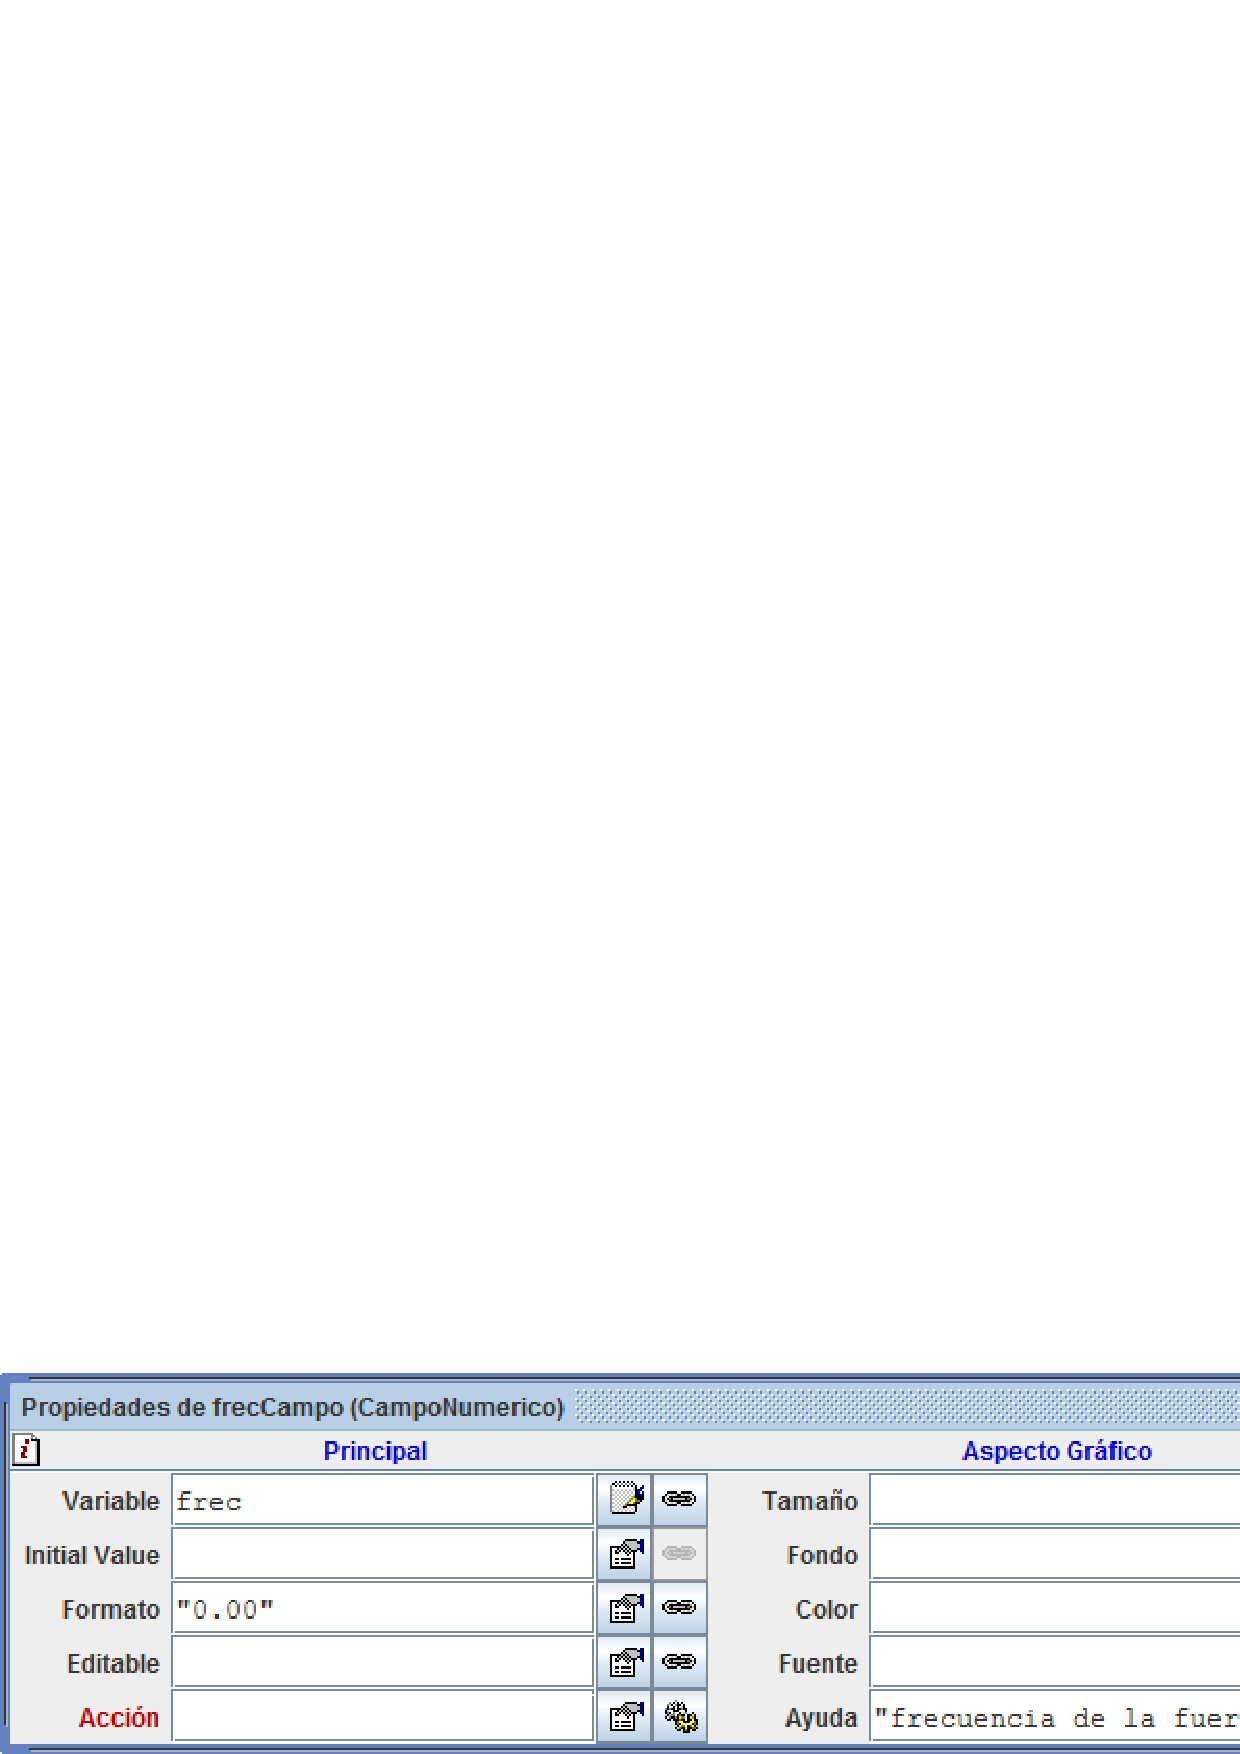
\includegraphics[scale=\scale]{02ExplorationJava/images/ModifyField.png}
    \caption{The table of properties of the \code{freqField} element.}
    \label{fig:02ExplorationJava/ModifyField}
\end{figure}

\subsection{Changing the description}\label{section:02ExplorationJavaModifyingDescription}

Now that we have changed the model and the view, we should modify the description pages of our simulation. Go to the \lit{Description} workpanel and click on the tab of the first page, the one labeled \code{Introduction}. Once you see this page, click the \lit{Click to modify the page} icon, 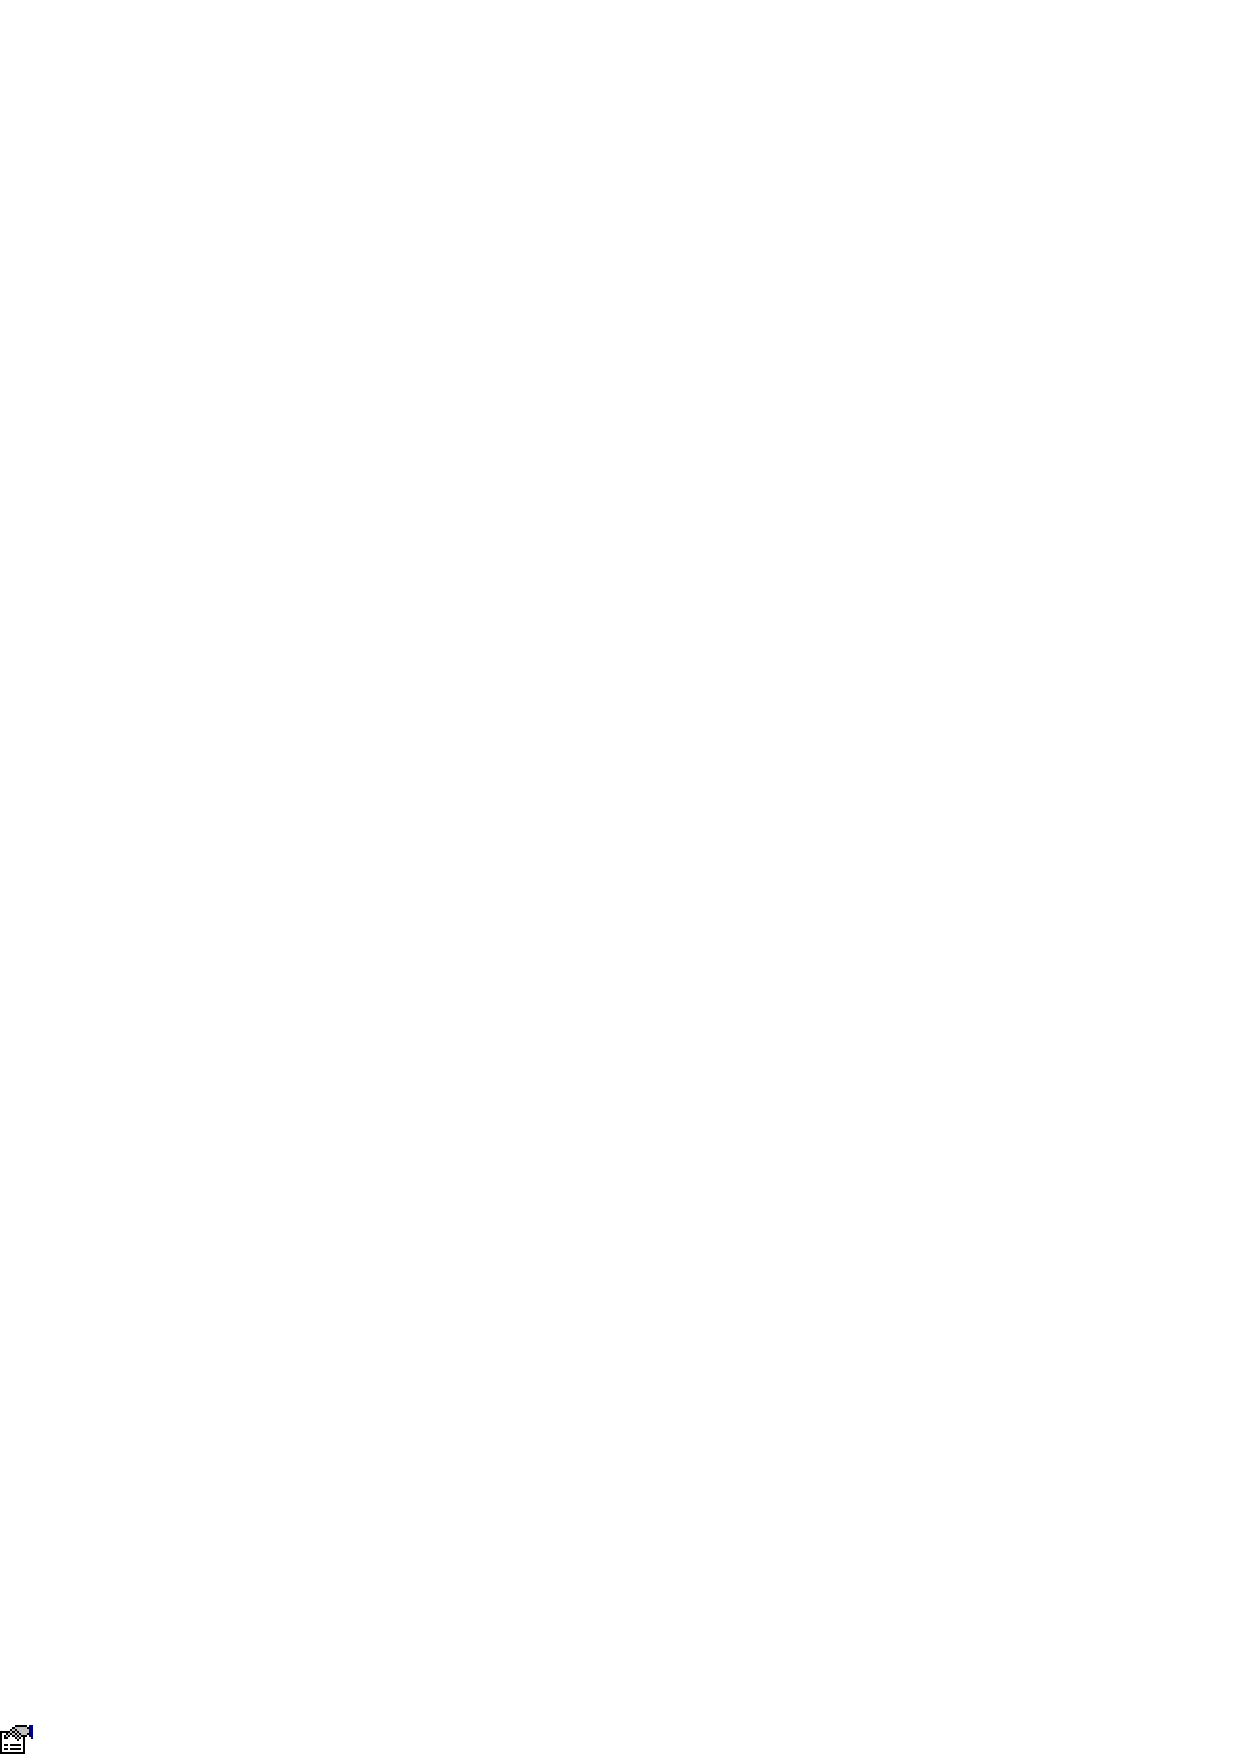
\includegraphics[scale=\linescale]{../_common/icons_png/edit.png}. The description page will change to edit mode, as shown in Figure~\ref{fig:02ExplorationJava/ModifyHTML}, and a simple editor will appear that provides direct access to common HTML features.

If you prefer to use your own editor, you can copy and paste HTML fragments from your editor into the \ejs\ editor. If you know HTML syntax, you can enter tagged (markup) text directly by clicking the source icon, 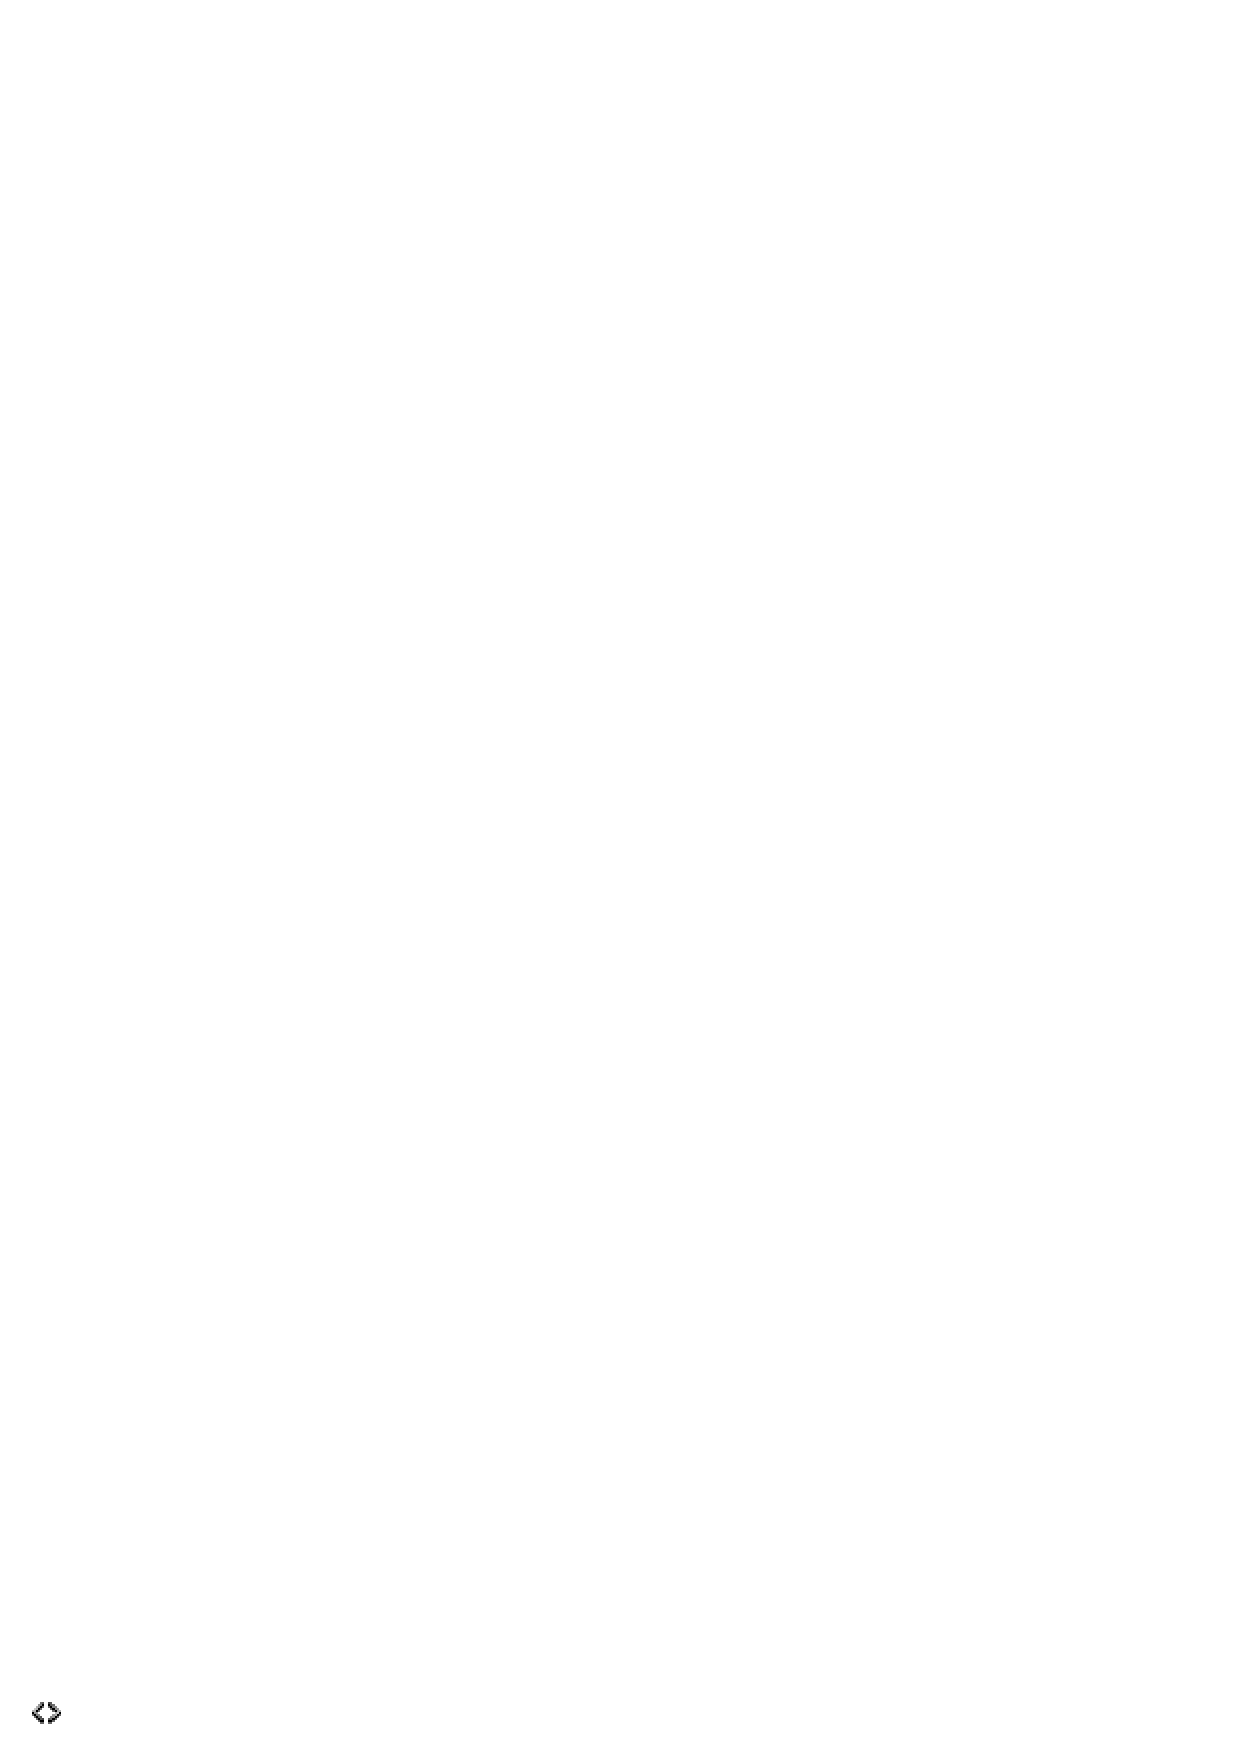
\includegraphics[scale=\linescale]{02ExplorationJava/images/SourceHK.png}, in the tool bar.  You can even import entire HTML pages into \ejs\ by clicking the \lit{Link/Unlink page to external file} icons, 
\includegraphics[scale=\linescale]{../_common/icons_png/link.png}, \includegraphics[scale=\linescale]{../_common/icons_png/unlinked.png}.

\begin{figure}[htb]
    \centering
  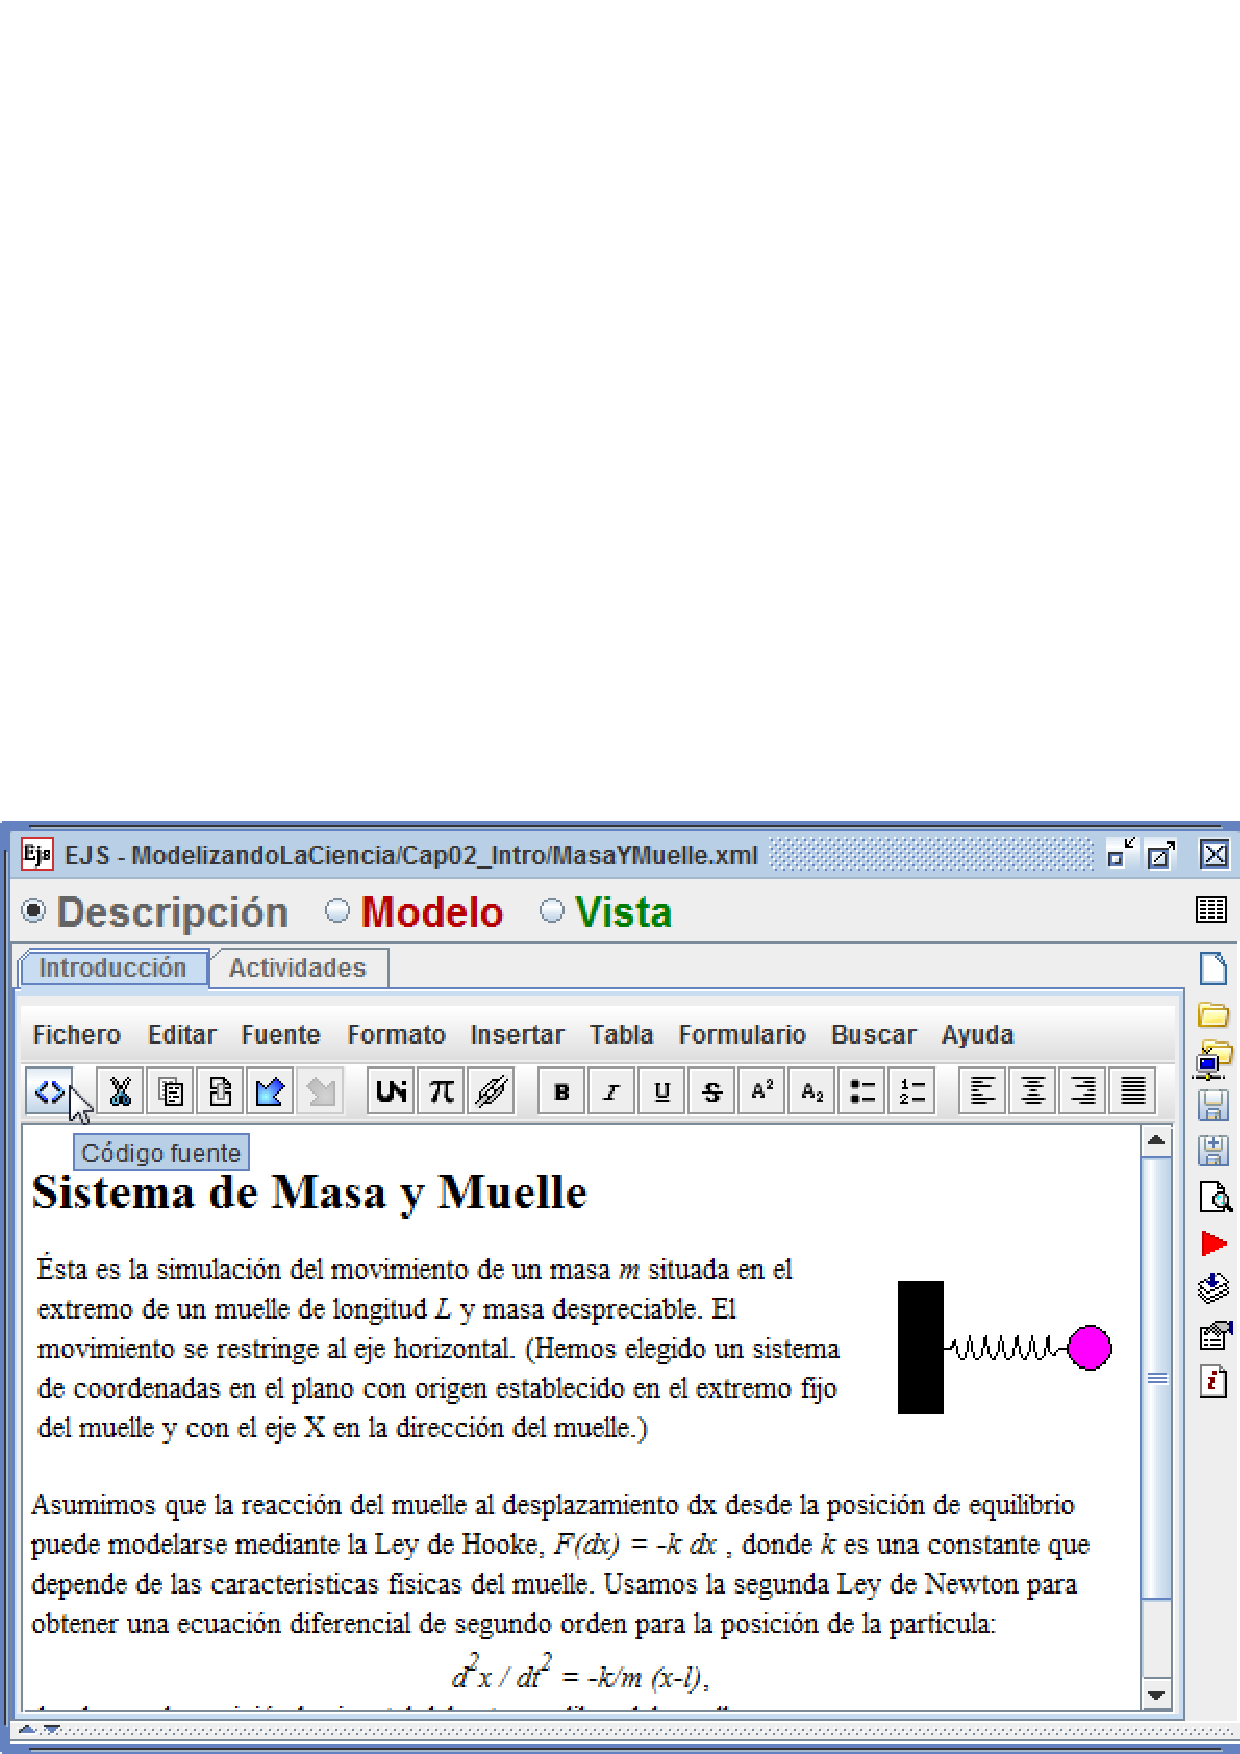
\includegraphics[scale=\scale]{02ExplorationJava/images/ModifyHTML.png}
    \caption{The HTML editor of \ejs. The added red arrows point to the edit and source code edition mode icons.}
    \label{fig:02ExplorationJava/ModifyHTML}
\end{figure}

Edit the description pages as you find convenient. At least change the discussion of the model to include the damping and driving forces. When you are done, save the new simulation with a different name by clicking the \lit{Save as} icon of \ejs' taskbar, 
\includegraphics[scale=\linescale]{../_common/icons_png/saveAsSmall.png}. When prompted, enter a new name for your simulation's XML file. The modified simulation is stored in the \file{MassAndSpringComplete.ejs} file in the \file{source} directory for this chapter.

% -----------------------------------------------------
\section{Problems and Projects}\label{section:02ExplorationJavaProjects}
% -----------------------------------------------------

%\subsection*{Problem 1}
\begin{problem}[Energy]
Add a third plotting panel to the dialog window of the \file{MassAndSpringComplete.ejs} simulation that will display the evolution of the kinetic, potential, and total energies.
\end{problem}

%\subsection*{Problem 2}
\begin{problem}[Function plotter]
The analytic solution for the undriven simple harmonic oscillator is
\begin{equation}
  x(t)=A \sin(w_0 t + \phi)
\end{equation}
where $A$ is the amplitude (maximum displacement), $w_0= \sqrt{k/m}$ is the natural frequency of oscillation, and
$\phi$ is the phase angle.  Consult a mechanics textbook to determine the relationship between the amplitude and phase
angle and the initial displacement and velocity.  Use the \file{FunctionPlotter.ejs} simulation in the
examples directory to compare the analytic solution to the numerical solution generated by the
\file{MassAndSpringComplete.ejs} model.
\end{problem}

%\subsection*{Project 2}
\begin{project}[Two-dimensional oscillator]
Modify the model of the mass and spring simulation to consider motion that is not restricted to the horizontal
direction.  Assume that a second spring with spring constant $k'$ produces a vertical restoring force $F_y(\delta y) = - k' \,\delta y$. Modify the simulation to allow the user to specify the Hooke's law constants as well as the initial conditions in both directions. Describe the motion produced without a driving force but under different initial conditions and with different spring constants. (Try $k=1$ and $k'=9$.)  Show that it is possible to obtain circular motion if $k=k'$.
\end{project}

%\subsection*{Project 3}
\begin{project}[Simple pendulum]
Create a similar simulation as the one described in this chapter for a simple pendulum whose second-order differential
equation of motion is
\begin{equation}
  \frac{d^2\theta}{dt^2} = -\frac{g}{L} \sin (\theta),
\end{equation}
where $\theta$ is the angle of the pendulum with the vertical, $g$ is the acceleration due to gravity, and $L$ is the arms's length. Use fixed relations to compute the $x$ and $y$ position of the pendulum bob using the equations:
\begin{align*}
   x   &=  L \, \sin (\theta) \\
   y   &= -L \, \cos (\theta).
\end{align*}
\end{project}
          % Chapter: Introduction to Ejs
      % !TEX root = ../Guide de l'utilisateur de EjsS.tex

\chapter{Examiner l'ar�me Javascript de  \Ejs}\label{chapter:JavascriptEJS}

\begin{quote}
Le changement est la loi de la vie. Et ceux dont le regard est tourn� vers le pass� ou le pr�sent sont certains de rater l'avenir. {\em John F. Kennedy}
\end{quote}

Pour offrir une perspective du processus de mod�lisation nous allons, dans ce chapitre, premi�rement  ouvrir, examiner et  ex�cuter une simulation d'un oscillateur harmonique simple existant. Par la suite, nous allons modifier la simulation pour montrer comment \ejs\ engage l'utilisateur dans le processus de mod�lisation et r�duit  en grande partie la quantit� de programmation qui est n�cessaire. Le chapitre utilise JavaScript  comme langage de programmation pour la mod�lisation et c'est un chapitre similaire au Chapitre~\ref{chapter:JavaEJS} (dans lequel Java est utilis�).

% ------------------------
    \section{Examiner la simulation}\label{section:03ExplorationJavascriptInspecting}\index{\Ejs!inspecting a simulation}
% ------------------------

Comme nous l'avons mentionn� dans le Chapitre~\ref{chapter:EjsIntro}, \Ejs\ fournit trois panneaux de travail pour construire des  simulations. Le premier panneau, \lit{Description}, nous permet de cr�er et d'�diter un texte multim�dia bas� sur HTML qui d�crit la simulation.\index{HTML}  
Le deuxi�me panneau, \lit{Model,} est d�di� au processus de mod�lisation. Nous utilisons cet espace pour cr�er des variables qui d�crivent le mod�le, pour initialiser ces variables et pour �crire des algorithmes qui d�crivent comment ce mod�le change dans le temps. Le troisi�me panneau, \lit{HtmlView}, est d�di� � la t�che d' �laborer l'interface graphique utilisateur qui permet � l'utilisateur de contr�ler la simulation et d'afficher les r�sultats ou donn�es de sortie. 

Pour comprendre comment les panneaux \lit{Description}, \lit{Model} et \lit{HtmlView}  fonctionnent collaborativement, nous allons examiner et ex�cuter une simulation existante. Une capture d'�cran ne remplace pas une d�monstration en direct et nous vous encourageons � continuer � suivre sur votre ordinateur au fur et mesure que vous lisez. 

Cliquez sur l'ic�ne \lit{Open} icon, 
\includegraphics[scale=\linescale]{../_common/icons_png/openSmall.png},  de la barre de t�che de \ejs. Une bo�te de dialogue de fichier similaire � celle qui est sur la figure~\ref{fig:03ExplorationJavascript/OpenDialog}   s'affiche pour montrer le contenu du r�pertoire \file{source} de votre environnement de travail. Dirigez-vous sur le r�pertoire \file{JavascriptExamples} o� vous trouverez un fichier intitul� \file{MassAndSpring.ejss}. S�lectionnez ce fichier et cliquez sur le bouton \lit{Open} de la bo�te de dialogue. 

\begin{figure}[htb]
  \centering
  \subfigure{\includegraphics[scale=0.2]{03ExplorationJavascript/images/OpenDialogCrossPlatform.png}}
  \subfigure{\includegraphics[scale=0.2]{03ExplorationJavascript/images/OpenDialogNative.png}}  
  \caption{La bo�te de dialogue de fichier ouverte vous permet de naviguer sur votre disque dur et de ouvrir une simulation existante. L'apparence de la bo�te de dialogue (deux types diff�rents de \lit{look and feels} -- pr�sentations -- sont affich�s ici) peut varier en fonction de votre syst�me d'exploitation et de la pr�sentation s�lectionn�e. \label{fig:03ExplorationJavascript/OpenDialog}}
\end{figure}

Maintenant les choses deviennent r�elles! \ejs\ lit le document \file{MassAndSpring.ejss} qui comble le panneau et un navigateur intitul� ``EjsS- PREVIEW'' appara�t sur votre �cran comme indiqu� dans la figure~\ref{fig:03ExplorationJavascript/SpringInterface}.~\footnote{Si le navigateur n'appara�t pas, de-s�lectionnez la case � cocher  \lit{Keep preview hidden} (Garder la pr�visualisation cach�e) du panneau \lit{HtmlView}.}
 Un petit avertissement. Vous pouvez d�placer les objets et cliquer sur des boutons de la maquette de la fen�tre mais le mod�le ne repr�sentera pas le comportement complet. Pour cela vous devez ex�cuter la simulation.

\begin{figure}[htb]
  \centering
  \includegraphics[scale=\scale]{03ExplorationJavascript/images/SpringInterface.png}
  \caption{La maquette de fen�tre de \ejs\ de la simulation \file{MassAndSpring}. La barre de titre et la bordure rouge indique que c'est une page de pr�visualisation  HTML et que le programme ne s'ex�cute pas.}
  \label{fig:03ExplorationJavascript/SpringInterface}
\end{figure}

\note{Les lecteurs impatients ou pr�coces peuvent �tre tent�s de cliquer sur l'ic�ne vert d'activation \includegraphics[scale=\linescale]{../_common/icons_png/launch.png} de la barre de t�ches pour ex�cuter notre exemple avant de proc�der avec le tutoriel. Les lecteurs qui feront cela n'interagiront plus directement avec \ejs,  mais avec un programme complet d'ex�cution de JavaScript sur une nouvelle page HTML.  Quittez le programme d'ex�cution en fermant ce nouveau page web \lit{Mass and Spring} avant de proc�der.}

\subsection{The panneau \lit{Description}}

S�lectionnez le panneau \lit{Description}\index{Ejs!Description}  en cliquant sur le bouton radio correspondant dans la partie sup�rieure de \ejs\  et vous verrez deux pages de texte pour cette simulation. La premi�re page affich�e dans la figure~\ref{fig:03ExplorationJavascript/SpringDesc} contient un petit d�bat sur le mod�le de masse-ressort. Cliquer sur la barre \lit{Activities} (activit�s) pour voir le deuxi�me texte. 

\begin{figure}[htb]
  \centering
  \includegraphics[scale=\scale]{03ExplorationJavascript/images/SpringDesc.png}
  \caption{Les pages de description pour la simulation de la masse-ressort. Cliquez sur la barre pour afficher la page. Faites un clic-droit sur la barre pour �diter la page.}
  \label{fig:03ExplorationJavascript/SpringDesc}
\end{figure}

Une \lit{Description} est un texte multim�dia HTML\index{HTML}  ou XHTML\index{XHTML} qui fournit de l'information et des instructions sur la simulation.  HTML repr�sente Hypertext Markup Language (langage de balisage d'hypertexte) et c'est le protocole le plus habituellement utilis� pour le formatage et l'affichage de documents sur le Web. Le X de XHTML signifie eXtensible. XHTML est essentiellement un HTML exprim� comme un XML valide ou, d'un mode plus simple,  un HTML parfaitement format�.

\ejs\  fournit un �diteur HTLM simple qui vous permet de cr�er et de modifier des pages sur \ejs. Vous pouvez aussi importer des pages HTML ou (pr�f�rablement) XHTML � \ejs\  en faisant un clic droit sur la barre de l'espace de travail \lit{Description}.  (Voir la Section~\ref{section:03ExplorationJavascriptModifyingDescription}.) Les pages de description sont une partie essentielle du processus de mod�lisation et ces pages sont inclus dans le mod�le compil� quand le mod�le est export� pour sa distribution.


\subsection{Le panneau \lit{Model}}\label{section:03ExplorationJavascriptModel}

Le panneau \lit{Model} est l'espace o� le mod�le est d�fini pour qu'il puisse �tre converti en un programme par \ejs. Dans cette simulation, nous �tudions le mouvement de la particule de masse m attach� � une extr�mit� du ressort sans masse de la longueur d'�quilibre $L$.

 Le ressort est fix� au mur par son autre extr�mit� et son mouvement est restreint en direction horizontale. Bien que la masse oscillante pr�sente une solution analytique bien connue, il est utile de commencer par le mod�le oscillateur harmonique simple pour que nos donn�es de sortie puissent �tre compar�es avec le r�sultat analytique exact. \index{Simple Harmonic Motion}
 
Notre mod�le assume des petites oscillations pour que le ressort r�ponde � un d�placement donn� horizontal $\delta x$ de la longueur de l'�quilibre $L$ sous une force d�termin�e par la Loi de Hooke,\index{Hooke's law} $F_x = - k \,\delta x$, dans laquelle $k$ est la constante �lastique du ressort, qui d�pend de ses caract�ristiques physiques. Nous utilisons la deuxi�me Loi de Newton\index{Newton's second law} pour obtenir une �quation diff�rentielle du second ordre pour la position de la particule:
\begin{equation}
  \frac{d^2\ x}{dt^2} = -\frac{k}{m}\,(x-L). \label{eq:03ExplorationJavascript/SpringBasic}
\end{equation}
 Remarquez que nous utilisons un syst�me de coordonn�es avec l'axe-$x$  au long du ressort et son origine est � l'extr�mit� du ressort qui est fix�e. La particule est plac�e �  $x$ et le d�placement de l'�quilibre  $\delta x=x-L$ �quivaut � z�ro quand $x=L$ . Nous r�solvons ce syst�me num�riquement pour �tudier l'�volution de son �tat dans le temps.
 
Voyons comment nous allons impl�menter le mod�le de masse-ressort en s�lectionnant le bouton radio de \lit{Model} et en examinant chacun des six panneaux.

\subsubsection{D�claration des variables }
\begin{figure}[htb]
    \centering
  \includegraphics[scale=\scale]{03ExplorationJavascript/images/ModelVariables.png}
    \caption{
    Le panneau  \lit{Model} contient six sous-panneaux de travail. Le sous-panneau pour la d�finition des variables dynamiques masse-ressort est affich�. D'autres onglets dans ce sous-panneau de travail d�finissent les variables additionnelles telles que la longueur naturelle du ressort $L$ et l'�nergie $E$. } 
    \label{fig:03ExplorationJavascript/ModelVariables}
\end{figure}

Quand vous impl�mentez un mod�le, une des bonnes choses � faire premi�rement c'est identifier, d�finir et initialiser les variables qui d�crivent le syst�me. Le terme \emph{variable} est tr�s g�n�ral et fait r�f�rence � tout ce que l'on peut attribuer un nom, y compris une constante physique et un graphique.\index{Model!Variables} La figure~\ref{fig:03ExplorationJavascript/ModelVariables} affiche un panneau de variable \ejs. Chaque ligne d�finit une variable du mod�le en pr�cisant le nom de la variable, le type, la dimension et la valeur initiale.

 Les variables dans les programmes informatiques peuvent �tre de diff�rents types en fonction de l'information qu'elles d�tiennent. Les types plus habituellement utilis�s sont  \code{boolean} pour les valeurs vrai/faux, \code{int} pour les nombres entiers, \code{double} pour les valeurs num�riques � haute pr�cision ($\approx 16$ chiffres significatifs) et  \code{String} pour les textes. Nous utiliserons tous ces types de variables dans ce document mais le mod�le masse-ressort utilise seulement les variables de type  \code{double} et \code{boolean}.


\note{Si vous avez d�j� appris un peu de JavaScript, vous saurez probablement que JavaScript n'a aucun type pour les variables. Toutes les variables sont d�clar�es avec un mot-cl� \code{var}. Ce qui veut dire que, en principe, JavaScript ne fait aucune diff�rence entre integers (les nombres entiers), double (les nombres � haute pr�cision) ou String (les textes), etc\ldots  Mais il le fait! Par exemple vous ne devez pas utiliser une  variable double comme index pour un tableau (\emph{array}, en anglais). C'est pour cela et parce qu'il vous aide � clarifier l'utilisation des variables dans votre mod�le (quelles valeurs elles peuvent d�tenir et o� vous pouvez ou vous ne pouvez pas les utiliser) nous vous recommandons d'attribuer un type � chaque variable de votre mod�le.}

Les variables peuvent s'utiliser comme param�tres, \index{Model!Parameters} comme variables d'�tat \index{Model!State variables} ou comme donn�es d'entr�e et de sortie du mod�le.\index{Model!Input and Output} Les panneaus de la figure~\ref{fig:03ExplorationJavascript/ModelVariables}  d�finissent les variables utilis�es dans notre mod�le. Nous avons d�clar� une variable pour la position-$x$  de la particule, \code{x}, pour sa vitesse dans la direction-$x$, \code{vx}, pour le temps, \code{t}, et pour l'incr�ment de temps � chaque �tape de la simulation, \code{dt}. Nous d�finissons quelques variables dans cet onglet et dans d'autres qui n'apparaissent pas dans l'equation\eqref{eq:03ExplorationJavascript/SpringBasic}. Les raisons pour l'utilisation de variables auxiliaires telles que \code{vx}  ou les �nergies cin�tiques, potentielles ou totales seront indiqu�es clairement par la suite. La partie inf�rieure du panneau de variables contient un champ de commentaires qui fournit une description du r�le de chaque variable dans le mod�le. Cliquez sur une variable pour afficher le commentaire correspondant.


\subsubsection{Initialisation du mod�le}
Fixer les conditions initiales correctement est tr�s important quand vous impl�mentez un mod�le car le mod�le doit commencer dans un �tat qui puisse se r�aliser physiquement. Notre mod�le est relativement simple et nous l'initialisons en introduisant des valeurs (ou des expressions simples de JavaScript telles que \code{0.5*m*vx*vx}) dans la colonne \lit{Initial value} (valeur initiale) du panneau de variables. \ejs\  utilise ces valeurs quand il initialise la simulation.


\note{Les mod�les avanc�s peuvent n�cessiter un algorithme d'initialisation. Par exemple un mod�le dynamique mol�culaire peut fixer la vitesse de chaque particule pour un ensemble de particules. Le panneau \lit{Initialization} nous permet de d�finir une ou plusieurs pages de code JavaScript qui r�alisent les calculs n�cessaires. \ejs\  transforme ce code en une fonction JavaScript\index{Javascript!function} et reprend cette fonction au d�marrage et chaque fois que la simulation est r�initialis�e. Le panneau \lit{Initialization}  de masse-ressort n'est pas affich� parce qu'il est vide. Voir le Paragraphe~\ref{section:03ExplorationJavascriptInspectingRelations} pour un exemple de comment le code JavaScript appara�t sur \ejs.}


\subsubsection{L'�volution du mod�le}

Le panneau \lit{Evolution} nous permet d'�crire le code JavaScript qui d�termine comment le syst�me masse-ressort �volue dans le temps et il utilisera cette option fr�quemment pour les mod�les qui ne sont pas bas�s sur des �quations diff�rentielles ordinaires (EDO, ODE en anglais). Cependant, il y a une deuxi�me option qui nous permet d'introduire des �quations diff�rentielles ordinaires telles que \eqref{eq:03ExplorationJavascript/SpringBasic} sans programmer. \ejs\ fournit un �diteur d�di� qui nous permet de pr�ciser des �quations diff�rentielles dans un format qui ressemble � des notations math�matiques et qui g�n�re automatiquement le code JavaScript correct.

Voyons comment l'�diteur d'�quations diff�rentielles fonctionne pour le mod�le de masse-ressort. �tant donn� que les algorithmes EDO r�solvent des syst�mes d'�quations diff�rentielles ordinaires de premier ordre, une �quation d'ordre sup�rieur tel que \eqref{eq:03ExplorationJavascript/SpringBasic} doit �tre refond�e dans un syst�me de premier ordre. Nous pouvons faire cela en consid�rant la vitesse comme une variable ind�pendante qui ob�it � sa propre �quation:
\begin{align}
  \frac{d\ x} {dt} &= v_x                           \label{eq:03ExplorationJavascript/SpringBasicODE1} \\
  \frac{d\ v_x}{dt} &= -\frac{k}{m}\,(x-L). \label{eq:03ExplorationJavascript/SpringBasicODE2}
\end{align}
La n�cessit� d'une �quation diff�rentielle additionnelle explique pourquoi nous d�clarons la variable \code{vx}  dans notre panneau de variables.

 En cliquant sur le panneau \lit{Evolution}, l'�diteur EDO repr�sent� dans la figure~\ref{fig:03ExplorationJavascript/ModelEvolution} s'affiche.
 
\begin{figure}[htb]
    \centering
  \includegraphics[scale=\scale]{03ExplorationJavascript/images/ModelEvolution.png}
    \caption{Le panneau �volution ODE (EDO en fran�ais) repr�sente l'�quation diff�rentielle  et l'algorithme num�rique de la masse-ressort.}
    \label{fig:03ExplorationJavascript/ModelEvolution}
\end{figure}
Remarquez que l'�diteur EDO affiche \eqref{eq:03ExplorationJavascript/SpringBasicODE1} et \eqref{eq:03ExplorationJavascript/SpringBasicODE2} (en utilisant le caract�re \lit{*} pour d�signer la multiplication). Les champs qui se trouvent dans la partie sup�rieure de l'�diteur pr�cisent la variable ind�pendante \code{t} et l'incr�ment de variable \code{dt}. Les algorithmes num�riques estiment la solution EDO exacte en indiquant l'�tat dans les �tapes distinctes et l'incr�ment d�termine cette intervalle. Le bouton \lit{Prelim code} dans la partie sup�rieure droite de l'�diteur nous permet d'introduire un code pr�liminaire pour r�aliser les calculs avant d'�valuer les �quations (une circonstance n�cessaire dans des situations plus complexes que celle dont nous nous occupons dans cet exemple). Un menu d�roulant dans la partie inf�rieure de l'�diteur nous permet de s�lectionner le \emph{solutionneur} EDO, un algorithme num�rique qui anticipe la solution � partir de la valeur actuelle de temps, \code{t} � la suivante valeur \code{t+dt}. Le champ de tol�rance (\lit{Tol}) est gris� et vide car Runge-Kutta 4 est une m�thode � �tape fixe qui ne n�cessite pas de param�tres de tol�rance. Le bouton \lit{Fine-tune\ldots} affiche un dialogue  qui nous permet de r�gler l'ex�cution de ce solutionneur bien que les valeurs par d�faut soient normalement appropri�es. Finalement le champ d'�v�nements (\lit{Events}) dans la partie inf�rieure du panneau nous indique que nous n'avons d�fini aucun �v�nement pour cette �quation diff�rentielle. Vous pourrez trouver des exemples avec des codes pr�liminaires et des �v�nements dans les pages suivantes de ce document. Les diff�rents algorithmes de r�solution et leurs param�tres sont comment�s dans la bulle d'aide de \ejs.

La partie gauche de l'espace de travail evolution comprend des champs qui d�terminent � quel niveau de \emph{douceur} et � quelle vitesse la simulation s'ex�cute. L'option de \lit{frames per second} (\lit{FPS}) --- images par seconde --- qui peut �tre s�lectionn�e soit en utilisant un curseur, soit un champ de saisie, pr�cise combien de fois par seconde nous voulons que notre simulation soit redessin�e sur l'�cran. Le champ de saisie \lit{steps per display} (\lit{SPD})  --- �tape par affichage --- pr�cise combien de fois nous voulons faire progresser le mod�le avant de le redessiner. La valeur actuelle de \code{20} images par seconde produit une bonne animation qui, conjointement avec la valeur prescrite d'une �tape par affichage et \code{0.05} pour \code{dt},  donne lieu � une simulation qui s'ex�cute (� peu pr�s) en temps r�el. Nous utiliserons pratiquement toujours le param�tre par d�faut d'une �tape par affichage. N�anmoins il y a des situations dans lesquelles les donn�es de sortie graphique du mod�le utilisent une quantit� consid�rable de la puissance de traitement et au cours desquelles nous voulons acc�l�rer les calculs num�riques. Dans ce cas nous pouvons augmenter la valeur du param�tre d'�tape par affichage pour que le mod�le progresse plusieurs fois avant que la visualisation soit redessin�e. La case � cocher \lit{Autoplay} indique si la simulation doit d�marrer quand le programme  d�marre. Cette case est d�sactiv�e pour que vous puissiez changer les conditions initiales avant de d�marrer l'�volution.

Le panneau \lit{Evolution} g�re les aspects techniques du mod�le EDO de masse-ressort sans programmer. La simulation fait progresser l'�tat du syst�me en r�solvant num�riquement les �quations diff�rentielles du mod�le et en utilisant l'algorithme interm�diaire. L'algorithme passe de l'�tat actuel � un temps  \code{t}  � un nouvel �tat � un nouveau temps \code{t + dt} avant que la visualisation soit redessin�e. La simulation r�p�te cette �tape �volution \code{20} fois par seconde sur les ordinateurs ou dispositifs avec une puissance de traitement faible. La simulation peut s'ex�cuter plus lentement ou incorrectement sur des ordinateurs ou des dispositifs avec une puissance de traitement insuffisante ou si l'ordinateur est occup� mais il devrait fonctionner.

\note{ Bien que le mod�le masse-ressort puisse se r�soudre avec un simple algorithme EDO, notre biblioth�que de m�thodes num�riques contient des algorithmes tr�s sophistiqu�s et \ejs\ peut appliquer ces algorithmes � de grands syst�mes d'�quations diff�rentielles de vecteur avec ou sans �v�nements discontinus.}

\subsubsection{Relation entre les variables}\label{section:03ExplorationJavascriptInspectingRelations}
Toutes les variables d'un mod�le ne sont pas calcul�es en utilisant un algorithme du panneau Evolution. Les variables peuvent se calculer apr�s que l'�volution soit appliqu�e. Nous faisons r�f�rence aux variables qui sont calcul�es en utilisant l'algorithme evolution comme des variables d'�tat ou des variables dynamiques et nous faisons r�f�rence aux variables qui d�pendent de ces variables comme des variables auxiliaires ou de sortie. Dans le mod�le masse-ressort les �nergies cin�tiques, potentielles et totales du syst�me sont des variables de sortie parce qu'elles sont calcul�es � partir de variables d'�tat:
\begin{align}
  T &= \frac{1}{2} m {v_x}^2,     \label{eq:03ExplorationJavascript/SpringEnergy1} \\
  V &= \frac{1}{2} k (x-L)^2,     \label{eq:03ExplorationJavascript/SpringEnergy2} \\
  E &= T + V.                     \label{eq:03ExplorationJavascript/SpringEnergy3}
\end{align}
On dit qu'il existe des relations fixes entre les variables du mod�le. 

Le panneau \lit{Fixed relations} repr�sent� dans la figure~\ref{fig:03ExplorationJavascript/ModelRelations}  s'utilise pour �crire des relations fixes entre les variables. Remarquez la facilit� pour convertir \eqref{eq:03ExplorationJavascript/SpringEnergy1} jusqu'a \eqref{eq:03ExplorationJavascript/SpringEnergy3}  � travers de la syntaxe JavaScript. Assurez-vous d'utiliser le caract�re de multiplication \lit{*} et d'�crire un point-virgule � la fin de chaque �nonc� JavaScript. 

\begin{figure}[htb]
    \centering
  \includegraphics[scale=\scale]{03ExplorationJavascript/images/ModelConstraints.png}
    \caption{Les relations fixes pour le mod�le masse-ressort.}
    \label{fig:03ExplorationJavascript/ModelRelations}
\end{figure}

\noindent \textbf{Voil� une importante remarque!} Vous vous demandez peut-�tre pourquoi nous n'�crivons pas des expressions de relation fixe en incorporant une deuxi�me page de code apr�s la page ODE (EDO)  dans le panneau \lit{Evolution}. Apr�s tout, les pages �volution ex�cutent s�quentiellement et  une deuxi�me page d'evolution actualiserait correctement les variables de sortie apr�s chaque �tape\ldots La raison pour laquelle le panneau \lit{Evolution} ne doit pas �tre utilis� c'est parce que les relations fixes doivent \emph{toujours} se maintenir car il y a d'autres mani�res, telles que les actions de la souris, pour modifier les variables d'�tat. Par exemple, d�placer la masse change la variable $x$ et ce changement affecte l'�nergie. \ejs\  �value automatiquement les relations apr�s l'initialisation, apr�s chaque �tape d'�volution et chaque fois qu'il y ait une interaction de l'utilisateur avec l'interface de la simulation. C'est pour cela que c'est important que les relations fixes entre variables soient annot�es sur le panneau \lit{Fixed relations}.

\subsubsection{Les pages personnalis�es (\lit{Custom})}

 Il y a un cinqui�me panneau dans le panneau \lit{Model}  intitul�  \lit{Custom} (Personnalisation). Ce panneau peut s'utiliser pour d�finir des fonctions JavaScript qu'on veut utiliser dans le mod�le. Ce panneau est vide parce que notre mod�le actuel ne n�cessite pas de m�thodes additionnelles mais nous utiliserons ce panneau quand nous modifierons l'exemple masse-ressort dans la Section~\ref{section:03ExplorationJavascriptModifying}. Une fonction personnalis�e ne s'utilise pas � moins qu'elle soit explicitement indiqu�e par un autre panneau.
 
\subsubsection{Les �l�ments du mod�le}

 Le sixi�me et dernier sous-panneau du panneau \lit{Model} est intitul� \lit{Elements} et il vous fournit un acc�s aux biblioth�ques JavaScript externes en forme de ic�nes glisser-d�poser. Vous incorporez ces biblioth�ques � votre programme en glissant l'ic�ne correspondant � la liste des �l�ments Model � utiliser pour ce mod�le. Cela cr�e des objets JavaScript que vous pouvez utiliser dans votre code mod�le. Ce panneau est aussi vide pour ce mod�le parce que notre mod�le masse-ressort ne n�cessite pas de biblioth�ques JavaScript  additionnelles.
 
% ---------------------------------------------
\subsection{Le panneau \lit{HtmlView}}
% ---------------------------------------------

\lit{HtlmView}  est le troisi�me panneau de \Ejs. Ce panneau nous permet de cr�er une interface graphique bas�e sur HTML qui comprend la visualisation, l'interaction de l'utilisateur et le contr�le du programme avec un minimum de programmation. La figure~\ref{fig:03ExplorationJavascript/SpringInterface}  repr�sente un affichage bas�e sur HTML pour le mod�le de masse-ressort. S�lectionnez le bouton radio \lit{HtlmView} pour examiner comment un affichage bas� sur HTML est cr��.

 Le cadre de droite du panneau \lit{HtlmView} de \ejs\ repr�sent� dans la figure~\ref{fig:03ExplorationJavascript/View} contient une collection d'�l�ments d'affichage (\emph{view elements})\index{Ejs!HtmlView elements} bas� sur HTLM, regroup�s en base � leur fonctionnalit�. Les �l�ments d'affichage sont des blocs de construction qui peuvent se combiner pour former une compl�te interface utilisateur bas� sur HTLM, et chaque �l�ment d'affichage est un objet sp�cialis� avec une repr�sentation sur l'�cran. Pour afficher l'information d'un �l�ment d�termin�, cliquez sur son ic�ne et tapez la touche \lit{F1} ou faites un clic droit pour s�lectionner le menu \lit{Help} (aide) de l'objet. Pour cr�er une interface utilisateur, nous cr�ons un affichage HTML vide (imaginez-le comme une page blanche HTML) et incorporez les �l�ments tels que le panneau, les boutons, les graphiques\ldots en utilisant glisser-d�poser tel que d�crit dans la Section~\ref{section:03ExplorationJavascriptModifying}.

\begin{figure}[htb]
    \centering
  \includegraphics[scale=\scale]{03ExplorationJavascript/images/View.png}
    \caption{Le panneau \lit{HtlmView} repr�sentant le \lit{Tree of elements} ( l'arbre des �l�ments) pour l'interface utilisateur masse-ressort.}
    \label{fig:03ExplorationJavascript/View}
\end{figure}

Le  \emph{Tree of elements} (l'arbre des �l�ments) repr�sent� sur le c�t� gauche de la figure~\ref{fig:03ExplorationJavascript/View} affiche la structure de l'interface utilisateur masse-ressort. Remarquez que la simulation pr�sente trois panneaux principaux: \code{labelPanel}, \code{centerPanel} et \code{bottomPanel} (panneau �tiquette, panneau central et panneau inf�rieur) qui sont align�s verticalement sur la page HTML du navigateur. Ces trois panneaux appartiennent � la classe d'�l�ments \emph{Containers} (de conteneurs), dont le but principal est de regrouper (organiser) visuellement d'autres �l�ments sur l'interface utilisateur. L'arbre des �l�ments affiche des noms descriptifs et des ic�nes pour ces �l�ments. Faites un clic-droit sur un �l�ment de l'arbre pour obtenir un menu qui aidera l'utilisateur � changer cette structure. Alternativement, vous pouvez glisser et d�poser les �l�ments d'un conteneur dans un autre pour changer la relation parent-enfant ou dans un conteneur pour changer l'ordre des enfants. 

\note{Il y a des conditions pour qu'un conteneur accepte un �l�ment donn� comme enfant. Par exemple un panneau d'affichage en deux dimensions peut seulement accepter des �l�ments d'affichage en 2D.}

Chaque �l�ment d'affichage pr�sente une s�rie de param�tres internes, d�nomin�s \lit{Properties}\index{Ejs!view element properties} (propri�t�s) qui configurent l'apparence et le comportement de l'�l�ment. Nous pouvons �diter ces propri�t�s en faisant double-clic sur l'�l�ment de l'arbre pour afficher un panneau connu comme \emph{properties inspector} (le contr�leur des propri�t�s) Les propri�t�s d'apparence telles que la couleur sont souvent �tablies par une valeur constante tel que \code{"Red"} (rouge). Nous pouvons aussi utiliser une variable du mod�le pour fixer la propri�t� d'un �l�ment. Cette capacit� pour connecter (relier) une propri�t� � une variable sans programmer est l'aspect essentiel pour transformer notre affichage en une visualisation dynamique et interactive.

Voyons comment ce processus fonctionne dans la pratique. Faites double clic sur l'�l�ment \code{massShape} (le suffixe `Shape' -- forme -- que nous ajoutons au nom de l'�l�ment vous aide � savoir de quel type d'�l�ment il s'agit) dans l'arbre pour afficher le contr�leur de propri�t�s des �l�ments. Cet �l�ment est la masse qui est associ�e � l'extr�mit� libre du ressort. Le panneau de propri�t�s de \lit{massShape} apparait tel qu'il est repr�sent� dans la figure~\ref{fig:03ExplorationJavascript/SpringBallProperties}.

\begin{figure}[htb]
    \centering
  \includegraphics[scale=\scale]{03ExplorationJavascript/images/SpringBallProperties.png}
    \caption{Le panneau de propri�t�s de l'�l�ment  \code{massShape}.}
    \label{fig:03ExplorationJavascript/SpringBallProperties}
\end{figure}

Observez les propri�t�s qui ont une valeur constante d�termin�e. Les propri�t�s  \code{ShapeType}, \code{SizeX}, \code{SizeY}, et \code{FillColor}  produisent une ellipse d'unit� de grandeur \code{(0.2,0.2)} qui produit un cercle (colori� en couleur Magenta). Plus important encore, les propri�t�s \code{X} et \code{Y} de la forme sont reli�s aux variables  \code{x} et \code{y} du mod�le. Cette simple attribution �tablit une connexion bidirectionnelle entre le mod�le et l'affichage. Ces variables changent conform�ment le mod�le �volue et les formes suivent les valeurs  \code{x} et \code{y}. Si l'utilisateur glisse la forme � un nouvel emplacement, les variables \code{x} et \code{y} du mod�le changent en cons�quence. Remarquez cependant, que la propri�t� \code{Draggable} (glissable) est fix�e pour vous permettre uniquement de d�placer horizontalement la masse.

Les �l�ments peuvent aussi avoir des propri�t�s d'action\index{Ejs!action properties} qui peuvent s'associer � un code. (Les �tiquettes des propri�t�s d'actions sont affich�es en rouge.) Les actions de l'utilisateur telles que glisser ou cliquer, comporte leur correspondante propri�t� d'action qui fournit donc, une mani�re simple de contr�ler la simulation. Quand l'utilisateur lib�re la masse apr�s l'avoir gliss�e, le code suivant (pr�cis� sur la propri�t� d'action \code{OnRelease}) est ex�cut�:
\begin{listing}
\begin{verbatim}
vx = 0.0;      // sets the velocity to zero
_view.reset(); // clears all plots
\end{verbatim}
\end{listing}
\noindent Cliquez sur l'ic�ne pr�s du champ pour afficher un petit �diteur qui affichera ce code.

\note{Comme le code d'action \code{OnRelease}  occupe plus d'une ligne, le champ de propri�t� dans le contr�leur affiche un fond (vert) plus sombre. D'autres types de donn�es telles que les propri�t�s \lit{boolean} ont des �diteurs diff�rents. Cliquez sur le deuxi�me ic�ne pour afficher une boite de dialogue avec une liste des variables et des fonctions qui peuvent �tre utilis�es pour fixer la valeur de la propri�t�.}

\begin{exercise}[Les contr�leurs d'�l�ments]\label{ex:03ExplorationJavascript/properties}
Le contr�leur de la masse affiche de diff�rents types de propri�t�s et leurs possibles valeurs. Examinez les propri�t�s des autres �l�ments de l'affichage. Par exemple les �l�ments \code{displacementTrail} et \code{velocityTrail} correspondent au d�placement et � la vitesse trac�s sur le panneau de repr�sentation de trac�s de l'extr�me droite de l'affichage respectivement. Quel est le nombre maximum  de points qui peuvent �tre attribu�s � chaque trac�?
\end{exercise}

\subsection{La simulation compl�t�e}

 Nous avons vu que \Ejs\  est un puissant outil qui nous permet d'exprimer les connaissances d'un mod�le � un haut niveau d'abstraction. Pour la mod�lisation masse-ressort, nous avons premi�rement cr�� un panneau de variables qui d�crivent le mod�le et nous avons initialis� ces variables en utilisant une colonne du panneau. Nous avons ensuite utilis� un panneau evolution avec un �diteur � haut niveau pour les syst�mes d'�quations diff�rentielles ordinaires de premier ordre pour pr�ciser comment l'�tat progresse dans le temps. Par la suite nous avons �crit les relations pour calculer les variables auxiliaires ou de sortie qui peuvent �tre exprim�es en utilisant des expressions comportant des variables d'�tat. Finalement l'interface graphique utilisateur du programme et des visualisations de haut niveau sont cr��s en glissant des objets de la palette Elements (�l�ments) jusqu'au arbre des �l�ments (\lit{Tree of elements}). Les propri�t�s des �l�ments sont fix�es en utilisant un �diteur de propri�t� et quelques propri�t�s sont associ�es aux variables proc�dant du mod�le.
 
Il est important de remarquer que les trois lignes du code du panneau de  relations fixes ---  \lit{Fixed relations}, figure~\ref{fig:03ExplorationJavascript/ModelRelations}  ---  et les deux lignes du code de la m�thode d'action de la particule sont les uniques codes JavaScript explicites n�cessaires pour impl�menter le mod�le. \Ejs\ cr�e un programme JavaScript complet en processant l'information des panneaux quand l'ic�ne ex�cuter est activ� comme d�crit dans la Section~\ref{section:03ExplorationJavascriptRunning}.

% -----------------------------------------------------
\section{Executer la Simulation}\label{section:03ExplorationJavascriptRunning}\index{Simulation!running}
% -----------------------------------------------------

Le moment est venu d'ex�cuter la simulation en cliquant sur l'ic�ne  \lit{Run} (ex�cuter) de la barre des outils, \includegraphics[scale=\linescale]{../_common/icons_png/launch.png}. \ejs\ g�n�re le code JavaScript, recueille les fichiers auxiliaires et de biblioth�que et g�n�re et ouvre une page HTML qui contient le programme complet. Tout cela en un seul clic.
 
 L'ex�cution d'une simulation initialise ses variables et ex�cute les relations fixes pour s'assurer que le mod�le est dans un �tat consistant. L'�volution de temps du mod�le d�marre quand vous appuyez sur le bouton \lit{Play/Pause} de l'interface utilisateur (le bouton \lit{Play/Pause} affiche l'ic�ne \includegraphics[scale=\linescale]{../_common/icons_png/play.png} quand la simulation est en pause et  \includegraphics[scale=\linescale]{../_common/icons_png/pause.png} quand elle est en marche.) Sur notre exemple actuel, le programme ex�cute une m�thode num�rique pour calculer l'�quation diff�rentielle d'oscillateur harmonique par unit� de temps de $0.05$ et il ex�cute ensuite le code de relations fixes. Par la suite, les donn�es sont pass�es au graphique et le graphique est redessin�. Ce processus est r�p�t� $20$ fois par seconde.  

Quand nous ex�cutons une simulation, \ejs\ imprime des messages d'information qui indiquent que la simulation a �t� g�n�r�e correctement et qu'elle est en fonctionnement. Remarquez que la maquette de la page du navigateur (si elle a �t� ouverte) est remplac�e par une nouvelle mais tr�s similaire page sans la bordure rouge autour du titre. (Alternativement, la simulation peut appara�tre � une nouveau page sur votre navigateur HTML.) Ces affichages r�pondent maintenant aux actions de l'utilisateur.  Glissez et d�posez la particule � la position horizontale initiale souhait�e et cliquez sur le bouton \lit{Play/Pause}. La particule oscille sur son point d'�quilibre et le graphe affiche les donn�es de d�placement et de vitesse tel que repr�sent� dans la figure~\ref{fig:03ExplorationJavascript/SpringRunning}. Pour quitter le programme, fermez la page du navigateur.

\begin{figure}[htb]
  \centering
  \includegraphics[scale=\scale]{03ExplorationJavascript/images/SpringRunning.png}
  \caption{La simulation de masse-ressort affiche un dessin interactif du mod�le et un graphique avec les donn�es de d�placement et de vitesse.}
  \label{fig:03ExplorationJavascript/SpringRunning}
\end{figure}

% -----------------------------------------------------
\section{Distribution de la Simulation}\label{section:03ExplorationJavascriptDistributing}\index{Simulation!distribution}

 Les simulations cr��es avec \ejs\ sont des programmes JavaScript autonomes qui peuvent �tre distribu�s sans  \ejs\  pour �tre utilis� par d'autres personnes. La mani�re plus facile de les distribuer c'est de compresser la simulation dans un unique fichier compress� ex�cutable en cliquant sur l'ic�ne \lit{Package}, \includegraphics[scale=\linescale]{../_common/icons_png/package.png}. Un explorateur de fichier s'affiche et il vous permettra de choisir un nom pour le paquet de contenus autonomes. Le r�pertoire par d�faut pour sauvegarder ce fichier c'est le r�pertoire \file{export} de votre environnement de travail mais vous pouvez choisir le nom de r�pertoire ou de paquets de votre choix. Le fichier compress� autonome est pr�t pour �tre distribu� sur un CD ou sur Internet. D'autres m�canismes de distribution sont disponibles en faisant un clic droit sur l'ic�ne.
 
\begin{exercise}[Distribution d'un mod�le]\label{ex:03ExplorationJavascript/distribution}
 Cliquez sur l'ic�ne  \lit{Package} de la barre de t�ches pour cr�er une archive compress�e autonome de la simulation masse-ressort. Copiez ce fichier compress� dans un r�pertoire de travail  s�par� de votre installation \ejs. Fermez \ejs\  et v�rifiez que la simulation s'ex�cute comme une application autonome en d�compressant le fichier et en faisant double-clic sur le fichier \file{MassAnsSpring.xhtml} qui est extrait du fichier compress�. 
 \end{exercise}

Une caract�ristique p�dagogique importante est que c'est tr�s facile de distribuer votre code source de simulation pour que d'autres personnes puissent l'utiliser avec \ejs\  � tout moment pour examiner, modifier ou adapter le mod�le. (\ejs\  doit, �videmment, �tre install�.) \ejs\  �crit toutes les informations de ses panneaux de travail dans un petit fichier de description Extensible Markup Language (XML)  -- Langage de Balisage Extensible -- et il peut aussi cr�er un unique fichier compress� ZIP avec toute l'information XML et tous les fichiers de ressources (tels que les images) que vous avez utilis�s dans votre simulation. Ce fichier ZIP peut alors �tre distribu� et, si vous essayez de l'ouvrir avec \ejs, cela extraira les fichiers n�cessaires du ZIP et copiera les fichiers dans un dossier de votre environnement de travail et t�l�chargera \ejs\  avec la simulation. Si un mod�le du m�me nom existe d�j�, il peut �tre remplac�. L'utilisateur peut alors examiner, ex�cuter ou modifier le mod�le exactement comme nous avons fait dans ce chapitre. Un �tudiant peut, par exemple, obtenir un exemple ou un mod�le proc�dant d'un enseignant  et il peut plus tard compresser � nouveau les sources du mod�le modifi� dans un nouveau fichier ZIP pour le rendre comme un exercice compl�t�.

\begin{exercise}[Compresser et extraire les fichiers source d'un mod�le]\label{ex:03ExplorationJavascript/redistribution}
 Faites un clic droit sur l'ic�ne \lit{Package} et s�lectionnez l'option \lit{ZIP the simulation source files} (les fichiers sources de la simulation) sur le menu qui s'affiche. Ouvrez le fichier ZIP cr�� avec \ejs\ et s�lectionnez un dossier de destination (diff�rent de \file{JavascriptExamples}) dans votre environnement de travail pour que \ejs\  d�compresse les sources. Remarquez que \ejs\   copie pour vous tous les fichiers de l'exemple original et ouvre le nouveau fichier XML \file{MassAndSpring.ejss}. 
\end{exercise}

\ejs\  est con�u comme outil de mod�lisation et d'�dition-cr�ation, et nous vous sugg�rons que vous exp�rimentiez avec celui-ci pour apprendre � cr�er et distribuer vos propres mod�les. Pour commencer, nous vous recommandons que vous ex�cutiez la simulation masse-ressort et que vous examiniez les activit�s de la deuxi�me page du panneau \lit{Description}. Nous modifierons cette simulation dans la section suivante.

% -----------------------------------------------------
\section{Modifier la Simulation}\label{section:03ExplorationJavascriptModifying}
% -----------------------------------------------------

 Comme nous avons vu, un aspect important et caract�ristique de \Ejs\ c'est qu'il nous permet de cr�er et �tudier une simulation � un haut niveau d'abstraction. Nous avons examin� un mod�le existant de masse-ressort et son interface utilisateur dans la section ant�rieure. Nous allons maintenant illustrer les possibilit�s additionnelles de \Ejs\  en incorporant une friction et une force motrice et en incorporant une visualisation de l'espace des phases du syst�me.
 
\subsection{�tendre le mod�le}\label{section:03ExplorationJavascriptModifyingModel}
Nous pouvons incorporer un amortissement dans notre mod�le en introduisant une force visqueuse (Loi de Stoke) qui est proportionnelle au n�gatif de la vitesse $F_f = - b\,v_x$ dans laquelle $b$  est le coefficient amortisseur. Nous pouvons aussi incorporer une force motrice externe et temporellement d�pendante qui prend la forme d'une fonction sinuso�dale  $F_e(t)=A\,\sin(\omega\, t)$.  L'introduction de ces deux forces change l'�quation diff�rentielle de second ordre  \eqref{eq:03ExplorationJavascript/SpringBasic} � 
\begin{equation}
  \frac{d^2\ x}{dt^2} = -\frac{k}{m}\,(x-L) - \frac{b}{m}\,\frac{d\ x}{dt} + \frac{1}{m}\,F_e(t), \label{eq:03ExplorationJavascript/SpringComplete}
\end{equation}
ou, comme dans les �quations  \eqref{eq:03ExplorationJavascript/SpringBasicODE1} et  \eqref{eq:03ExplorationJavascript/SpringBasicODE2}:
\begin{eqnarray}
  \frac{d\ x} {dt} &=& v_x,                  \label{eq:03ExplorationJavascript/SpringCompleteODE1} \\
  \frac{d\ v_x}{dt} &=& -\frac{k}{m}\,(x-L) - \frac{b}{m}\,v_x + \frac{1}{m}\,F_e(t). \label{eq:03ExplorationJavascript/SpringCompleteODE2}
\end{eqnarray}

\subsubsection{Incorporer des variables}
 L'introduction de nouveaux termes de force n�cessite de l'incorporation de variables pour le coefficient de friction dynamique et pour l'amplitude et la fr�quence de la force motrice sinuso�dale. Retournez sur le panneau  \lit{Model}  de \ejs\ et s�lectionnez le panneau \lit{Variables}. Faites un clic-droit sur la barre de la page existante de variables pour voir le menu d�roulant, comme dans la figure~\ref{fig:03ExplorationJavascript/ModifyVariables1}. S�lectionnez l'entr�e \lit{Add a new page} (ajoutez une nouvelle page) comme indiqu� dans la figure~\ref{fig:03ExplorationJavascript/ModifyVariables1}.  Tapez \code{Damping and Driving Vars} pour d�nommer le nouveau panneau et un panneau vide s'affichera. 
 
\begin{figure}[htb]
    \centering
  \includegraphics[scale=\scale]{03ExplorationJavascript/images/ModifyVariables1.png}
    \caption{Le menu d�roulant pour une page de variables.}
    \label{fig:03ExplorationJavascript/ModifyVariables1}
\end{figure}

 Nous allons  maintenant utiliser le nouveau panneau pour d�clarer les variables n�cessaires. Nous pourrions avoir utilis� des panneaux d�j� existants mais d�clarer des pages multiples nous aidera � organiser les variables par cat�gories. Faites double clic sur une cellule du panneau pour l'�diter et naviguer sur le panneau en utilisant les fl�ches et la touche tabulation. Tapez \code{b} dans la cellule \lit{Name} (nom) de la premi�re ligne et introduisez la valeur \code{0.1} dans la cellule \lit{Initial value} (valeur initiale) � droite. Vous ne devez faire rien de plus car le type \code{double} s�lectionn� est correct. \ejs\ v�rifie la syntaxe de la valeur introduite et l'�value. Si nous introduisons une valeur fausse, le fond de la cellule de valeur s'affichera en rose. 
Remarquez que quand vous compl�tez le nom d'une variable, une nouvelle ligne s'affiche automatiquement. Proc�dez de mani�re identique pour d�clarer une nouvelle variable pour l'amplitude \code{amp} de la force motrice  avec une valeur \code{0.2} et pour sa fr�quence  \code{freq} avec une valeur \code{2.0}. Expliquez la d�finition de ces variables en tapant un petit commentaire pour chacune d'entre elles dans la partie inf�rieure du panneau. Notre panneau final de variables est repr�sent� dans la figure~\ref{fig:03ExplorationJavascript/ModifyVariables2}. Vous pouvez ignorer les lignes vides � la fin du panneau ou les �liminer en faisant un clic droit sur chaque ligne et en s�lectionnant \lit{Delete} du menu d�roulant qui s'affiche.
	
\begin{figure}[htb]
    \centering
  \includegraphics[scale=\scale]{03ExplorationJavascript/images/ModifyVariables2.png}
    \caption{Le nouveau panneau avec les thermes d'amortissement et de force.}
    \label{fig:03ExplorationJavascript/ModifyVariables2}
\end{figure}

\subsubsection{Modifier l'�volution}

 Maintenant nous allons modifier l'�quation diff�rentielle de la page d'�volution en incorporant des expressions pour les nouveaux termes de l'�quation~\eqref{eq:03ExplorationJavascript/SpringCompleteODE2}. Dirigez-vous au panneau evolution, faites double clic sur la cellule \lit{Rate} de la deuxi�me �quation et �ditez-la pour lire:
 
\begin{listing}
\begin{verbatim}
-k/m * (x-L) - b*vx/m + force(t)/m
\end{verbatim}
\end{listing}

Remarquez que nous utilisons une fonction intitul�e \code{force} qui n'a pas encore �t� d�finie. Nous pourrions avoir utilis� une expression explicite pour la fonction sinuso�dale. Cependant d�finir la m�thode \code{force} favorise un code plus claire et plus lisible et qui nous permet d'introduire des functions personnalis�es.

\subsubsection{Incorporer un code personnalis�}

La fonction \code{force} est d�finie en utilisant le panneau \lit{Custom} de \lit{Model}. Dirigez-vous sur ce panneau et cliquez sur la zone centrale vide pour cr�er une nouvelle page de code personnalis�. Intitulez cette page \lit{force}. Vous remarquerez que cette page est cr��e avec un mod�le de code qui d�finit la fonction. �ditez ce code pour lire: 

\begin{listing}
\begin{verbatim}
function force (time) {
  return amp*Math.sin(freq*time); // sinusoidal driving force
}
\end{verbatim}
\end{listing}
Tapez exactement ce code tel qu'il est indiqu� y compris  les majuscules car les compilateurs  r�agissent n�gativement aux erreurs de syntaxe. 

Remarquez que nous indiquons le temps auquel nous voulons calculer la force motrice � la fonction \code{force} comme un param�tre d'entr�e. Indiquer la valeur de temps est tr�s important. Ce serait incorrect de demander � la m�thode d'utiliser la valeur de la variable \code{t} comme dans :

\begin{listing}
\begin{verbatim}
function force () { // incorrect implementation of the force method
  return amp*Math.sin(freq*t); 
}
\end{verbatim}
\end{listing}

\noindent La raison pour laquelle le temps doit �tre indiqu� dans m�thode est que le temps change  au cours de l'�tape evolution. Pour que le solutionneur EDO calcule correctement la force temporellement d�pendante pendant l'�tape evolution, le temps doit �tre indiqu� dans la m�thode qui calcule la valeur. 

\note{Les variables qui changent (�voluent) doivent �tre indiqu�es dans les m�thodes qui sont utilis�es pour calculer la valeur car les solutionneurs num�riques �valuent la colonne \lit{Rate} (valeur) dans le panneau EDO avec des valeurs interm�diaires entre $t$ et $t+dt$. Autrement dit, la variable ind�pendante et tout autre variable dynamique qui est diff�renci�e dans la colonne \lit{State} de l'�diteur EDO doivent �tre indiqu�es pour toute m�thode qui est signal�e dans la colonne \lit{Rate}. Les variables qui demeurent constantes pendant l'�tape evolution peuvent s'utiliser sans �tre indiqu� comme param�tre d'entr�e car la valeur de la variable au d�but de l'�tape evolution peut �tre utilis�e.}

\subsection{Am�liorer l'affichage}\label{section:03ExplorationJavascriptModifyingView}
Nous allons maintenant introduire une visualisation de l'espace des phases (d�placement versus vitesse) de l'�volution du syst�me dans \lit{HtmlView}. Nous allons aussi incorporer de nouveaux champs de saisie pour afficher et modifier la valeur des param�tres d'amortissement, amplitude et fr�quence. 

Dirigez-vous au panneau \lit{HtmlView} et  remarquez que la palette \lit{Interface} contient plusieurs sous-panneaux. Cliquez sur l'onglet avec l'ic�ne \includegraphics[scale=\linescale]{../_common/icons_png/Groups/Containers.png} pour afficher la palette \lit{Windows, containers and drawing panels} des �l�ments d'affichage. Cliquez sur l'ic�ne pour obtenir un panneau de repr�sentation de trac�s dans cette palette, \includegraphics[scale=\linescale]{../_common/icons_png/Elements/PlottingPanel.png}. Vous pouvez poser (maintenir) le curseur de la souris sur un ic�ne pour afficher une indication qui d�crit l'�l�ment si vous avez des probl�mes pour reconna�tre cet ic�ne. Quand vous s�lectionnez un �l�ment,  une bordure en couleur autour de l'ic�ne de la palette s'active et transforme le curseur en une baguette magique, \includegraphics[scale=\linescale]{../_common/icons_png/create.png}. Ces changements indiquent que \ejs\  est pr�t pour cr�er un �l�ment du type s�lectionn�. (Retourner au mode design --- faites dispara�tre la baguette magique --- en cliquant sur n'importe quelle zone blanche sur the \lit{Tree of Elements} ou  appuyez sur la touche \lit{Esc}.)

Cliquez sur l'�l�ment \lit{Simulation view} intitul� \code{centerPanel} comme indiqu� dans la figure~\ref{fig:03ExplorationJavascript/ModifyViewAddPlottingPanel}  pour incorporer le panneau de tra�age � l'affichage (comme enfant de ce panneau).

\begin{figure}[htb]
    \centering
  \includegraphics[scale=\scale]{03ExplorationJavascript/images/ModifyViewAddPlottingPanel.png}
    \caption{Cr�ation d'un panneau de tra�age comme un nouveau (et dernier) enfant du panneau central.}
    \label{fig:03ExplorationJavascript/ModifyViewAddPlottingPanel}
\end{figure}

\ejs\ vous demandera le nom du nouveaux �l�ment et il cr�e alors l'�l�ment comme un nouvel enfant du panneau central. Un nouveau \lit{plot} (tra�age) s'affiche sur la droite de l'ant�rieur mais la fen�tre du navigateur est peut-�tre trop petite et c'est possible qu'il l'affiche sous les autres deux panneaux. (Il y a d'autres mani�res d'am�liorer cette configuration mais nous ne nous occuperons pas de cela maintenant.) Redimensionner la fen�tre de votre navigateur et changer la dimension de la pr�visualisation en �ditant les champs \lit{Width} et \lit{Height} (largeur et hauteur) de la partie inf�rieure de l'arbre des �l�ments HtmlView. La dimension de la fen�tre est utile pour vous orienter sur l'aspect de la simulation finale sur des dispositifs qui ont une r�solution de l'�cran fixe (tels que les tablettes). Finalement �ditez le panneau des propri�t�s de l'�l�ment r�cemment cr�� du panneau de tra�age pour fixer la propri�t� \code{Title} � \code{Phase Space}, la propri�t� \code{TitleX} � \code{Displacement} et la propri�t� \code{TitleY} � \code{Velocity}. (\ejs\ incorpore les citations principales et de tra�age � ces ressorts pour conformer la syntaxe JavaScript correcte). Fixez le minimum et le maximum des �chelles $x$ et $y$ � \code{-1} et \code{1}, respectivement, et ne variez pas les autres propri�t�s.

Le panneau de repr�sentation de trac�s est, comme son nom l'indique, le conteneur pour la trac� de l'espace des phases. Les donn�es de l'espace des phases sont repr�sent�es sur ce panneau en utilisant un �l�ment 2D du type \lit{Trail}, \includegraphics[scale=\linescale]{../_common/icons_png/Elements/Trail.png}. Retrouver l'�l�ment \lit{Trail} sur la palette \lit{2D Drawables} et suivez le m�me processus qu'ant�rieurement. S�lectionnez l'�l�ment \lit{Trail} et cr�ez un �l�ment de ce type en cliquant avec la baguette magique sur le nouveau panneau de tra�age d'espace des phases. Finalement �ditez les propri�t�s du nouveau �l�ment \lit{Trail} pour fixer la propri�t� \code{InputX} � \code{x - L} et la propri�t� \code{InputY} � \code{vx}. Cette attribution fera que la simulation incorporera un nouveau point \code{(x - L, vx)} au tra�age apr�s chaque �tape evolution et par la suite r�alisera le tra�age de l'espace des phases repr�sent� dans la figure~\ref{fig:03ExplorationJavascript/ModifyRunning}.

\begin{figure}[htb]
  \centering
  \includegraphics[scale=\scale]{03ExplorationJavascript/images/ModifyRunning.png}
  \caption{Le nouveau tra�age de l'espace des phases incorpor� � l'affichage de la simulation.}
  \label{fig:03ExplorationJavascript/ModifyRunning}
\end{figure}

Pour finir les modifications nous incorporons un nouveau panneau qui affiche les param�tres de la force motrice sinuso�dale.

\begin{bulletlist}

\item S�lectionnez l'ic�ne �l�ment \code{Panel}, \includegraphics[scale=\linescale]{../_common/icons_png/Elements/Panel.png}, sur le sous-groupe \lit{Windows containers and drawing panels} de la palette \lit{Interface}. Cliquez avec la baguette magique sur le n\oe{}ud racine \code{Simulation view} dans le \lit{Tree of Elements} pour cr�er un nouveau panneau intitul� \code{forceParamPanel} comme �tant son dernier enfant. Faites un clic-droit et utilisez l'option \lit{Move up} pour le placer avant le panneau de tra�age de l'espace des phases.
(Vous pouvez aussi le glisser et le d�poser dans sa nouvelle position sur l'arbre des �l�ments.)

\item S�lectionnez l'ic�ne �l�ment \code{Label}, \includegraphics[scale=\linescale]{../_common/icons_png/Elements/Label.png}, sur le sous-groupe \lit{Buttons and decorations} de la palette \lit{Interface} et cr�ez un nouveau �l�ment de ce type dans le panneau \code{forceParamPanel} et fixez la propri�t� du texte de l'�tiquette � \code{"frequency ="}.

\item S�lectionnez l'ic�ne �l�ment \code{Field}, \includegraphics[scale=\linescale]{../_common/icons_png/Elements/ParsedField.png}, et cr�ez un nouveau �l�ment intitul� \code{freqField} dans le panneau de param�tre de la force. �ditez le panneau des propri�t�s de \code{freqField} tel que indiqu� dans la figure~\ref{fig:03ExplorationJavascript/ModifyField}. La connexion � la variable \code{freq} est �tablie en utilisant la propri�t� \code{Value}. Cliquez sur le deuxi�me ic�ne de la droite du champ propri�t�, \includegraphics[scale=\linescale]{../_common/icons_png/link.png}, et choisissez la variable appropri�e. La liste des variables affiche toutes les variables de mod�les qui peuvent �tre utilis�s pour fixer le champ propri�t�. La propri�t� \code{Format} indique le nombre de chiffres d�cimaux avec lesquels nous pouvons afficher la valeur de la variable.

\item R�p�ter ce processus pour incorporer la variable \code{amp} � l'interface utilisateur
\end{bulletlist}

\begin{figure}[htb]
    \centering
  \includegraphics[scale=\scale]{03ExplorationJavascript/images/ModifyField.png}
    \caption{Le panneau des propri�t�s de l'�l�ment \code{freqField}.}
    \label{fig:03ExplorationJavascript/ModifyField}
\end{figure}

\subsection{Changer la description}\label{section:03ExplorationJavascriptModifyingDescription}

 Une fois que nous avons chang� le mod�le et l'affichage, nous devons modifier les pages de description de notre simulation. Dirigez-vous au panneau \code{Description} et cliquez sur l'onglet de la premi�re page, celui intitul� \code{Introduction}. Une fois que vous visualisez cette page, cliquez sur l'ic�ne \lit{Click to modify the page}, \includegraphics[scale=\linescale]{../_common/icons_png/edit.png}. La page description changera pour �diter le mode comme indiqu� dans la figure~\ref{fig:03ExplorationJavascript/ModifyHTML} et un �diteur simple s'affichera pour vous  fournir un acc�s direct aux caract�ristiques HTML plus habituelles.
 
  Si vous pr�f�rez utiliser votre propre �diteur vous pouvez copier-coller des fragments HTML de votre �diteur sur l'�diteur de \ejs. Si vous connaissez la syntaxe HTML, vous pouvez introduire directement un texte �tiquet� (balis�) en cliquant sur l'ic�ne \lit{Source}, \includegraphics[scale=\linescale]{03ExplorationJavascript/images/SourceHK.png}, de la barre des outils. Vous pouvez m�me importer des pages HTML compl�tes �  \ejs\  en cliquant sur l'ic�ne \lit{Link/Unlink page to external file}, \includegraphics[scale=\linescale]{../_common/icons_png/unlinked.png}.
  
\begin{figure}[htb]
    \centering
  \includegraphics[scale=\scale]{03ExplorationJavascript/images/ModifyHTML.png}
    \caption{L'�diteur HTML de \ejs. Les fl�ches rouges suppl�mentaires signalent les ic�nes de mode d'�dition et le code d'�dition et source.}
    \label{fig:03ExplorationJavascript/ModifyHTML}
\end{figure}

�ditez les pages de description selon votre convenance. Changez au moins  le texte du mod�le pour incorporer les forces motrices et d'amortissements. Une fois que cela soit fait, sauvegardez la nouvelle simulation sous un nom diff�rent en cliquant sur l'ic�ne \lit{Save as} de la barre d'outils de \ejs, \includegraphics[scale=\linescale]{../_common/icons_png/saveAsSmall.png}. Lorsqu'on vous le demande, introduisez un nouveau nom pour le fichier XML de votre simulation. La simulation modifi�e est enregistr�e dans le fichier \file{MassAndSpringComplete.ejss}  dans le r�pertoire \file{source} pour ce chapitre.


% -----------------------------------------------------
\section{Problems et Projets}\label{section:03ExplorationJavascriptProjects}
% -----------------------------------------------------

%\subsection*{Problem 1}
\begin{problem}[�nergie]
Incorporez un troisi�me panneau de tra�age � la fen�tre de dialogue de la simulation \file{MassAndSpringComplete.ejss} qui affichera l'�volution des �nergies cin�tiques, potentielles et totales.
\end{problem}

%\subsection*{Problem 2}
\begin{problem}[Traceur de fonction]
La solution analytique pour un oscillateur harmonique simple d�roul� est
\begin{equation}
  x(t)=A \sin(w_0 t + \phi)
\end{equation}
 dans laquelle $A$ est l'amplitude (d�placement maximum), $w_0= \sqrt{k/m}$  est la fr�quence naturelle d'oscillation et $\phi$ est l'angle de phase. Consultez un manuel de m�canique pour d�terminer la relation entre l'amplitude et la phase d'angle et le d�placement initial et la vitesse. Utilisez la simulation  \file{FunctionPlotter.ejss} dans les r�pertoires exemples pour comparer la solution analytique � la solution num�rique g�n�r�e par le mod�le \file{MassAndSpringComplete.ejss}.  
\end{problem}

%\subsection*{Project 2}
\begin{project}[Oscillateur bidimensionnel]
Modifiez le mod�le de la simulation masse-ressort pour consid�rer que le mouvement n'est pas restreint � la direction horizontale. Assumez que un deuxi�me ressort avec une constante de ressort  $k'$ produit une force de restauration verticale $F_y(\delta y) = - k' \,\delta y$. Modifiez la simulation pour permettre � l'utilisateur de pr�ciser les constantes de la Loi de Hooke ainsi que les conditions initiales dans les deux directions. D�crivez le mouvement produit sans une force motrice mais sous de diff�rentes conditions initiales et avec des constantes de ressort diff�rentes. (Essayez $k=1$ et $k'=9$.) D�montrez qu'il est possible d'obtenir un mouvement circulaire si $k=k'$.
\end{project}

%\subsection*{Project 3}
\begin{project}[Une pendule simple]
Cr�ez une simulation similaire � celle qui est d�crite dans ce chapitre pour une pendule dont l'�quation diff�rentielle de second ordre de mouvement est
\begin{equation}
  \frac{d^2\theta}{dt^2} = -\frac{g}{L} \sin (\theta),
\end{equation}
dans laquelle $\theta$ est l'angle de la pendule avec la verticale, $g$ l'acc�l�ration caus�e par la gravit� et $L$ est la longueur des bras de leviers. Utilisez des relations fixes pour calculer la position de $x$  et de $y$  du balancier de la pendule en utilisant les �quations:
\begin{align*}
   x   &=  L \, \sin (\theta) \\
   y   &= -L \, \cos (\theta).
\end{align*}
\end{project}
          % Chapter: Introduction to Ejs
      % !TEX root = ../Guide de l'utilisateur de EjsS.tex

\chapter{Converting from Java to Javascript}\label{chapter:JavatoJS}

\begin{quote}
Everything must change so that everything can remain the same  {\em Giuseppe di Lampedusa in `The Leopard'}
\end{quote}

In this chapter, we go through the process of porting an existing Java simulation created with \ejs\ into an equivalent Javascript simulation. The \ejs\ workpanel architecture makes this conversion easy, the \lit{HtmlView} being the only part that needs to be re-created from scratch.  We also show how the \lit{HtmlView}  can be enhanced using cascading stylesheet (CSS) properties.

% ------------------------
    \section{Porting a simulation}\label{section:04Loading}
% ------------------------

We choose an old friend, the \file{MassAndSpring.ejs} Java-based simulation studied in Chapter~\ref{chapter:JavaEJS} and plan to convert it into a pure Javascript one. The complete process consists of the following steps:

\begin{numberlist}

  \item Loading the \file{.ejs} file and saving it as a \file{.ejss} file.
  \item The \lit{Description} remains basically untouched.
  \item In the \lit{Model} tab, we need to edit the Java code in different editors and convert it to equivalent Javascript code.
  \item The Java Swing-based \lit{View} disappears and must be replaced by an equivalent (or similar) HTML-based \lit{HtmlView}

\end{numberlist}

We describe in the next sections each of these steps to convert the  \file{MassAndSpring.ejs} Java simulation into Javascript. The reciprocal  process (that is, converting from Javascript to Java) is also possible and consists of the same steps, if only in the opposite direction.

% ------------------------
    \section{Creating the new file from the old one}\label{section:04Creating}
% ------------------------

We begin by creating a new \file{MassAndSpring.ejss} file from the original \file{MassAndSpring.ejs} one. Run the Javascript flavor of \ejs. Important, the \textbf{Javascript} flavor!
\note{If you happen to have already a Java flavor of \ejs\ open, you can close it, you will not need it --- for the time being.}

Now, ask \ejs\ to load the original \file{MassAndSpring.ejs} file. \ejs\ will recognize the clash between the programming language supported by the current flavor, and the \file{.ejs} extension of the file (which indicates a Java \ejs\ file). The dialog shown in Figure~\ref{fig:04JavatoJS/FlavorDetection} will warn you of this and will ask you what to do about it.

\begin{figure}[htb]
  \centering
  \includegraphics[scale=\scale]{04JavatoJS/images/FlavorDetection.png}
  \caption{Dialog caused by a possible programming language conflict.}
  \label{fig:04JavatoJS/FlavorDetection}
\end{figure}

\noindent The options provided by this dialog are the following:
\begin{description}
  \item[Cancel]: This will stop loading this file altogether.
  \item[No]: This will ignore the conflict and will load this file.
  \item[Yes]: This will launch a new instance of \ejs\ with the correct programming language support and will load this file in it.
\end{description}

You need to select \textbf{No} for the purposes of this chapter. This will open the original Java file in this Javascript instance of \ejs. You will notice that the \lit{Description} and \lit{Model} tabs of \ejs\ are loaded with the information of the \file{MassAndSpring.ejs} file, but the \lit{HtmlView} tab will remain empty.

Before we do any changes, and in order to preserve the original file, we want to save the file with the extension for Javascript files, \file{.ejss}. Click now the \lit{Save as} icon of \ejs' taskbar, \includegraphics[scale=\linescale]{../_common/icons_png/saveAsSmall.png}, (preferably) change to a different directory of your workspace \file{source} directory, and change the name of the output file to \file{MassAndSpring.ejss}. That is, just change the file  extension to \file{.ejss}. This extension identifies the new file as a Javascript \ejs\ file.

Now, \ejs\ will proceed to save the new file and will detect that this file has a Java view and ask you whether you want to save it or not. See Figure~\ref{fig:04JavatoJS/ForgetJavaView}.

\begin{figure}[htb]
  \centering
  \includegraphics[scale=\scale]{04JavatoJS/images/ForgetJavaView.png}
  \caption{Dialog concerned about the existing Java view.}
  \label{fig:04JavatoJS/ForgetJavaView}
\end{figure}

\noindent Your answer should be \textbf{No}. We won't need the Java view in our new Javascript simulation. (Recall that, since we chose a different extension for the new file, the original \file{MassAndSpring.ejs} file remains unchanged.) \ejs\ will have saved the new file and, if necessary, copied any auxiliary files required by this simulation (if you changed the target directory), thus creating a completely independent new simulation file. We are now ready to start the transition to a pure Javascript simulation.

% ------------------------
    \section{Changes to the Description}\label{section:04Description}
% ------------------------

The good news for the \lit{Description} is that no changes are really needed. The Description are just HTML pages that will work just fine for the Javascript model.

If only, we recommended that you review your HTML files to make sure the HTML code in them is correctly formed. The reason is that, if you later want to create an ePUB document with your Javascript simulation, \ejs\ needs the HTML code to be correct. More precisely, ePUB documents require XHMTL files (which are basically more strictly enforced HTML files) and \ejs\ can either take XHTML files or try to convert your (correctly formed) HTML files for it.

Typical editions required to make an HTML file correct include the following:

\begin{itemize}
  \item Make sure all HTML opening tags have their corresponding closing tag. In particular, paragraphs tags $<p>$ need a matching  $</p>$.
  \item Make sure all HTML single tags have a closing $/$, as in $<br />$.
\end{itemize}
\noindent However, the best recommendation we can make to you, if you plan to create ePUB documents with your description pages in them, is that you create stand-alone valid XHTML file (you can validate them with free tools available on the Internet) and use the \lit{Description} feature that lets you link your pages to external HTML or XHTML pages (see Figure~\ref{fig:04JavatoJS/LinkHTMLPage}).

\begin{figure}[htb]
  \centering
  \includegraphics[scale=\scale]{04JavatoJS/images/LinkHTMLPage.png}
  \caption{Icon to link a description page to an external HTML or XHTML file.}
  \label{fig:04JavatoJS/LinkHTMLPage}
\end{figure}

% ------------------------
    \section{Changes to the Model}\label{section:04Model}
% ------------------------

The model needs that you change all Java code to Javascript code. Let's examine in detail each of the parts of the model for our sample simulation and do the required changes.

\subsection{Variables}

Javascript has no types for variables. All variables are declared with a \lit{var} keyword. This means that, in principle, Javascript makes no difference among integers, doubles, Strings, etc.\ldots But it does! For instance, you should not use a double variable as index for an array.

For this reason, and also because it helps clarify the use of variables in your model (what values they can have and where you can or cannot use them), we have left the feature that forces you to assign a type to a variable. The types accepted are the basic ones, and no more.

If, for any reason, your Java model has variables declared to be of any non standard type (java.awt.Color is a typical example of this), you must convert it to one of the predefined types. (By the way, colors are indicated in HTML5 using strings.) If your model uses sophisticated Java objects you may have created or imported from an external library, then you are in trouble. Again, you must resort to using only basic types.

The initial values you can assign to basic variables are very much like what you can assign them in Java. (Arrays an objects are an exception, see below.) For this reason, simple models do not require \emph{any} change at all in the tables of variables, when changing them from Java to Javascript.
In particular, our example needs no change to the \lit{Variables} part of the model.

\subsubsection*{Arrays}

Arrays are declared somewhat differently in Javascript. The editor for variables in \ejs\ takes care of this and you need only to indicate the dimensions, as you would do in the Java flavor. However, giving an initial value to an array is different, since Javascript uses square brackets as delimiters in an array, while Java uses braces. Hence, an initial value like this in Java:
\begin{verbatim}
double[][] myArray = new double { {1.0,2.0,3.0}, {3.0,4.0,5.0} };
\end{verbatim}
\noindent should be written as follows in Javascript:
\begin{verbatim}
var myArray = [ [1.0,2.0,3.0], [3.0,4.0,5.0]];
\end{verbatim}
Also, resizing an array is different in Javascript. The Java syntax:
\begin{verbatim}
doubleArray = new double[n][m];
\end{verbatim}
\noindent converts in Javascript to:
\begin{verbatim}
doubleArray = new Array(n);
for (var i=0; i<n; i++) doubleArray[i] = new Array(m);
\end{verbatim}
\noindent (assuming \verb?n? and \verb?m? are valid integers). A final difference is that Javascript does not guarantees to initialize to 0 the elements of the allocated array, nor check for incorrect use of indexes.

\subsubsection*{Objects}

Javascript supports the concept of an \lit{Object}. Basic objects are just dictionaries of other variables. You add variables to objects as follows:
\begin{verbatim}
var myObject  = { };
myObject.name = "My object";
myObject.value = 3.0;
\end{verbatim}
\noindent The use you make of these variables is up to you. Sophisticated use of Javascript objects is allowed, though out of the scope of this manual.

\subsubsection*{Variables not declared}

Finally, Javascript is a loose language and does not force you to declare variables before using them. For instance, the code
\begin{verbatim}
n = 3;
_println ("n = "+n);
\end{verbatim}
\noindent will produce the intended result, even if \verb?n? has not been declared elsewhere. This may lead to undesired results, if you happen to type incorrectly one of your variables. (Javascript will think it is a new one!) Watch for this caveat. \ejs\ tries to help you with this problem and incorporates a \lit{Lint} processor~\footnote{\link{http://en.wikipedia.org/wiki/Lint\_(software)}} that looks for potential errors in your code, including this one. In occasions like the one described here, the \ejs\ \lit{Output area} will display a message like the following, when you try to run the simulation:
\begin{verbatim}
Lint error: 'n' is not defined.
     n=3;   // > Initialization.Init Page:1
\end{verbatim}

\subsection{Pages of code}

All pages of code in the \lit{Initialization}, \lit{Evolution}, \lit{Fixed relations} and \lit{Custom} must be changed from Java to Javascript syntax. Fortunately, the syntax of algorithms for both programming languages is very similar. The main changes usually required for code in these parts of the model are the following:
\begin{itemize}
  \item Use \verb?var? to declare local variables, instead of \verb?int?, \verb?double?, etc. A typical place for this is in \verb?for? loops.
  \item The scope of local variables is that of the block in which they are used. Even if you declare them \emph{after} they are used. For this reason, it is recommended to declare all variables for once at the beginning of each page of code.
  \item Function declaration in Javascript includes no information about the return type or the type of the parameters. A declaration of a Java function like this:
\begin{verbatim}
public double force (double time) {
  return amp*Math.sin(freq*time);
}
\end{verbatim}
\noindent turns into the following Javascript code:
\begin{verbatim}
function force (time) {
  return amp*Math.sin(freq*time);
}
\end{verbatim}
\end{itemize}

Our sample simulation requires no change of its \lit{Fixed relations} page of code, since the Java expressions:
\begin{verbatim}
T = 0.5*m*vx*vx;
V = 0.5*k*(x-L)*(x-L);
E = T + V;
\end{verbatim}
\noindent are also valid Javascript expressions.

\subsubsection*{ODE editor}

The use of the ODE editor, for evolution pages that require solving ordinary differential equations, is straightforward. The only obvious change is that expressions in the rate equations and code in preliminary code, events, and other pages of code, need to use valid Javascript syntax. The Javascript ODE editor implements, for the time being, less solvers than its Java counterpart. But the underlying code and mechanisms are exactly the same.

\subsection{Model elements}

The Javascript flavor of \ejs\ includes also the concept of \lit{Model elements}, as a way to access third party Javascript libraries. However, the elements provided by the Java and Javascript flavors are completely different and there is no attempt to make this implementation converge.

Model elements used by your simulation, should your original Java simulation use them, are preserved to make you conscious of their need for your model. But you must immediately remove them and replace them by equivalent Javascript model elements, or by your own coding.

In other words, porting from Java to Javascript (or viceversa) simulations that depend on the use of Model elements can be extremely difficult.

% ------------------------
    \section{Implementing an HTML View}\label{section:04View}
% ------------------------

One part of the simulation that needs to be completely created from scratch is the \lit{HtmlView}. The reason is that creating graphical user interfaces with Swing (the Java library for interfaces) and HTML5 is based on completely different principles. To name one, Swing is a window-oriented platform, while HTML5 is designed to be displayed inside a web browser in a single window.

For this reason, we decided to create a number of pure HTML5 elements, based on our past experience with Java, but adopting a newer approach, more natural to HTML5 and not restricted by backwards compatibility issues. The result is a collection of HtmlView elements that you combine (in a similar way to how you combined View elements) to create interfaces of great quality and with the same flexibility as with the Java version.

An important difference with the Java flavor is that a simulation can have more than one HtmlViews. Although many authors typically only create one, we have provided this feature for situations where you want to plan to support devices with different sizes and orientations. Each HtmlView you create has a preferred with and height that you specify. In runtime, if you provided more than one HtmlViews, the simulation will use the one that best matches the device' screen size and orientation.

In our case, we will create only one HtmlView that resembles the one of the original Java version. So, click on the empty HtmlView panel to create an initially empty HtmlView.

Now, it is a very good idea to launch a Java flavored instance of \ejs\ and load into it the original \file{MassAndSpring.ejs} file. The reason is that we want to have both instances of \ejs, the Java and the Javascript flavors, side by side, and inspect the Tree of View elements in the former, as we create and customise the Tree of HtmlView elements in the latter. Figure~\ref{fig:04JavatoJS/ViewsSideBySide} shows both views (the Javascript HtmlView still empty), side by side.

\begin{figure}[htb]
  \centering
    \subfigure{\includegraphics[scale=0.2]{04JavatoJS/images/JavaView.png}}
    \subfigure{\includegraphics[scale=0.2]{04JavatoJS/images/JavascriptView.png}}
  \caption{Java tree of elements (left) and empty HTML5 tree of elements.}
  \label{fig:04JavatoJS/ViewsSideBySide}
\end{figure}

Your task consists now of creating the HtmlView by selecting the elements provided by the HtmlView palette, in a way that mimics the selection done by the Java version. You will need to customise each HtmlView element's properties to match the use of the model variables and actions that was done in the original Java view. (Recall to write valid Javascript code for the action properties!)

A good way to speed up the process is to make use of Custom elements (provided in the first tab of the \lit{Interface} palette. These consist of a selection of predefined combinations of HtmlView elements that are common to many simulations.

The creation of a new HtmlView, element by element, is, perhaps, the most time-consuming part of the process of porting an existing Java simulation to Javascript. We don' t get into details here, but you can see the final result of our work in the \file{JavascriptExamples/MassAndSpring.ejss} file included in your workspace by the standard distribution of \ejs.

One important feature of HtmlView interface elements is the presence of a \lit{CSS} property. This property lets you set directly the CSS characteristics of the underlying HTML5 element. CSS (Cascading style sheets) is a complex and flexible environment to help create very nice interfaces, and we do not try to cover it in detail. But even a small amount of CSS will help you improve your HtmlViews. ~\footnote{See for instance \link{http://www.w3schools.com/css/}.}

Another feature of the implementation of HtmlView element properties is that you can very easily set any of them programatically. Just use a sentence of the form:
\begin{verbatim}
_view.elementName.setProperty("PropertyName",value);
\end{verbatim}
\noindent where \verb?elementName? is the name you gave to the element, \verb?PropertyName? is the name of the property as it appears in the property edition dialog, and \verb?value? is the value you want to give to the property. Examples of this are:
\begin{verbatim}
_view.plottingPanel.setProperty("Display","none"); // Hide it
_view.bottomPanel.setProperty("Width",450); // Resize it
\end{verbatim}

% ------------------------
    \section{Page Layout with CSS}\label{section:04PageLayout}
% ------------------------
\begin{figure}[htb]
  \centering
    \subfigure{\includegraphics[scale=0.7]{04JavatoJS/images/FlowTree.png}}
    \subfigure{\includegraphics[scale=0.7]{04JavatoJS/images/FlowView.png}}
  \caption{The inline-block display value places panels side-by-side and wraps at the edge of the view.}
  \label{fig:04JavatoJS/Flow}
\end{figure}

It is straightforward to create a standard flow layout using cascading stylesheet (CSS) properties as shown Figure~\ref{fig:04JavatoJS/Flow}.  A Panel Element in the simulation's HTML view is an HTML \code{<div>} that can be modified using inspector's css field. For example, we set the display, vertical alignment, and margin properties of panels in the the Flow Layout example in the templates directory of the standard \ejs\ distribution with the following entry.

\begin{listing}
\begin{verbatim}
{"display":"inline-block","vertical-align": "top","margin":"10px"}
\end{verbatim}
\end{listing}

Common \code{display} values are \code{block}, \code{inline}, and \code{inline-block}. A block display creates a viewing region with an upper left hand corner location below the previous block so that a sequence of block displays will align vertically in the view. A \code{display:inline} selector places elements side-by-side from left to right similar to words on page. An \code{display:inline-block} selector places panels side-by-side and wraps at the edge of the view while respecting the panel's width and height properties.

Examine the Flow Layout example~\footnote{All examples in this section can be found in the \file{CSSTemplates} subfolder of the \file{JavascriptExamples} sample directory} and note how the CSS field is used to format the main panel to create a display with a solid border and custom margins.

\begin{listing}
\begin{verbatim}
{"display":"block",
 "border":"solid",
 "margin-left":"1.0cm",
 "margin-right":"1.0cm",
 "margin-top":"0.0cm",
 "margin-bottom":"0.25"}
\end{verbatim}
\end{listing}
Run this model in a web browser (not the \ejs\ emulator, so that you can resize the browser window) and observe how the panel resizes and how the subpanel locations change as the browser window size is adjusted.  Change the CSS properties for the main panel, the text panel, and the six subpanels and observe the effect in the view.

\begin{exercise}[CSS Properties]\label{ex:04JavatoJS/css}
Modify the CSS field value of the first subpanel in the  Flow Layout example.

\begin{listing}
\begin{verbatim}
{"display":"inline-block",
 "vertical-align": "top",
 "margin":"10px",
 "width":"100px",
 "height":"300px"}
\end{verbatim}
\end{listing}
Setting width and height properties using the inspector's css field has the same effect as setting the width and height using inspector fields.  Which of these width and height values does the simulation respect if both are present?
\end{exercise}

\begin{figure}[htb]
  \centering
  \includegraphics[scale=\scale]{04JavatoJS/images/InlinePlots.png}
  \caption{Two plots are displayed inline with different width properties.}
  \label{fig:04JavatoJS/InlinePlots}
\end{figure}

A panel's width and height property values can include units such as px (pixel), in (inch), or cm (centimeter) or it can be a \% of the HTML view. Examine the CSS properties in the Two Plot Horizontal Layout example and note how the panel widths are initialized in the Display Vars table. It is sometimes convenient to set size properties based in the platform because mobile and e-book displays are smaller than desktop computer screens. In this example, we set different panel sizes in the Display Vars table after testing the \code{\_isMobile} and \code{\_isEPub} flags.  When running in a desktop browser the panel widths are set to 70\% and 20\% as shown in Figure~\ref{fig:04JavatoJS/InlinePlots} but they are set to 300 pixels and 100 pixels when running on a mobile platform.  Run the example and note how the view changes as the browser window is resized.

The Two Plot Vertical Layout example (not shown here) implements an often used plotting, drawing, and control panel layout.  The plotting and drawing panels are placed in a container panel that has width and height properties but note that the interior panels have a width of 100\% so that they completely fill the container which has a width of 70\%.

The CSS position selectors allows us to position an element anywhere in the view and  Relative Position example demonstrates how this is done.  Elements can be positioned using the top, bottom, left, and right properties. However, these properties will not work unless the position property is set first and they work differently depending on the positioning method.  Examine the Tree of Elements in the Relative Position example that there are three top-level panels arranged in a block layout.  The \code{simPanel} has a CSS property that renders the \code{containerPanel} and \code{controlPanel} elements as an inline block on the same page.

\begin{listing}
\begin{verbatim}
{ /* Contents should display on same page */
  "page-break-inside":"avoid",
  "display":"inline-block"
}
\end{verbatim}
\end{listing}

Relative positioning is performed using the CSS position selector in the \code{containerPanel}.  The selector selector value is \em{static} by default and we must first set the position value to \em{relative}, \em{fixed}, or \em{absolute} to position elements within the container. A relative positron renders the container in the normal flow and allows us to establish a coordinate origin for placing panels within the container.

\begin{listing}
\begin{verbatim}
{ /* Establish origin for absolute positioning*/
  "display":"block",
  "position":"relative",
  "top":"0px",
  "left":"0px"
}
\end{verbatim}
\end{listing}
The plotting panel is rendered within the container panel in its normal position with a width set to 100\% so that it completely fills the container as was done in the Two Plot Vertical Layout example.  But the drawing panel uses an absolute position value to position render the panel in the center of the container using CSS top and left selectors.  The check box in the control panel invokes the \code{switchView ()}  function in its \code{onChange} action to set these selectors.
\begin{listing}
\begin{verbatim}
function switchView () {
  if (showDrawing) {
    _view.drawingPanel.setProperty("CSS", {
      "display" : "block",
      "position":"absolute",
      "top":"25%",
      "left":"25%"
    } );
  } else {
    _view.drawingPanel.setProperty("CSS", {
      "display" : "none"
    } );
  }
}
\end{verbatim}
\end{listing}

\begin{figure}[htb]
  \centering
  \includegraphics[scale=\scale]{04JavatoJS/images/RelativePosition.png}
  \caption{A plotting panel with a centered drawing panel that can be hidden.}
  \label{fig:04JavatoJS/RelativePosition}
\end{figure}

The CSS selectors allow us to position an element element, to overlap elements, and to specify what should happen when an element's content is too big as show in Figure~\ref{fig:04JavatoJS/RelativePosition}. An element with a relative position property is rendered in the normal flow of the page  unless we specify the top and left selectors. An element with absolute position is rendered relative to the first parent element that has a position other than static. An element with fixed position is rendered relative to the browser window.  It will not move even if the browser window is scrolled.

% ------------------------
    \section{Conclusion}\label{section:04Conclusion}
% ------------------------

As conclusion for this chapter, we just repeat what we said at its beginning. Porting an existing Java simulation to a pure JavaScript one is rather straightforward in \ejs, and consists of the following steps:

\begin{numberlist}

  \item Loading the \file{.ejs} file and saving it as a \file{.ejss} file.
  \item Review the \lit{Description} pages for HTML correctness.
  \item Edit the Java code in different editors of the \lit{Model} to convert it to equivalent Javascript code.
  \item Create a HTML-based \lit{HtmlView} that mimics the original Java based \lit{View}.
\end{numberlist}

\noindent Creating the HtmlView is, by far, the most time-consuming part of the process.





          % Chapter: Introduction to Ejs

    \appendix
      % !TEX root = ../EjsS Manual.tex

\chapter{Adding ``Events'' in \Ejs}\label{chapter:JavascriptEJS}
\begin{center} 
\copyright~\emph{July 2011 by Larry Engelhardt} \\{\small Adapted and edited by Francisco Esquembre}
\end{center}

This document provides a description of ``events'' in EJS---both what they are and how they are added.

\section{What is the purpose of an ``event'' in EJS?}

The purpose of an ``event'' is to provide a way for a certain \emph{action} to occur (for example, pausing the simulation) at the exact instant that a certain \emph{condition} is met (for example, a ball hitting the ground).  For the example of a falling ball, the following lines of code can be used to implement the Euler algorithm: 
\begin{verbatim}[8]
y = y + v*dt; // Update the height, y (using the velocity)
v = v + a*dt; // Update the velocity, v (using the acceleration)
t = t + dt;   // Update the time, t (using the time step, dt)
\end{verbatim}

For the example of a ball \emph{hitting the ground}, the ``event'' is analogous to the following lines of code:
\begin{verbatim}[8]
if (y < 0)  // If the condition is true...
{           // then the code within {...} is executed
  _pause(); // This pauses the simulation.
}
\end{verbatim}

Note these lines of code pause this simulation when the ball hits the ground. (More precisely, this pauses the simulation \emph{after} the ball hits the ground.)  Using an event will accomplish the same purpose, but the use of an event will be superior to these lines of code in two ways:
\begin{enumerate}
\item The event will be more accurate than this code.
\item The event will be even simpler to create than this code.
\end{enumerate}

Using an event will be more \emph{accurate} than the lines of code listed above for the following reason.  The lines of code above are only executed at the discrete time steps $t=0$, $\Delta t$, $2\Delta t$, $3\Delta t$, $4\Delta t$, etc.  When using an event, EJS does much better than this.  If the height is found to change from a positive value to a negative value between $t=2\Delta t$ and $t=3\Delta t$, the ODEs will be re-evaluated (meaning that the height will be re-evaluated) at $t=2.5\Delta t$ (midway between the two times).  This will hence provide a better approximation to the \emph{actual} time that the ball hits the ground.  This process will then be repeated.  If the height is found to change from positive to negative between $t=2\Delta t$ and $t=2.5\Delta t$, the ODEs will be re-evaluated at $t=2.25\Delta t$ (the new midway point between the times). The number of times that this process is repeated is referred to as the number of \emph{iterations}, and since each iteration involves cutting the time interval in half, this method is referred to as the \emph{bisection} method.  After several iterations, this process should give a very accurate approximation to the exact moment that the event occurs.  (This process of finding precisely where a function crosses zero is generally referred to as \emph{root finding}.)

\section{How are events added in EJS?}

Creating an event in EJS is also very \emph{simple} to do. After creating a page of ODEs, an event can be added by clicking on the button labeled ``Events''.  After creating an event, a window will appear. This window is shown in Fig.~\ref{fig:appendixA/Events}.


\begin{figure}[htb]
  \centering
  \includegraphics[scale=\scale]{appendixA/images/events_image.png}
  \caption{The blank page that appears when adding an event.}
  \label{fig:appendixA/Events}
\end{figure}

At the top of the window shown in Fig.~\ref{fig:events} several options can be specified. The menu in the top left corner allows you to choose the ``type'' of event to be used, as described in the following section. The maximum number of iterations (described in the previous section) can also be specified at the top of the page.  In the top right corner, the method of iteration can be selected.  The bisection method is described in the previous section.  The secant method is similar, but uses a secant line between the two points in time to estimate when the crossing event occurs.

Finally, it is necessary to specify the ``Zero condition'' and the ``Action''.  The zero condition consists of one or more lines of code, and it must include a \verb return ~statement. The quantity (or the \underline{\textbf{variable}}) following the word ``return'' will be checked to see whether or not the event has occurred (e.g., whether or not the ball has hit the ground).  For example, with the statement \verb+return 1.0;+ the event will never occur because 1.0 will always be greater than zero!  In fact, you would \emph{never} want to return a fixed numerical value because a fixed value can never change sign.  Hence, you need to replace the ``1.0'' with the thing that \emph{does} cross zero (and does change sign) at the moment that the event should occur.  One of the keys to using an event is to decide what quantity should follow the word \verb+return+.  The ``Action'' is the code to be executed when the event occurs, and it needs to be entered into the lower part of the window.

For the example of a ball hitting the ground, the \emph{event} can be described as ``the moment that the height crosses the value $y=0$''.  Hence, the \verb return ~statement would be \verb+return y;+.  This completed event is shown in Fig.~\ref{fig:appendixA/EventsComplete}.

\begin{figure}[htb]
  \centering
  \includegraphics[scale=\scale]{appendixA/images/event_complete.png}
  \caption{The completed event that will pause the simulation when an object hits the ground.}
  \label{fig:appendixA/EventsComplete}
\end{figure}

\newpage
\section{Different ``types'' of events}

In the upper-left corner of the Event window (visible in Figs.~\ref{fig:events}~and~\ref{fig:events_complete}), you are able to choose between three different ``types'' of events:
\begin{enumerate}
\item State event
\item Zero crossing
\item Positive crossing
\end{enumerate}

Specifying the ``type'' of event to use can be a bit confusing for the following reason:  Your choice of which type of event to use \emph{doesn't matter}\ldots unless it does!  For example, the event shown in Fig.~\ref{fig:events_complete} that pauses the falling ball will work correctly regardless of which type of event is used.  In other situations though, the correct choice of event type can be very important.

Let us first consider the ``Zero crossing'' event.  This does exactly what you would expect.  When the value of the quantity specified by the \verb+return+ statement crosses zero, the event is triggered, and the \emph{Action} is executed.  The ``Positive crossing'' event does the same thing, except this type of event is \emph{only} triggered when the value of the quantity changes from positive to negative---not negative to positive.  Clearly either of these would work for the falling object, since---at the moment that it hits the ground---the height crosses zero \emph{and} changes sign from positive to negative.  As a different example, when using an event to measure the period of some type of oscillation, you might wish to use a \emph{positive} crossing rather than a \emph{zero} crossing.  This would allow you to measure the \emph{complete} period rather than only half an oscillation.  You might wonder why there is not a corresponding ``Negative crossing''.  Detecting a negative crossing is a very reasonable thing to want to do, and it is very easily accomplished:  Simply use a positive crossing, and include a negative sign after the word \verb+return+ in the Zero Condition!

The ``State event'' is just like the ``Positive crossing'' event, except that a \emph{state} event should be used in situations where it is \emph{not allowed} for the value of the quantity to be negative.  Examples could include objects \emph{bouncing} off of the ground, or off of a wall, or off of each other.  In these situations, you are \emph{required} to include code within the Action that will keep the quantity (following the \verb+return+) out of the ``forbidden region''.  For the examples of bouncing objects, this is accomplished by simply changing the sign of the velocities within the action.  For a concrete example of the difference between state events and positive crossing events, do the following:
\begin{enumerate}
\item Open the Event window shown in Fig.~\ref{fig:events_complete}, and remove (or comment out) the line of code that appears in the Action.  (Now the program will continue after the event is triggered.)
\item Run the program with \emph{State event} selected for the event type.  With a state event, negative values are not allowed, so you will see an error.  (This is EJS politely tapping you on the shoulder to let you know that you are ``breaking the rules''.)
\item Run the program again with either \emph{Zero crossing} or \emph{Positive crossing} selected for the event type.  Now there is no error, since negative values \emph{are} allowed for these types of events.
\end{enumerate}

As a final example, again select ``State event,'' but now specify \verb+v = -0.9*v;+ for the Action.  This will make the ball \emph{bounce}; but since the coefficient of restitution is less than 1, the maximum height of the ball will decrease (by the \emph{same fraction}) with each bounce.  We could now ask the question, ``How long will it take for the ball to come to rest?'' which is reminiscent of \emph{Zeno's paradoxes}.  To address these situations, click on the ``Zeno effect action'' button shown in the lower-left corner of Fig.~\ref{fig:events_complete}, and enter additional code to be executed in the event of infinitesimal bounces---e.g., pausing or resetting the simulation.



 % Appendix: Distribution of Ejs models as Launcher packages
      %% !TEX root = ../Guide de l'utilisateur de EjsS.tex

\chapter{Exploring the Java flavor of \Ejs}\label{chapter:JavaEJS}

\begin{quote}
A good example is the best sermon.  {\em Benjamin Franklin}
\end{quote}

To  provide a perspective of the modeling process, in this chapter we first load, inspect, and run an existing simple harmonic oscillator simulation. We then modify the simulation to show how \ejs\ engages the user in the modeling process and greatly reduces the amount of
programming that is required. This chapter uses Java as the programming language for the modeling and is a twin chapter of Chapter~\ref{chapter:JavascriptEJS} (where Javascript is used).

% ------------------------
    \section{Inspecting the Simulation}\label{section:02ExplorationJavaInspecting}\index{\Ejs!inspecting a simulation}
% ------------------------

As mentioned in Chapter~\ref{chapter:EjsIntro}, \Ejs\ provides three workpanels for modeling. The first panel, \lit{Description}, allows us to create and edit multimedia HTML-based narrative that describes the model.\index{HTML} 
The second work panel, \lit{Model}, is dedicated to the modeling process. We use this panel to create
variables that describe the model, to initialize these variables, and to write algorithms that describe how this model
changes in time. The third workpanel, \lit{View}, is dedicated to the task of building the graphical user interface,
which allows users to control the simulation and to display its output.  

To understand how the \lit{Description}, \lit{Model}, and \lit{View} workpanels work together, we inspect and run an
already existing simulation. Screen shots are no substitute for a live demonstration, and you are encouraged to follow along on your computer as you read.

\begin{figure}[htb]
  \centering
  \subfigure{\includegraphics[scale=0.2]{02ExplorationJava/images/OpenDialogCrossPlatform.png}}
  \subfigure{\includegraphics[scale=0.2]{02ExplorationJava/images/OpenDialogNative.png}}  
  \caption{The open file dialog lets you browse your hard disk and load an existing simulation. The appearance of the dialog 
  (shown here using two different look and feels) may vary, depending on your operating system and the selected \lit{look and feel}.}
  \label{fig:02ExplorationJava/OpenDialog}
\end{figure}

Click on the \lit{Open} icon \includegraphics[scale=\linescale]{../_common/icons_png/openSmall.png} on the \ejs\ taskbar. A file dialog
similar to that in Figure~\ref{fig:02ExplorationJava/OpenDialog} appears showing the contents of your workspace's \file{source}
directory. Go to the \file{JavaExamples} directory, where you will find a
file called \file{MassAndSpring.ejs}. Select this file and click on the \lit{Open} button of the
file dialog.

Now, things come to life! \ejs\ reads the \file{MassAndSpring.ejs} document which populates the workpanels and two new
``Ejs windows'' appear in your display as shown in Figure~\ref{fig:02ExplorationJava/SpringInterface}. A quick warning. You
can drag objects within these mock-up windows but this will set the model's initial conditions.  It is usually better
to set initial conditions using a table of variables as described in Section~\ref{section:02ExplorationJavaModel}.

\begin{figure}[htb]
  \centering
  \subfigure{\includegraphics[scale=\scale]{02ExplorationJava/images/SpringInterface1.png}}
  \subfigure{\includegraphics[scale=\scale]{02ExplorationJava/images/SpringInterface2.png}}
  \caption{\ejs\ mock-up windows of the \file{MassAndSpring} simulation. The title bar and the red border show that they are \ejs' windows
  and that the program is not running.}
  \label{fig:02ExplorationJava/SpringInterface}
\end{figure}

\note{Impatient or precocious readers may be tempted to click on the green run icon \includegraphics[scale=\linescale]{../_common/icons_png/launch.png} on the taskbar to execute our
example before proceeding with this tutorial.  Readers who do so will no longer be interacting with \ejs\  but with a compiled and running Java program.  Exit the running program by closing the \lit{Mass and Spring} window or by right clicking on the (now) red-squared stop icon \includegraphics[scale=\linescale]{../_common/icons_png/stop.png} on \ejs' taskbar before proceeding.}

\subsection{The \lit{Description} workpanel}

Select the \lit{Description}\index{Ejs!Description} workpanel by clicking on the corresponding radio button at the top of
\ejs, and you will see two pages of narrative for this simulation. The first page, shown in
Figure~\ref{fig:02ExplorationJava/SpringDesc}, contains a short discussion of the mass and spring model. Click on the
\lit{Activities} tab to view the second page of narrative.

\begin{figure}[htb]
  \centering
  \includegraphics[scale=\scale]{02ExplorationJava/images/SpringDesc.png}
  \caption{The description pages for the mass and spring simulation. Click on a tab to display the page. Right-click on a tab to edit the page.}
  \label{fig:02ExplorationJava/SpringDesc}
\end{figure}

A \lit{Description} is HTML\index{HTML} or XHTML\index{XHTML} multimedia text that provides information and instructions about the
simulation. HTML stands for HyperText Markup Language and is the most commonly used protocol for formatting and
displaying documents on the Web. The X in XHTML stands for eXtensible. XHTML is basically HTML expressed as valid XML or, in simpler words, perfectly formatted HTML.

\ejs\ provides a simple HTML editor that lets you create and modify pages within \ejs.
You can also import HTML or (preferably) XHTML pages into \ejs\ by right clicking on a tab in the \lit{Description} workpanel. (See
Section~\ref{section:02ExplorationJavaModifyingDescription}.) Description pages are an essential part of the modeling process and
these pages are included with the compiled model when the model is exported for distribution.

\subsection{The \lit{Model} workpanel}\label{section:02ExplorationJavaModel}

The \lit{Model} workpanel is where the model is defined so that it can be converted into a program by \ejs. In this simulation,
we study the motion of a particle of mass $m$ attached to one end of a massless spring of equilibrium length $L$.
The spring is fixed to the wall at its other end and is restricted to move in the horizontal direction. Although the
oscillating mass has a well known analytic solution, it is useful to start with a simple harmonic oscillator model so that
our output can be compared with an exact analytic result.\index{Simple Harmonic Motion}

Our model assumes small oscillations so that the spring responds to a given (horizontal) displacement $\delta x$ from
its equilibrium length $L$ with a force given by Hooke's law,\index{Hooke's law} $F_x = - k \,\delta x$, where $k$ is
the elastic constant of the spring, which depends on its physical characteristics. We use Newton's second
law\index{Newton's second law} to obtain a second-order differential equation for the position of the particle:
\begin{equation}
  \frac{d^2\ x}{dt^2} = -\frac{k}{m}\,(x-L). \label{eq:02ExplorationJava/SpringBasic}
\end{equation}
Notice that we use a system of coordinates with its $x$-axis along the spring and with its origin at the
spring's fixed end. The particle is located at $x$ and its displacement from equilibrium $\delta x=x-L$ is zero when $x=L$. We solve this system numerically to study how the state evolves in time.

Let's examine how we implement the mass and spring model by selecting the \lit{Model} radio button and examining each of
its six panels.

\subsubsection{Declaration of variables}
\begin{figure}[htb]
    \centering
  \includegraphics[scale=\scale]{02ExplorationJava/images/ModelVariables.png}
    \caption{The \lit{Model} workpanel contains six subpanels. The subpanel for the definition of mass and spring dynamical variables is displayed.  Other tabs in this subpanel define additional variables, such as the natural length of the spring $L$ and the energy $E$.} \label{fig:02ExplorationJava/ModelVariables}
\end{figure}

When implementing a model, a good first step is to identify, define, and initialize the variables that describe the
system. The term \emph{variable} is very general and refers to anything that can be given a name, including a
physical constant and a graph\index{Model!Variables}. Figure~\ref{fig:02ExplorationJava/ModelVariables} shows an
\ejs\ variable table. Each row defines a variable of the model by specifying the name of the variable, its type, its dimension, and its initial value.

Variables in computer programs can be of several types depending on the data they hold. The most frequently used types are \code{boolean} for true/false values, \code{int} for integers, \code{double} for high-precision ($\approx 16$ significant digits) numbers, and \code{String} for text.  We will use all these variable types in this document, but the mass and spring model uses only variables of type \code{double} and \code{boolean}.

Variables can be used as parameters, \index{Model!Parameters} state variables,\index{Model!State variables} or inputs and outputs of the model.\index{Model!Input and Output}  The tables in Figure~\ref{fig:02ExplorationJava/ModelVariables} define the variables used within our model.  We have
declared a variable for the $x$-position of the particle, \code{x}, for its velocity in the
$x$-direction, \code{vx}, for the time, \code{t}, and for the increment of time at each simulation step, \code{dt}.
We define some variables, in this and other tabs, that do not appear in Equation\eqref{eq:02ExplorationJava/SpringBasic}. The reason for auxiliary variables, such as  \code{vx} or the kinetic, potential, and total energies, will be made clear in what follows. The bottom part of the variables panel contains a comment field that provide a description of the role of each variable in the model. Clicking on a variable displays the corresponding comment.

\subsubsection{Initialization of the model}
Correctly setting initial conditions is important when implementing a model because the model must start in a
physically realizable state. Our model is relatively simple, and we initialize it by entering values (or simple Java
expressions such as \code{0.5*m*vx*vx}) in the \lit{Initial value} column of the table of variables. \ejs\ uses these values when it initializes the simulation.

\note{Advanced models may require an initialization algorithm. For example, a molecular dynamics model may set particle
velocities for an ensemble of particles. The \lit{Initialization} panel allows us to define one or more pages of Java
code that perform the required computation. \ejs\ converts this code into a Java method\index{Java!method}\footnote{A
Java method is similar to a function or a subroutine in procedural computer languages.} and calls this method at
start-up and whenever the simulation is reset. The mass and spring \lit{Initialization} panel is not shown here because
it is empty. See Subsection~\ref{section:02ExplorationJavaInspectingRelations} for an example of how Java code appears in \ejs.}

\subsubsection{The evolution of the model}

The \lit{Evolution} panel allows us to write the Java code that determines how the mass and spring system evolves in time and we will use this option frequently for models not based on ordinary differential equations (ODEs). There is, however, a second option that allows us to enter ordinary differential equations, such as \eqref{eq:02ExplorationJava/SpringBasic}, without programming.  \ejs\ provides a dedicated editor that lets us specify differential equations in a format that resembles mathematical
notation and automatically generates the correct Java code.

Let's see how the differential equation editor works for the mass and spring model. Because ODE algorithms solve
systems of first-order ordinary differential equations, a higher-order equation, such as
\eqref{eq:02ExplorationJava/SpringBasic}, must be recast into a first-order system.   We can do so by treating the
velocity as an independent variable which obeys its own equation:
\begin{align}
  \frac{d\ x} {dt} &= v_x                           \label{eq:02ExplorationJava/SpringBasicODE1} \\
  \frac{d\ v_x}{dt} &= -\frac{k}{m}\,(x-L). \label{eq:02ExplorationJava/SpringBasicODE2}
\end{align}
The need for an additional differential equation explains why we declared the \code{vx} variable in our table of
variables.

Clicking on the \lit{Evolution} panel displays the ODE editor shown in
Figure~\ref{fig:02ExplorationJava/ModelEvolution}.
\begin{figure}[htb]
    \centering
  \includegraphics[scale=\scale]{02ExplorationJava/images/ModelEvolution.png}
    \caption{The ODE evolution panel showing the mass and spring differential equation and the numerical algorithm.}
    \label{fig:02ExplorationJava/ModelEvolution}
\end{figure}
Notice that the ODE editor displays \eqref{eq:02ExplorationJava/SpringBasicODE1} and \eqref{eq:02ExplorationJava/SpringBasicODE2}
(using the  \lit{*} character to denote multiplication). Fields near the top of the editor specify the independent variable
\code{t} and the variable increment \code{dt}.  Numerical algorithms approximate the exact ODE solution by advancing
the state in discrete steps and the increment determines this step size.
The \lit{Prelim code} button at the top-right of the editor allows us to enter preliminary code, to perform computations prior to evaluating the equations (a circumstance required in more complex situations than the one we treat in this example). A dropdown menu at the bottom of the editor
lets us select the ODE solver (numerical algorithm) that advances the solution from the current value of time, \code{t}, to the next value, \code{t + dt}. The tolerance field (\lit{Tol}) is greyed out and empty because Euler--Richardson is a fixed-step method that requires no tolerance settings. The advanced button displays a dialog which allows us to fine-tune the execution of this solver, though default values are usually appropriated. Finally, the events field at the bottom of the panel tells us that we have not defined any events for this differential equation. Examples with preliminary code and events can be found further on in this document. The different solver algorithms and its parameters are discussed in the \ejs\ help.

The left-hand side of the evolution workpanel includes fields that determine how smoothly and how fast the simulation runs.
The \lit{frames per second} (\lit{FPS}) option, which can be selected by using either a slider or an input field,
specifies how many times per second we want our simulation to repaint the screen. The \lit{steps per display}
(\lit{SPD}) input field specifies how many times we want to advance (step) the model before repainting. The current
value of \code{20} frames per second produces a smooth animation that, together with the prescribed value of one step
per display and \code{0.05} for \code{dt}, results in a simulation which runs  at (approximately) real time. We will
almost always use the default setting of one step per display. However, there are situations where the model's
graphical output consumes a significant amount of processing power and where we want to speed the numerical
computations. In this case we can increase the value of the steps per display parameter so that the model is advanced
multiple times before the visualization is redrawn. The \lit{Autoplay} check box indicates whether the simulation
should start when the program begins. This box is unchecked so that we can change the initial conditions before
starting the evolution.

The evolution workpanel handles the technical aspects of the mass and spring ODE model without programming.  The
simulation advances the state of the system by numerically solving the model's differential equations using the
midpoint algorithm. The algorithm steps from the current state at time \code{t} to a new state at a new time
\code{t + dt} before the visualization is redrawn. The simulation repeats this evolution step \code{20} times per second
on computers with modest processing power. The simulation may run slower and not as smoothly on computers with
insufficient processing power or if the computer is otherwise engaged, but it should not fail.

\note{Although the mass and spring model can be solved with a simple ODE algorithm, our numerical methods library
contains very sophisticated algorithms and \ejs\ can apply these algorithms to large systems of vector differential
equations with or without discontinuous events.}

\subsubsection{Relations among variables}\label{section:02ExplorationJavaInspectingRelations}
Not all variables within a model are computed using an algorithm on the Evolution workpanel. Variables can also be computed after the evolution has been applied. We refer to variables that are computed using the evolution algorithm as state variables or dynamical variables, and we refer to variables that depend on these variables as auxiliary or output variables. In the mass and
spring model the kinetic, potential, and total energies of the system are output variables because they are computed
from state variables.
\begin{align}
  T &= \frac{1}{2} m {v_x}^2,     \label{eq:02ExplorationJava/SpringEnergy1} \\
  V &= \frac{1}{2} k (x-L)^2,     \label{eq:02ExplorationJava/SpringEnergy2} \\
  E &= T + V.                     \label{eq:02ExplorationJava/SpringEnergy3}
\end{align}
We  say that there exists \emph{fixed relations} among the model's variables.

The \lit{Fixed relations} panel shown in Figure~\ref{fig:02ExplorationJava/ModelRelations} is used to write relations among
variables. Notice how easy it is to convert \eqref{eq:02ExplorationJava/SpringEnergy1} through
\eqref{eq:02ExplorationJava/SpringEnergy3} into Java syntax. Be sure to
use the multiplication character \lit{*} and to place a semicolon at the end of each Java statement.

\begin{figure}[htb]
    \centering
  \includegraphics[scale=\scale]{02ExplorationJava/images/ModelConstraints.png}
    \caption{Fixed relations for the mass and spring model.}
    \label{fig:02ExplorationJava/ModelRelations}
\end{figure}

\noindent \textbf{Here goes an important remark.} You may wonder why we do not write fixed relation expressions by adding a second code page after the ODE page in the
\lit{Evolution} panel. After all, evolution pages execute sequentially and a second evolution page would correctly
update the output variables after every step. The reason that the \lit{Evolution} panel should not be used is that
relations must \emph{always} hold and there are other ways, such as mouse actions, to affect state
variables. For example, dragging the mass changes the $x$ variable and this change affects the energy.
\ejs\ automatically evaluates the relations after initialization, after every evolution step, and whenever
there is any user interaction with the simulation's interface.  For this reason, it is important that fixed relations among variables be written in the \lit{Fixed relations} workpanel.

\subsubsection{Custom pages}

There is a fifth panel in the \lit{Model} workpanel labeled \lit{Custom}. This panel can be used to define Java methods (functions) that can be used throughout the model.  This panel is empty because our model currently doesn't require additional methods,
but we will make use of this panel when we modify our mass and spring example in Section~\ref{section:02ExplorationJavaModifying}.  A
custom method is not used unless it is explicitly invoked from another workpanel.

\subsubsection{Model elements}

The final, sixth panel in the \lit{Model} workpanel is labeled \lit{Elements} and provides access to third-party Java libraries in the form of drag and drop icons. You add these libraries to your program by dragging the corresponding icon to the list of model elements to use for this model. This creates Java objects you can then use in your model code. This panel is also empty for this model because our mass and spring doesn't require additional Java libraries.

% ---------------------------------------------
\subsection{The \lit{View} workpanel}
% ---------------------------------------------

The third \Ejs\ workpanel is the \lit{View}.  This workpanel allows us to create a graphical interface that includes
visualization, user interaction, and program control with minimum programming.
Figure~\ref{fig:02ExplorationJava/SpringInterface} shows the view for the mass and spring model. Select the \lit{View} radio
button to examine how this view is created.

The right frame of the view workpanel of \ejs, shown in Figure~\ref{fig:02ExplorationJava/View}, contains a collection of
\emph{view elements},\index{Ejs!view elements} grouped by functionality. View elements are building blocks that can be
combined to form a complete user interface, and each view element is a specialized object with an on-screen
representation. To display information about a given element, click on its icon and press the \lit{F1} key or right-click and select the \lit{Help} menu item. To create a user interface, we create a frame (window) and add elements, such as buttons and graphs, using ``drag and drop'' as described in Section~\ref{section:02ExplorationJavaModifying}.

\begin{figure}[htb]
    \centering
  \includegraphics[scale=\scale]{02ExplorationJava/images/View.png}
    \caption{The \lit{View} workpanel showing the \emph{Tree of elements} for the mass and spring user interface.}
    \label{fig:02ExplorationJava/View}
\end{figure}

The \emph{Tree of elements} shown on the left side of Figure~\ref{fig:02ExplorationJava/View} displays the structure of the
mass and spring user interface. Notice that the simulation has two windows, a \code{Frame} and a \code{Dialog}, that appear on your computer screen.
These elements belong to the class of \emph{container} elements whose primary
purpose is to visually group (organize) other elements within the user interface.
The tree displays descriptive names and icons for these elements.   Right-click on an element of the tree to
obtain a menu that helps the user change this structure. Alternatively, you can drag and drop elements from one container to another to change the parent-child relationship, or within a container to change the child order. (There are conditions for a container to accept a given element as child. For instance, a two-dimensional drawing panel can only accept 2D drawable elements.)

Each view element has a set of internal parameters, called \emph{properties},\index{Ejs!view element properties} which
configure the element's appearance and behavior. We can edit these properties by double clicking on the element in the
tree to display a table known as a \emph{properties inspector}.  Appearance properties, such as color, are often set to a constant value, such as \code{RED}. We can also use a variable from the model to set an element's property. This ability to connect (bind) a property to a variable without programming is the key to turning our view into a dynamic and interactive
visualization.

Let's see how this procedure works in practice. Double-click on the \code{massShape2D} element (the `Shape2D' suffix we added to the element's name helps you know the type of the element) in the tree to display
the element's properties inspector. This element is the mass that is attached at the free end of the spring. The massShape2D's table of properties appears as shown in Figure~\ref{fig:02ExplorationJava/SpringBallProperties}.
\begin{figure}[htb]
    \centering
  \includegraphics[scale=\scale]{02ExplorationJava/images/SpringBallProperties.png}
    \caption{The table of properties of the \code{massShape2D} element.}
    \label{fig:02ExplorationJava/SpringBallProperties}
\end{figure}

Notice the properties that are given constant values. The \code{Style}, \code{Size X}, \code{Size Y}, and \code{Fill
Color} properties produce an ellipse of size \code{(0.2,0.2)} units (which makes a circle) filled with the color
magenta. More importantly, the \code{Pos X} and \code{Pos Y} properties of  the shape are bound to the \code{x} and \code{y}
variables of the model. This simple assignment establishes a bidirectional connection between model and view. These
variables change as the model evolves and the shape follows the \code{x} and \code{y} values. If the user drags the
shape to a new location, the \code{x} and \code{y} variables in the model change accordingly.  Note that the \code{Draggable} property is only enabled when the animation is paused.

Elements can also have \emph{action properties}\index{Ejs!action properties} which can be associated with code.
(Action properties have their labels displayed in red.) User actions, such as dragging or clicking, invoke their
corresponding action property, thus providing a simple way to control the simulation. As the user drags the mass, the code on the \code{On Drag} property restricts the motion of the shape to the horizontal direction by setting the \code{y} variable to \code{0}.  Finally, when the mouse button is
released, the following code is executed:

\begin{listing}
\begin{verbatim}
vx = 0.0;            // sets the velocity to zero
_view.resetTraces(); // clears all plots
\end{verbatim}
\end{listing}

\noindent Clicking on the icon next to the field displays a small editor that shows this code.

\note{Because the \code{On Release} action code spans more than one line, the property field in the inspector shows a darker (green) background. Other data types, such as boolean properties, have different editors.  Clicking the second icon displays a dialog window with a listing of variables and methods that can be used to set the property value.}

\begin{exercise}[Element inspectors]\label{ex:02ExplorationJava/properties}
The mass' inspector displays different types of properties and their possible values. Explore the properties of other
elements of the view.  For instance, the \code{displacementTrail2D} and \code{velocityTrail2D} elements correspond to the
displacement and velocity time plots in the second window of the view, respectively.  What is the maximum number of points that can be added to each trail?
\end{exercise}

\subsection{The completed simulation}

We have seen that \Ejs\ is a powerful tool that lets us express our knowledge of a model at a very high level of abstraction. When modeling the mass and spring, we first created a table of variables that describes the model and initialized these variables using a column in the table. We then used an evolution panel with a high-level editor for systems of first-order ordinary differential equations to specify how the state advances in time. We then wrote relations to compute the auxiliary or output variables that can be expressed using expressions involving state variables.  Finally, the program's graphical user interface and high-level visualizations were created by dragging objects from the \lit{Elements} palette into the \lit{Tree of elements}. Element properties were set using a properties editor and some properties were associated with variables from the model.

It is important to note that the three lines of  code on the Fixed relations workpanel (Figure~\ref{fig:02ExplorationJava/ModelRelations}) and the two lines of code in the particle's action method are the only explicit Java code needed to implement the model.  \Ejs\ creates a complete Java program by processing the information in the workpanels when the run icon is pressed as described in Section~\ref{section:02ExplorationJavaRunning}.

% -----------------------------------------------------
\section{Running the Simulation}\label{section:02ExplorationJavaRunning}\index{Simulation!running}
% -----------------------------------------------------

It is time to run the simulation by clicking on the \lit{Run} icon of the taskbar, \includegraphics[scale=\linescale]{../_common/icons_png/launch.png}.  \ejs\ generates the Java code and compiles it, collects auxiliary and library files, and executes the compiled program. All at a single mouse click.

Running a simulation initializes its variables and executes the fixed relations to insure that the model is in a consistent state.  The model's time evolution starts when the play/pause button in the user interface is pressed. (The play/pause button displays the \includegraphics[scale=\linescale]{../_common/icons_png/play.png} icon when the simulation is paused and \includegraphics[scale=\linescale]{../_common/icons_png/pause.png} when it is running.) In our current example, the program executes a numerical method to advance the harmonic oscillator differential equation by $0.05$ time units and then executes the fixed relations code.  Data are then passed to the graph and the graph is repainted. This process is repeated $20$ times per second.

When running a simulation, \ejs\ changes its \lit{Run} triangle icon to a red \lit{Kill} square and prints informational messages saying that the
simulation has been successfully generated and that it is running. Notice that the two \ejs\ windows disappear and are
replaced by new but similar windows without the \code(Ejs window) suffix in their titles.  These views respond to user
actions. Click and drag the particle to a desired initial horizontal position and then click on the play/pause button.
The particle oscillates about is equilibrium point and the plot displays the displacement and velocity data as shown in
Figure~\ref{fig:02ExplorationJava/SpringRunning}.

Stop the simulation and right-click the mouse over any of the drawing areas of the simulation. In the popup menu that appears, select the \code{Elements options->plottingPanel->Data Tool} entry to display and analyze the data generated by the model.  The same popup menu offers other run-time options, such as screen capture.  To exit the program, close the simulation's main window.

\begin{figure}[htb]
  \centering
  \subfigure{\includegraphics[scale=\scale]{02ExplorationJava/images/SpringRunning1.png}}
  \subfigure{\includegraphics[scale=\scale]{02ExplorationJava/images/SpringRunning2.png}}
  \caption{The mass and spring simulation displays an interactive drawing of the model and a graph with displacement and velocity data.}
  \label{fig:02ExplorationJava/SpringRunning}
\end{figure}


% -----------------------------------------------------
\section{Distributing the Simulation}\label{section:02ExplorationJavaDistributing}\index{Simulation!distribution}
%
Simulations created with \ejs\ are stand-alone Java programs that can be distributed without \ejs\ for other people to use.  The easiest way to do this is to package the simulation in a single executable jar file by clicking on the \lit{Package} icon, \includegraphics[scale=\linescale]{../_common/icons_png/package.png}. A file browser appears that lets you choose a name for the self-contained jar package.  The default target directory to hold this package file is the \file{export} directory of your workspace, but you can choose any directory and package name. The stand-alone jar file is ready to be distributed on a CD or via the Internet.  Other distribution mechanisms are available by right-clicking on the icon.
% as described in Appendix~\ref{appendix:Distribution}.

\begin{exercise}[Distribution of a model]\label{ex:02ExplorationJava/distribution}
Click on the \lit{Package} icon on the taskbar to create a stand alone jar archive of the mass and spring simulation.  Copy this jar file into a working directory separate from your \ejs\ installation.  Close \ejs\ and verify that the simulation runs as a stand-alone application.
\end{exercise}

Although the mass and spring jar file is a ready to use and to distribute Java application, an important pedagogic feature is that this jar file is created in such a way that users can return to \ejs\ at any time to examine, modify, and adapt the model. (\ejs\ must, of course, be installed.)  The jar file contains a small \emph{Extensible Markup Language} (XML) description of each model and right clicking on a drawing panel within the model brings in a popup menu with an option to copy this file into \ejs. This action will extract the required files from the jar, search for the \ejs\ installation in the user's hard disk, copy the files into the correct location, and run \ejs\ with this simulation loaded. If a model with the same name already exits, it can be replaced. The user can then inspect, run, and modify the model just as we are doing in this chapter.  A student can, for example, obtain an example or a template from an instructor and can later repackage the modified model into a new jar file for submission as a completed exercise.

\begin{exercise}[Extracting a model]\label{ex:02ExplorationJava/redistribution}
Run the stand-alone jar file containing the mass and spring model created in Exercise~\ref{ex:02ExplorationJava/distribution}.  Right click on the model's plot or drawing and select the \lit{Open Ejs Model} item from the popup menu to copy the packaged model back into \ejs.
\end{exercise}

\ejs\ is designed to be both a modeling and an authoring tool, and we suggest that you now experiment with it to learn
how you can create and distribute your own models. As a start, we recommend that you run the mass and spring simulation
and go through the activities in the second page of the \lit{Description} workpanel.  We modify this simulation in the next
section.

% -----------------------------------------------------
\section{Modifying the Simulation}\label{section:02ExplorationJavaModifying}
% -----------------------------------------------------

As we have seen, a prominent and distinctive feature of \Ejs\ is that it allows us to create and study a simulation at
a high level of abstraction. We inspected an existing mass and spring model and its user interface in the previous
section. We now illustrate additional capabilities of \Ejs\ by adding friction and a driving force and by adding a
visualization of the system's phase space.

\subsection{Extending the model}\label{section:02ExplorationJavaModifyingModel}
We can add damping in our model by introducing a viscous (Stoke's law) force that is proportional to the negative of
the velocity $F_f = - b\,v_x$ where $b$ is the damping coefficient. We also add an external time-dependent driving
force which takes the form of a sinusoidal function $F_e(t)=A\,\sin(\omega\, t)$. The introduction of these two forces
changes the second-order differential equation \eqref{eq:02ExplorationJava/SpringBasic} to
\begin{equation}
  \frac{d^2\ x}{dt^2} = -\frac{k}{m}\,(x-L) - \frac{b}{m}\,\frac{d\ x}{dt} + \frac{1}{m}\,F_e(t), \label{eq:02ExplorationJava/SpringComplete}
\end{equation}
or, as in equations \eqref{eq:02ExplorationJava/SpringBasicODE1} and \eqref{eq:02ExplorationJava/SpringBasicODE2}:
\begin{eqnarray}
  \frac{d\ x} {dt} &=& v_x,                  \label{eq:02ExplorationJava/SpringCompleteODE1} \\
  \frac{d\ v_x}{dt} &=& -\frac{k}{m}\,(x-L) - \frac{b}{m}\,v_x + \frac{1}{m}\,F_e(t). \label{eq:02ExplorationJava/SpringCompleteODE2}
\end{eqnarray}

\subsubsection{Adding variables}
The introduction of new force terms requires that we add variables for the coefficient of dynamic friction and for the amplitude and frequency of the sinusoidal driving force.  Return to the \lit{Model} workpanel of \ejs\ and select its \lit{Variables} panel. Right-click on the tab of the existing page of variables to see its popup menu, as in Figure~\ref{fig:02ExplorationJava/ModifyVariables1}.
Select the \lit{Add a new page} entry as shown in Figure~\ref{fig:02ExplorationJava/ModifyVariables1}. Enter \code{Damping and Driving Vars} for the new table name in the dialog and an empty table will appear.

\begin{figure}[htb]
    \centering
  \includegraphics[scale=\scale]{02ExplorationJava/images/ModifyVariables1.png}
    \caption{The popup menu for a page of variables.}
    \label{fig:02ExplorationJava/ModifyVariables1}
\end{figure}

We now use the new table to declare the needed variables. We could have used the already existing tables, but declaring multiple pages helps us organize the variables by category. Double-click on a table cell to make it editable and navigate through the table using the arrows or tab keys. Type \code{b} in the \lit{Name} cell of the first row, and enter the value \code{0.1} in the \lit{Initial value} cell to its right. We don't need to do anything else because the \code{double} type selected is already correct.
\ejs\ checks the syntax of the value entered and evaluates it. If we enter a wrong value, the background of the value cell will display a pink background.
Notice that when you fill in a variable name, a new row appears automatically. Proceed similarly to declare a new variable for the driving force's \code{amp} with value \code{0.2} and for its \code{freq} with value \code{2.0}. Document the meaning of these variables by typing a short comment for each at the bottom of the table. Our final table of variables is shown in Figure~\ref{fig:02ExplorationJava/ModifyVariables2}.  You can ignore the empty row at the end of the table or remove it by right-clicking on that row and selecting \lit{Delete} from the popup menu that appears.

\begin{figure}[htb]
    \centering
  \includegraphics[scale=\scale]{02ExplorationJava/images/ModifyVariables2.png}
    \caption{The new table of variables for the damping and forcing terms.}
    \label{fig:02ExplorationJava/ModifyVariables2}
\end{figure}

\subsubsection{Modifying the evolution}

We now modify the differential equations on the evolution page by adding expressions for the new terms in equation
\eqref{eq:02ExplorationJava/SpringCompleteODE2}. Go to the evolution panel, double-click on the \lit{Rate} cell of the
second equation, and edit it to read:

\begin{listing}
\begin{verbatim}
-k/m * (x-L) - b*vx/m + force(t)/m
\end{verbatim}
\end{listing}
Notice that we are using a method (function) named \code{force} that has not yet been defined.
We could have written an explicit expression for the sinusoidal function. However, defining a \code{force} method promotes cleaner and more readable code and allows us to introduce custom methods.

\subsubsection{Adding custom code}

The \code{force} method is defined using the \lit{Custom} panel of the \lit{Model}. Go to this panel and click on the
empty central area to create a new page of custom code. Name this page \lit{force}. You will notice that the
page is created with a code template that defines the method. Edit this code to read:

\begin{listing}
\begin{verbatim}
public double force (double time) {
  return amp*Math.sin(freq*time); // sinusoidal driving force
}
\end{verbatim}
\end{listing}
Type this code exactly as shown including capitalization. Compilers complain if there is any syntax error.

Notice that we pass the time at which we want to compute the driving force to the \texttt{force} method as an input parameter. Passing
the time value is very important. It would be incorrect to ask the method to use the value of the variable \code{t}, as
in:

\begin{listing}
\begin{verbatim}
public double force () { // incorrect implementation of the force method
  return amp*Math.sin(freq*t);
}
\end{verbatim}
\end{listing}

\noindent The reason that time must be passed to the method is that time changes throughout the evolution step.  In order for the ODE solver to correctly compute the time-dependent force throughout the evolution step, the time must be passed into the method that computes the rate.

\note{ Variables that change (evolve) must be passed to methods that are used to compute the rate because numerical solvers evaluate the \lit{Rate} column in the ODE workpanel at intermediate values between $t$ and $t+dt$. In other words, the independent variable and any other dynamic variable which is differentiated in the \lit{State} column of the ODE editor must be passed to any method that is called in the \lit{Rate} column. Variables which remain constant during an evolution step may be used without being passed as input parameters because the value of the variable at the beginning of the evolution step can be used.}

\subsection{Improving the view}\label{section:02ExplorationJavaModifyingView}
We now add a visualization of the phase space (displacement versus velocity) of the system's evolution to the
\lit{View}. We also add new input fields to display and modify the value of the damping, amplitude, and frequency parameters.

Go to the \lit{View} workpanel and notice that the \lit{Interface} palette contains many subpanels.  Click on the tab
with the \includegraphics[scale=\linescale]{../_common/icons_png/Groups/Containers.png} icon to display the \lit{Windows, containers,
and drawing panels} palette of view elements.  Click on the icon for a plotting panel,
\includegraphics[scale=\linescale]{../_common/icons_png/Elements/PlottingPanel.png}, in this palette. You can rest (hover) the mouse
cursor over an icon to display a hint that describes the element if you have difficulty recognizing the icon.
Selecting an element sets a colored border around its icon on the palette and changes the cursor to a magic wand,
\includegraphics[scale=\linescale]{../_common/icons_png/create.png}. These changes indicate that \ejs\ is ready to create
an element of the selected type. (Return to the design mode --get rid of the magic wand-- by clicking on any
blank area within the \lit{Tree of elements} or hitting the \lit{Esc} key.)

Click on the \code{dialog} element in the \lit{Tree of elements} as shown in
Figure~\ref{fig:02ExplorationJava/ModifyViewAddPlottingPanel} to add the plotting panel to the view.

\begin{figure}[htb]
    \centering
  \includegraphics[scale=\scale]{02ExplorationJava/images/ModifyViewAddPlottingPanel.png}
    \caption{Creation of a plotting panel as a child of the \code{dialog} element of the view.}
    \label{fig:02ExplorationJava/ModifyViewAddPlottingPanel}
\end{figure}

\ejs\ asks for the name of the new element and then creates the element as a child within the existing \code{dialog}. A
new plot appears but the dialog is too small.  Resize the dialog box by dragging its
corner. You can also resize the dialog box by double-clicking on the \code{dialog} element in the tree to show its
properties table and changing its \code{Size} property to \code{"385,524"}, thus doubling its height. Finally, edit the
properties table of the newly created plotting panel element to set the \code{Title} property to \code{Phase Space},
the \code{Title X} property to \code{Displacement}, and the \code{Title Y} property to \code{Velocity}. (\ejs\ will
add leading and trailing quotes to these strings to conform to the correct Java syntax.) Set the minima
and maxima for both X and Y scales to \code{-1} and {1}, respectively, and leave the other properties untouched.

The plotting panel is, as its name suggests, the container for the phase-space plot. Phase space data are drawn in this
panel using an element of type \code{Trail2D}, \includegraphics[scale=\linescale]{../_common/icons_png/Elements/Trail.png}.  Find the
\code{Trail2D} element in the \code{2D Drawables} palette and follow the same procedure as before.  Select the
\code{Trail2D} element and create an element of this type by clicking with the magic wand on the phase space panel.
Finally, edit the properties of the new trail element to set its \code{Input X} property to \code{x - L} and its
\code{Input Y} property to \code{vx}. This assignment causes the simulation to add a new \code{(x - L,vx)} point to the
trace after each evolution step, thus drawing the phase-space plot shown in Figure~\ref{fig:02ExplorationJava/ModifyRunning}.

\begin{figure}[htb]
  \centering
  \includegraphics[scale=\scale]{02ExplorationJava/images/ModifyRunning.png}
  \caption{The modified simulation. The dialog includes now both a time and a phase-space plot.}
  \label{fig:02ExplorationJava/ModifyRunning}
\end{figure}

To finish the modifications, we add a new panel to the top of the drawing frame that shows the sinusoidal driving force parameters.

\begin{bulletlist}

\item Select the \code{Panel} element icon, \includegraphics[scale=\linescale]{../_common/icons_png/Elements/Panel.png}, on the \lit{Windows, containers, and drawing panels} subgroup of the \lit{Interface} palette. Click with the magic wand on the element named \code{frame} within the \lit{Tree of elements} to create a new panel named \code{forceParamPanel} in the frame's top location. Use the properties inspector to set this panel's layout to \lit{FLOW:center,0,0} and its border type to \texttt{LOWERED\_ETCHED}.
\item Select the \code{Label} element icon, \includegraphics[scale=\linescale]{../_common/icons_png/Elements/Label.png}, on the \lit{Buttons and decorations} subgroup of the \lit{Interface} palette and create a new element of that type in the \code{forceParamPanel} panel.  Set the label's text property to \texttt{"frequency ="}.
\item Select the \code{Field} element icon, \includegraphics[scale=\linescale]{../_common/icons_png/Elements/ParsedField.png}, and create a new element named \code{freqField} in the force parameter panel.  Edit the \code{freqField} properties table as shown in Figure~\ref{fig:02ExplorationJava/ModifyField}. The connection to the \code{freq} variable is established using the \code{Variable} property.  Click on the second icon to the right of the property field, \includegraphics[scale=\linescale]{../_common/icons_png/link.png}, and choose the appropriate variable. The variable list shows all the model variables that can be used to set the property field. The \code{Format} property indicates the number of decimal digits with which to display the value of the variable.
\item Repeat this process to add the \code{amp} variable to the user interface.
\end{bulletlist}

\begin{figure}[htb]
    \centering
  \includegraphics[scale=\scale]{02ExplorationJava/images/ModifyField.png}
    \caption{The table of properties of the \code{freqField} element.}
    \label{fig:02ExplorationJava/ModifyField}
\end{figure}

\subsection{Changing the description}\label{section:02ExplorationJavaModifyingDescription}

Now that we have changed the model and the view, we should modify the description pages of our simulation. Go to the \lit{Description} workpanel and click on the tab of the first page, the one labeled \code{Introduction}. Once you see this page, click the \lit{Click to modify the page} icon, \includegraphics[scale=\linescale]{../_common/icons_png/edit.png}. The description page will change to edit mode, as shown in Figure~\ref{fig:02ExplorationJava/ModifyHTML}, and a simple editor will appear that provides direct access to common HTML features.

If you prefer to use your own editor, you can copy and paste HTML fragments from your editor into the \ejs\ editor. If you know HTML syntax, you can enter tagged (markup) text directly by clicking the source icon, \includegraphics[scale=\linescale]{02ExplorationJava/images/SourceHK.png}, in the tool bar.  You can even import entire HTML pages into \ejs\ by clicking the \lit{Link/Unlink page to external file} icons, \includegraphics[scale=\linescale]{../_common/icons_png/link.png}, \includegraphics[scale=\linescale]{../_common/icons_png/unlinked.png}.

\begin{figure}[htb]
    \centering
  \includegraphics[scale=\scale]{02ExplorationJava/images/ModifyHTML.png}
    \caption{The HTML editor of \ejs. The added red arrows point to the edit and source code edition mode icons.}
    \label{fig:02ExplorationJava/ModifyHTML}
\end{figure}

Edit the description pages as you find convenient. At least change the discussion of the model to include the damping and driving forces. When you are done, save the new simulation with a different name by clicking the \lit{Save as} icon of \ejs' taskbar, \includegraphics[scale=\linescale]{../_common/icons_png/saveAsSmall.png}. When prompted, enter a new name for your simulation's XML file. The modified simulation is stored in the \file{MassAndSpringComplete.ejs} file in the \file{source} directory for this chapter.

% -----------------------------------------------------
\section{Problems and Projects}\label{section:02ExplorationJavaProjects}
% -----------------------------------------------------

%\subsection*{Problem 1}
\begin{problem}[Energy]
Add a third plotting panel to the dialog window of the \file{MassAndSpringComplete.ejs} simulation that will display the evolution of the kinetic, potential, and total energies.
\end{problem}

%\subsection*{Problem 2}
\begin{problem}[Function plotter]
The analytic solution for the undriven simple harmonic oscillator is
\begin{equation}
  x(t)=A \sin(w_0 t + \phi)
\end{equation}
where $A$ is the amplitude (maximum displacement), $w_0= \sqrt{k/m}$ is the natural frequency of oscillation, and
$\phi$ is the phase angle.  Consult a mechanics textbook to determine the relationship between the amplitude and phase
angle and the initial displacement and velocity.  Use the \file{FunctionPlotter.ejs} simulation in the
examples directory to compare the analytic solution to the numerical solution generated by the
\file{MassAndSpringComplete.ejs} model.
\end{problem}

%\subsection*{Project 2}
\begin{project}[Two-dimensional oscillator]
Modify the model of the mass and spring simulation to consider motion that is not restricted to the horizontal
direction.  Assume that a second spring with spring constant $k'$ produces a vertical restoring force $F_y(\delta y) = - k' \,\delta y$. Modify the simulation to allow the user to specify the Hooke's law constants as well as the initial conditions in both directions. Describe the motion produced without a driving force but under different initial conditions and with different spring constants. (Try $k=1$ and $k'=9$.)  Show that it is possible to obtain circular motion if $k=k'$.
\end{project}

%\subsection*{Project 3}
\begin{project}[Simple pendulum]
Create a similar simulation as the one described in this chapter for a simple pendulum whose second-order differential
equation of motion is
\begin{equation}
  \frac{d^2\theta}{dt^2} = -\frac{g}{L} \sin (\theta),
\end{equation}
where $\theta$ is the angle of the pendulum with the vertical, $g$ is the acceleration due to gravity, and $L$ is the arms's length. Use fixed relations to compute the $x$ and $y$ position of the pendulum bob using the equations:
\begin{align*}
   x   &=  L \, \sin (\theta) \\
   y   &= -L \, \cos (\theta).
\end{align*}
\end{project}
         % Appendix: A bit of Java goes very far
      %\include{appendixC/mainErrors}       % Appendix: Error messages and debugging

% ------------------------------------------
  \backmatter
    \bibliography{bibliography}
    \bibliographystyle{plain}

    %\printindex

\end{document}
